\documentclass[11pt, a4paper, oneside]{Thesis} % Paper size, default font size and one-sided paper
\usepackage{wrapfig}
\usepackage{lscape}
\usepackage{rotating}
\usepackage{graphicx}
\usepackage{caption}
\usepackage{amsmath}
%\usepackage{subfig}
%\usepackage{subcaption}
\usepackage{url}
% prints author names as small caps


\usepackage{subcaption} %incompatible with subfig
\graphicspath{{Pictures/}} % Specifies the directory where pictures are stored
\usepackage[square, numbers, sorting=none]{natbib} % Use the natbib reference package - read up on this to edit the reference style; if you want text (e.g. Smith et al., 2012) for the in-text references (instead of numbers), remove 'numbers' v

\hypersetup{urlcolor=black, colorlinks=true} % Colors hyperlinks in blue - change to black if annoyingv`	
\title{\ttitle} % Defines the thesis title - don't touch this

\begin{document}
% TITLE PAGE
%   - define \title{} \author{} \date{}
\title{An Assessment of Machine Learning Approaches for
Predicting the History-Dependent Deformation of Dual Phase Steels
}
\author{Sarthak Khandelwal}
\date{2020}

%  - Roll number, required for title page, approval sheet, and
%    certificate of course work 
\rollnum{16D110006} 

%   - The default degree is ``Doctor of Philosophy''
%     (unless the document style msthesis is specified
%      and then the default degree is ``Master of Science'')
%     Degree can be changed using the command \iitbdegree{}
\iitbdegree{Dual Degree (B.Tech. + M.Tech.)}

%   - The default report type is preliminary report.
%      * for a PhD thesis, specify \thesis
%\thesis
%      * for a M.Tech./M.Phil./M.Des./M.S. dissertation, specify \dissertation
%\dissertation
%      * for a DIIT/B.Tech./M.Sc.project report, specify \project
%\project
%      * for any other type, use  \reporttype{}
\reporttype{}

%   - The default department is ``Unknown Department''
%     The department can be changed using the command \department{}
\department{Metallurgical Engineering and Material Science}

%    - Set the guide's name
\setguide{Prof. Anirban Patra}
%    - Set the coguide's name (if you have one)
%\setcoguide{Prof. Gulab Singh}
%    - Set external guide (if you have one)
%\setexguide{Prof External Guide}

%   - once the above are defined, use \maketitle to generate the titlepage
\maketitle

\makeatletter
\renewcommand*{\NAT@nmfmt}[1]{\textsc{#1}}
\makeatother

% prints author names as small caps


\frontmatter % Use roman page numbering style (i, ii, iii, iv...) for the pre-content pages

\setstretch{1.6} % Line spacing of 1.6 (double line spacing)

% Define the page headers using the FancyHdr package and set up for one-sided printing
\fancyhead{} % Clears all page headers and footers
\rhead{\thepage} % Sets the right side header to show the page number
\lhead{} % Clears the left side page header

\pagestyle{fancy} % Finally, use the "fancy" page style to implement the FancyHdr headers

\newcommand{\HRule}{\rule{\linewidth}{0.5mm}} % New command to make the lines in the title page

% PDF meta-data
\hypersetup{pdftitle={\ttitle}}
\hypersetup{pdfsubject=\subjectname}
\hypersetup{pdfauthor=\authornames}
\hypersetup{pdfkeywords=\keywordnames}

%----------------------------------------------------------------------------------------
%	TITLE PAGE
%----------------------------------------------------------------------------------------

% \begin{titlepage}
% \begin{center}

% \HRule \\[0.4cm] % Horizontal line
% {\huge \bfseries \ttitle}\\[0.4cm] % Thesis title
% \HRule \\[1.5cm] % Horizontal line
 
% \large \textit{A thesis submitted in nope of the requirements\\ for the degree of \degreename}\\[0.3cm] % University requirement text
% \textit{by}\\[0.4cm]

% \href{http://home.iitk.ac.in/~saiwal}{\authornames}

% \vfill
% \graphicspath{ {./Figures/} }
% \begin{figure}[hb]
%   \centering
%   
\includegraphics[width=0.4\linewidth]{Pictures/redlogo.jpg}
% \end{figure}

% \DEPTNAME\\ % Research group name and department name
% \textsc{ \UNIVNAME}\\[1.5cm] % University name
% \large \today\\[2cm] % Date


% \end{center}

% \end{titlepage}

%----------------------------------------------------------------------------------------
%	DECLARATION PAGE
%	Your institution may give you a different text to place here
%----------------------------------------------------------------------------------------

\Declaration{\addtocontents{toc}{\vspace{1em}} % Add a gap in the Contents, for aesthetics

It is certified that the work contained in this thesis entitled ''\ttitle'' by ''\authornames'' has been carried out under my supervision and that it has not been submitted elsewhere for a degree.
\\[2cm]

\begin{minipage}{0.4\textwidth}
	\begin{flushleft} \large
		\emph{\large \today}\\[2cm] % Date
	\end{flushleft}
\end{minipage}
\begin{minipage}{0.65\textwidth}
	{\begin{center} \large
		\begin{center}
			{\supname \\
			\normalsize{\deptname\\
			\univname}}
		\end{center}
	\end{center}}
\end{minipage}
\vfill{}}

\clearpage % Start a new page

%----------------------------------------------------------------------------------------
%	ABSTRACT PAGE
%----------------------------------------------------------------------------------------

\addtotoc{Abstract} % Add the "Abstract" page entry to the Contents

\abstract{\addtocontents{toc}{\vspace{1em}} % Add a gap in the Contents, for aesthetics

Surrogate machine learning models have been proposed for modelling the plastic deformation behaviour of dual phase steels. The behaviour is first simulated using a J2 plasticity model whose results form the basis for model development. A simple artificial neural network model is applied to make the predictions for vonmises stress, triaxialty and effective strain values. We further test the performance for a long short term memory based recurrent neural network and compare the results obtained by the two models. For both the approaches, multiple models were trained and the best one was used to make the predictions. There is a significant increase in the accuracy with the latter model which has been shown and discussed in detail.  
}

\clearpage % Start a new page

%----------------------------------------------------------------------------------------
%	ACKNOWLEDGEMENTS
%----------------------------------------------------------------------------------------

% \setstretch{1.3} % Reset the line-spacing to 1.3 for body text (if it has changed)

% \acknowledgements{\addtocontents{toc}{\vspace{1em}} % Add a gap in the Contents, for aesthetics

% I would extend my sincerest gratitude...

% }
% \clearpage % Start a new page

%----------------------------------------------------------------------------------------
%	LIST OF CONTENTS/FIGURES/TABLES PAGES
%----------------------------------------------------------------------------------------

\pagestyle{fancy} % The page style headers have been "empty" all this time, now use the "fancy" headers as defined before to bring them back

\lhead{\emph{Contents}} % Set the left side page header to "Contents"
\tableofcontents % Write out the Table of Contents

\lhead{\emph{List of Figures}} % Set the left side page header to "List of Figures"
\listoffigures % Write out the List of Figures

\lhead{\emph{List of Tables}} % Set the left side page header to "List of Tables"
\listoftables % Write out the List of Tables

%----------------------------------------------------------------------------------------
%	ABBREVIATIONS
%----------------------------------------------------------------------------------------

% \clearpage % Start a new page

% \setstretch{1.5} % Set the line spacing to 1.5, this makes the following tables easier to read

% \lhead{\emph{Abbreviations}} % Set the left side page header to "Abbreviations"
% \listofsymbols{ll} % Include a list of Abbreviations (a table of two columns)
% {
% \textbf{FEA} & \textbf{F}inite \textbf{E}lement \textbf{A}nalysis \\
% \textbf{FEM} & \textbf{F}inite \textbf{E}lement \textbf{M}ethod \\
% \textbf{LVDT} & \textbf{L}inear \textbf{V}ariable \textbf{D}ifferential \textbf{T}ransformer \\
% \textbf{RC} & \textbf{R}einforced \textbf{C}oncrete
% %\textbf{Acronym} & \textbf{W}hat (it) \textbf{S}tands \textbf{F}or \\
% }

%----------------------------------------------------------------------------------------
%	PHYSICAL CONSTANTS/OTHER DEFINITIONS
%----------------------------------------------------------------------------------------
%
%\clearpage % Start a new page
%
%\lhead{\emph{Physical Constants}} % Set the left side page header to "Physical Constants"
%
%\listofconstants{lrcl} % Include a list of Physical Constants (a four column table)
%{
%Speed of Light & $c$ & $=$ & $2.997\ 924\ 58\times10^{8}\ \mbox{ms}^{-\mbox{s}}$ (exact)\\
%% Constant Name & Symbol & = & Constant Value (with units) \\
%}

%----------------------------------------------------------------------------------------
%	SYMBOLS
%----------------------------------------------------------------------------------------

% \clearpage % Start a new page

% \lhead{\emph{Symbols}} % Set the left side page header to "Symbols"

% \listofnomenclature{lll} % Include a list of Symbols (a two column table)
% {
% $D^{el}$ & elasticity tensor \\
% $\sigma$ & stress tensor \\
% $ \varepsilon $ & strain tensor \\
% % Symbol & Name & Unit \\

% }

%----------------------------------------------------------------------------------------
%	DEDICATION
%----------------------------------------------------------------------------------------
% %
% \setstretch{1.3} % Return the line spacing back to 1.3
% %
% \pagestyle{empty} % Page style needs to be empty for this page
% %
% \dedicatory{For/Dedicated to/To my\ldots} % Dedication text
% %
% \addtocontents{toc}{\vspace{2em}} % Add a gap in the Contents, for aesthetics

%----------------------------------------------------------------------------------------
%	THESIS CONTENT - CHAPTERS
%----------------------------------------------------------------------------------------

\mainmatter % Begin numeric (1,2,3...) page numbering

\pagestyle{fancy} % Return the page headers back to the "fancy" style

% Include the chapters of the thesis as separate files from the Chapters folder
% Uncomment the lines as you write the chapters

% Chapter Template

\chapter{Introduction} % Main chapter title

\label{Chapter1} % Change X to a consecutive number; for referencing this chapter elsewhere, use \ref{ChapterX}

\lhead{Chapter 1. \emph{Introduction}} % Change X to a consecutive number; this is for the header on each page - perhaps a shortened title

%----------------------------------------------------------------------------------------
%	SECTION 1
%----------------------------------------------------------------------------------------

\section{Overview}

\label{sec:overview}

Metals and alloys are generally used in structural applications due to their superior mechanical properties, such as strength, ductility and toughness. For their use in engineering applications, these alloys have to meet the design requirements, in terms of maximum allowable stress or toughness, for example. It is therefore essential to accurately predict the deformation behavior and the resulting mechanical properties. Moreover, the deformation behavior is inherently microstructure-dependent. Deformation trends vary as a function of the fraction of the underlying phases, their respective grain sizes, crystallographic texture, etc. Research is therefore directed at predicting the mechanical properties as a function of these microstructure variables via computational approaches.

Macroscale (J2 plasticity-based) and mesoscale plasticity (crystal plasticity, phase field-based) constitutive modeling frameworks have been developed to model the anisotropic non-linear deformation of metallic systems. These are generally implemented in finite element \cite{ROTERS20101152} \cite{MAYEUR20071457}  \cite{DAWSON2000115} or fast Fourier transform (FFT) solvers \cite{Liu_2010} \cite{LEBENSOHN201259} for performing spatio-temporal computations of deformation. Figure \ref{fig:cpfe} shows an example of a crystal plasticity finite element (CPFE) modeling framework, highlighting the role of the different constituents of the framework, i.e., crystallographic orientations, phase-specific deformation mechanisms, anisotropic elasticity, etc. at the level of an integration point inside a finite element \cite{ROTERS20101152}. These constituents and mechanisms vary over the mesh and their interplay governs the dynamics of plastic flow on the application of external boundary conditions. 

\begin{figure}[!h]
	\centering
	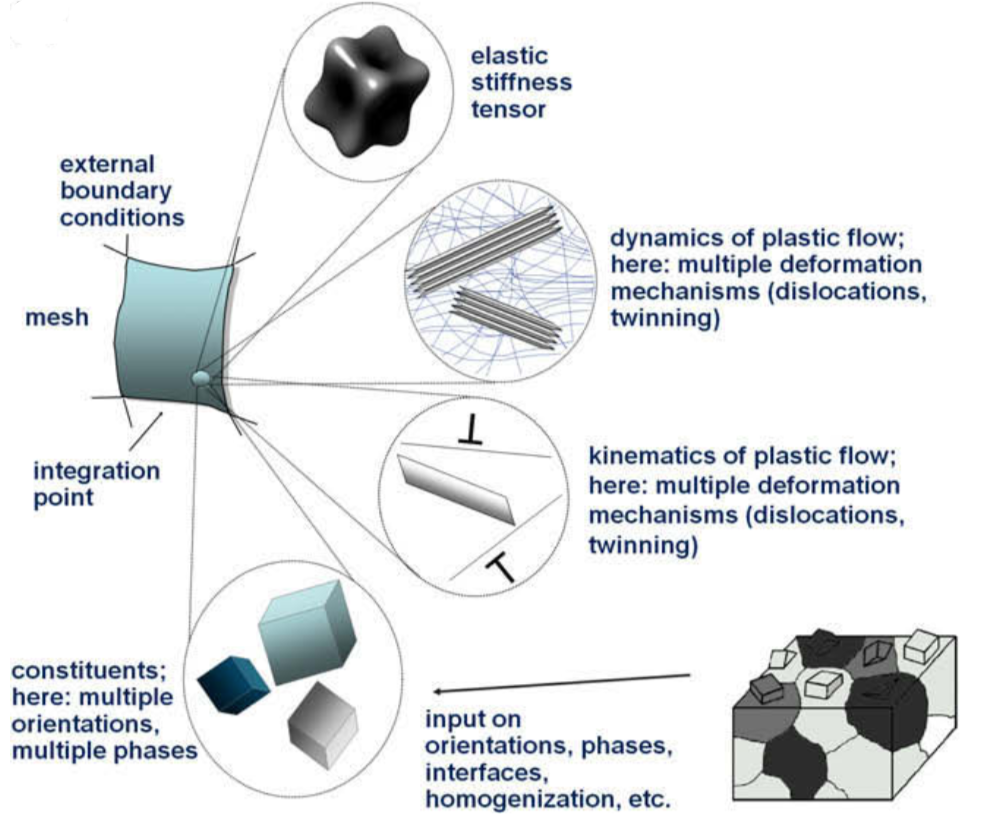
\includegraphics[width=1.0\textwidth]{cpfe.png}
	\hspace{1mm}
	\caption{Schematic representation of CPFE simulations \cite{ROTERS20101152}}  
	\label{fig:cpfe}
\end{figure}

The spatially resolved deformation simulations mentioned above provide high resolution information of the local deformation characteristics and have become the tool of choice for studying the effect of microstructure on the deformation behavior. These predictions are also compared with relevant experimental measurements, where available \cite{POKHAREL2019201} \cite{THOOL2020102785} \cite{Radhakrishnan_2000}. However, these methods generally have large associated computational costs, which may act as a deterrent for performing large number of simulations for advanced computational materials design and screening. In such scenarios, Machine Learning (ML) can be used to develop surrogate models and reduce the computational costs associated with these finite element models \cite{pandey2020machine} \cite{muhammad2020machine} \cite{shen2019convolutional} \cite{MANGAL2018122}.

Machine learning is an emerging research field and has been widely adopted in recent years due to it's outstanding ability to predict properties, relationships and inferences from different kinds of data, with relatively lower computational costs. In the past decade, a variety of surrogate models have been developed and implemented to predict the deformation characteristics of metallic systems. Mangal and Holm \cite{MANGAL2018122} used machine learning to predict the formation of stress hotspots in face centered cubic materials. They implemented a random forest algorithm, which is used for modeling classification and regression problems, in this case classifying grains as stress hotspots, where localized deformation may occur. The algorithm also successfully captured the effect of changing material and texture parameters on the stress hotspots. The model predicted stress hotspots with an accuracy of ~74\%, assuming FFT-based CP simulations as the ground truth. Muhammad et al. \cite{muhammad2020machine} implemented an Artificial Neural Network (ANN) model to predict the local strain distribution, fracture and evolution of plastic anisotropy in additvely manufactured alloys. They were able to predict the location, intensity and the shape of shear bands before failure with high accuracy. The implementation of Convolutional Neural Network (CNN) model has been successfully demonstrated by Beniwal et al. \cite{beniwal2019deep} for predictive modeling of structure-property linkages. This is a reduced order model which has the power to make predictions from just the microstructure image. Deep Learning (DL) based methods have been used to model reverse engineering problems such as using diffraction patterns to reconstruct microstructures \cite{shen2019convolutional}. Kotkunde et al. \cite{kotkunde2014prediction} demonstrated an ANN model to predict the forming limit diagram for sheet metals. A number of parameters such as tool and die geometry and working conditions dictate the sheet metal forming process. The ANN-based approach predicts the forming limit diagram at various combinations of process parameters, otherwise predicted with the help of FE simulations. 

\begin{figure}[!h]
	\centering
	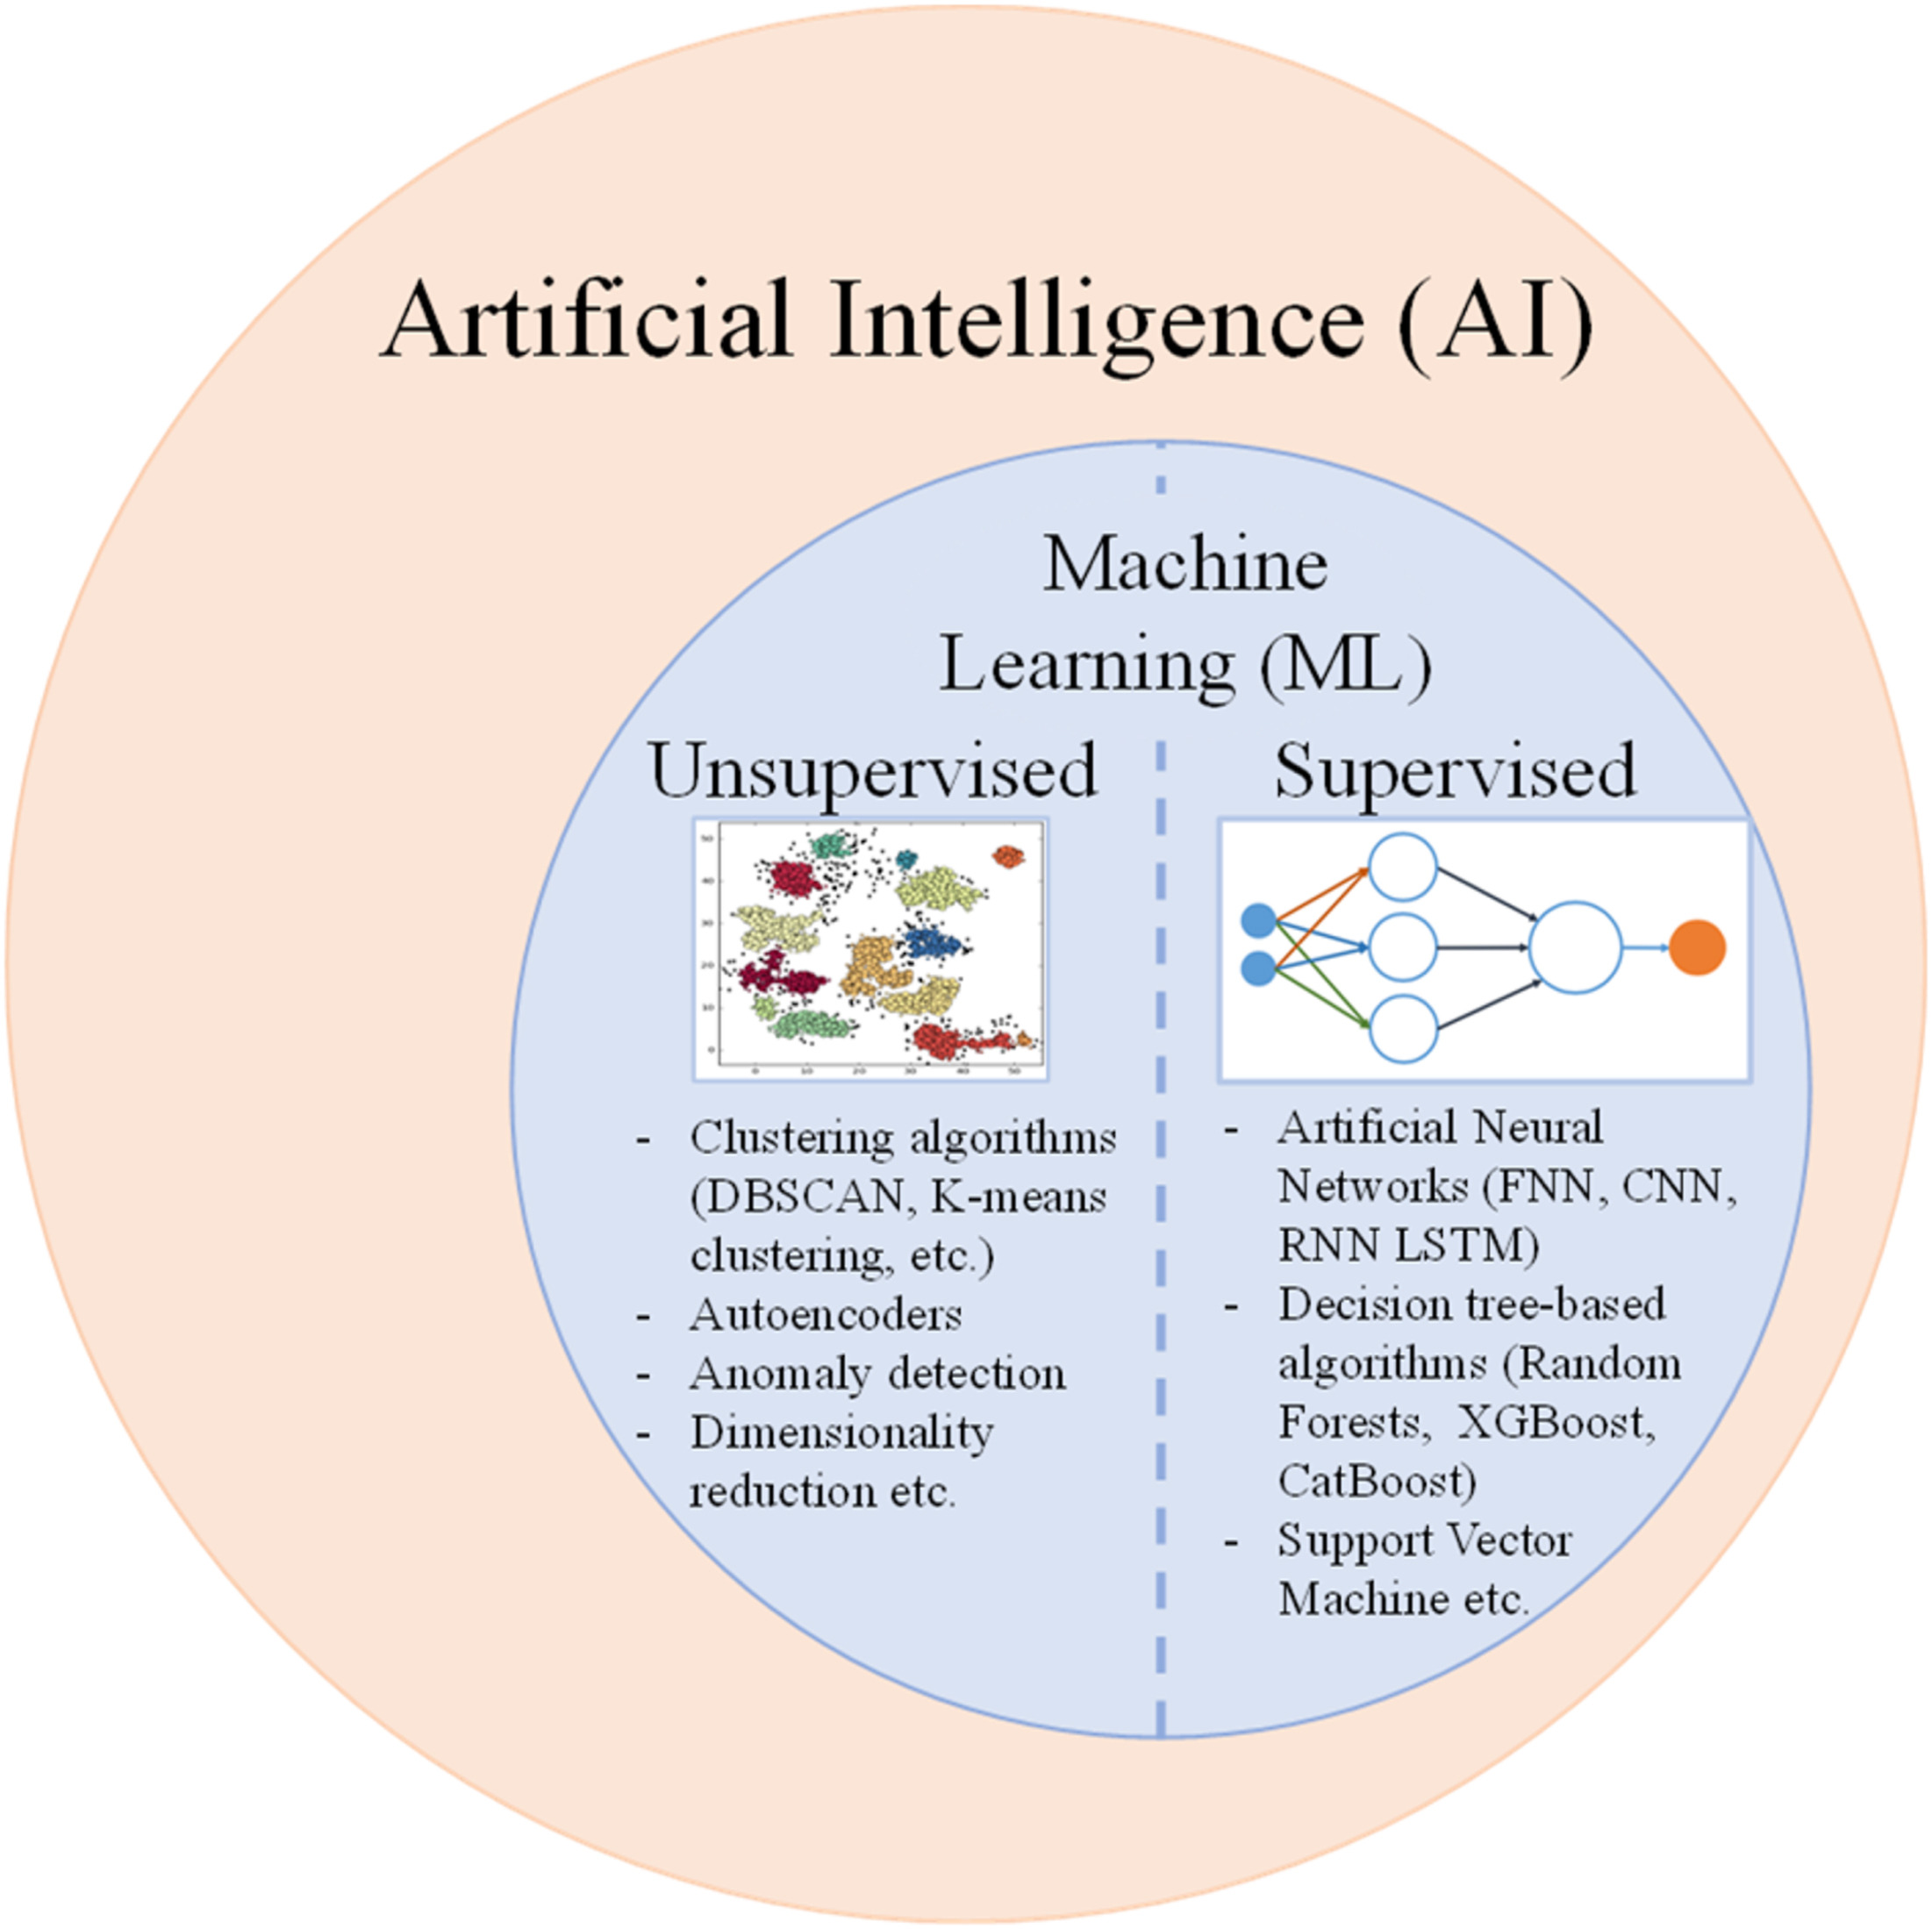
\includegraphics[width=0.7\textwidth]{ml-types.jpg}
	\hspace{1mm}
	\caption{Various types of machine learning models \cite{muhammad2020machine}.} 
	\label{fig:ml-types}
\end{figure}

Further, recurrent Neural Networks (RNN) have been widely for sequence modeling in various fields, but they have shown to be computationally expensive. Recently, a long-short term memory (LSTM) RNN network was proposed, which has the capability of remembering states over time and thus capable of modeling dynamic systems \cite{hochreiter1997long}. Pandey and Pokharel \cite{pandey2020machine} demonstrate a LSTM-based framework for predicting the microstructure evolution under tensile loading of polycrystalline materials. They used a first-order approximation by taking the effect of only nearest neighbor interactions on each crystalline point. Their model doesn't account for any long range interactions and yet produces results with 99\% accuracy. 

Figure \ref{fig:ml-types} shows the classification of some machine learning algorithms commonly used in materials science.

\section{Plan Of Thesis}
A systematic study of various deep learning techniques for predicting the evolution of the deformed microstructure a dual phase (DP) steel has been performed in this thesis. A dislocation density based J2 plasticity finite element framework is used to run deformation simulations of the two phase microstructures of dual phase steels. The J2 plasticity simulations are considered as the ground truth for developing the machine learning model. We start with an ANN and optimize the hyper parameters to achieve the best possible results. Further, as plastic deformation is a history-dependent process, LSTMs are better suited for modeling them as they have the capability to remember states over time. Hence, in the next approaches we show a vanilla LSTM and develop on it to improve our results. The data we are dealing with is spatio-temporal in nature. We demonstrate the ability of LSTM to deal with this kind of data and produce accurate results. 

The subject matter of the thesis is presented in the following 5 chapters:
\begin{itemize}
\item Chapter 2 discusses the fundamentals of deep learning, including the underlying theory of the algorithms used in our work. Further, we discuss some of the approaches used in the literature and their shortcomings.
\item Chapter 3 first provides a summary of the J2 plasticity model used for DP steels. We then discuss the ML model development and implementation.
\item Chapter 4 discusses preliminary results obtained from our model.
\item Chapter 5 summarizes the work done so far and provides details of work planned in the next phase.  
\end{itemize}
\chapter{Review Of Literature} % Main chapter title

\label{Chapter2} % Change X to a consecutive number; for referencing this chapter elsewhere, use \ref{ChapterX}

\lhead{Chapter 2. \emph{Background}}
\label{sec:2}
\section{Introduction To Machine Learning}
Machine Learning (ML) is the sub-field of the much broader concept of Artificial Intelligence. The primary goal of ML, applied to the problem of interest here, is to understand and develop correlations within a given data, which improve automatically through experience. Specifically, these correlations (or mathematical models) are not prescribed \textit{a priori} and are developed by the ML algorithms via analysis of the input data. In classical computing, most algorithms are sets of programmed instructions which the computers use to calculate or solve the problem. ML algorithms on the other hand enable a computer to train on input data and output values that lie within an acceptable range using statistical analysis. Machine learning finds extensive use in many present day technologies. Some real world applications are shown in Figure \ref{fig:app-ml}. 

\begin{figure}[!h]
	\centering
	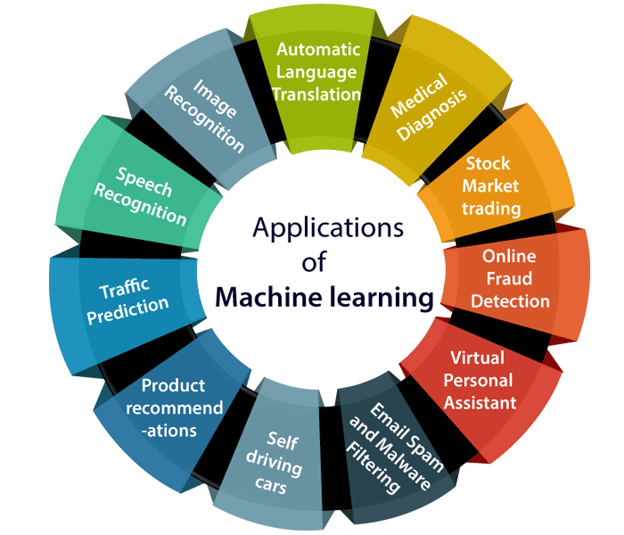
\includegraphics[width=0.7\textwidth]{applications-of-machine-learning.png}
	\hspace{1mm}
	\caption{Various applications of machine learning \cite{mlimage}.} 
	\label{fig:app-ml}
\end{figure}

Deep Learning is a branch of machine learning which is completely based on artificial neural networks. An artificial neural network (ANN) is a flexible mathematical structure which is capable of identifying complex nonlinear relationships between input and output data sets.  It achieves great flexibility and power by learning to represent the world as a nested hierarchy of concepts, with each concept defined in relation to simpler concepts, and more abstract representation computed in terms of less abstract ones \cite{dlintro}. A number of deep learning architectures such as deep neural networks, deep belief networks, recurrent neural networks and convolutional neural networks have been applied to fields including computer vision, speech recognition, natural language processing and audio recognition. These networks have produced results comparable to and in some cases surpassing human expertise. In this thesis, we have employed deep neural networks and recurrent neural networks to develop a model for predicting the deformation behavior.

\section{Deep Learning}
In this section, we describe the fundamentals of neural networks.

\subsection{The Neuron}
A neuron is a fundamental unit of the human brain. The core functionality of a neuron is to input information from other neurons, process it and pass on the results to other cells. It receives information from different connections, which are dynamically strengthened or weakened based on how often it is used (learning new concepts) and this strength determines the effect of the input on the output. Once the inputs are weighted by the strength of their connections, they are summed and transferred to the next neuron. This concept of a neuron can be easily represented on a computer. An artificial neuron has the capability to take in inputs, $x_i, i \in 1,N$ (for $N$ neurons), which are multiplied by their respective weights, $w_i$, and then summed to produce the output or logit of that neuron which can be given as: 
\begin{equation}
z = \sum_{i=1}^{i=n} w_ix_i
\end{equation}

A constant may be added to this logit and then passed through a function $f$ to produce the output $y = f(z)$. The function, $f$, is called the activation function and introduces non-linear behavior in the neuron. Alternatively, the logic may be expressed as a dot product between two vectors, $\boldsymbol{x} = [x_1, x_2,...,x_n]$ as the input vector and $\boldsymbol{w} = [w_1, w_2,...,w_n]$ \cite{buduma2017fundamentals}. The expression thus becomes:
\begin{equation}
y = f(\boldsymbol{w}\cdot\boldsymbol{x} + b)
\end{equation}

\begin{figure}[!h]
	\centering
	
\includegraphics[width=1.0\textwidth]{Pictures/hdnnfin.png}
	\hspace{1mm}
	\caption{Schematic of a neuron.} 
	\label{fig:neuron}
\end{figure}

\subsection{Artificial Neural Network}
A single neuron may not be sufficient to solve or model complicated problems. Analogous to our brain, which is made up of millions of neurons arranged in multiple layers, we can construct an artificial neural network. A neural network consists of a number of neuron hooked to each other. The first layer of nodes receives the input data (input layer) and the last layer's output  (output layer) is the final answer computed by the neural network.  All the layers in between are called the hidden layers. The weight of the connection between the $i^{th}$ neuron in the $k^{th}$ layer with $j^{th}$ neuron in the $(k+1)^{th}$ layer is represented by $w_{i,j}^{(k)}$. Our network's ability to solve problems, is dependent upon finding an optimal value of these weights \cite{buduma2017fundamentals}. Some important aspects of neural networks are as follows:

\begin{enumerate}
\item	Neurons in the same layer have no connections between them and no data is transmitted from a higher layer to a lower layer.
\item	It is not necessary for all the layers to have the same number of neurons.
\item	All the neurons may not have their outputs connected to all the neurons in the next layer. Some connections are dropped to optimize the network and the training process.
\item The input and outputs are vectorized representations.
\end{enumerate}

\begin{figure}[!h]
	\centering
	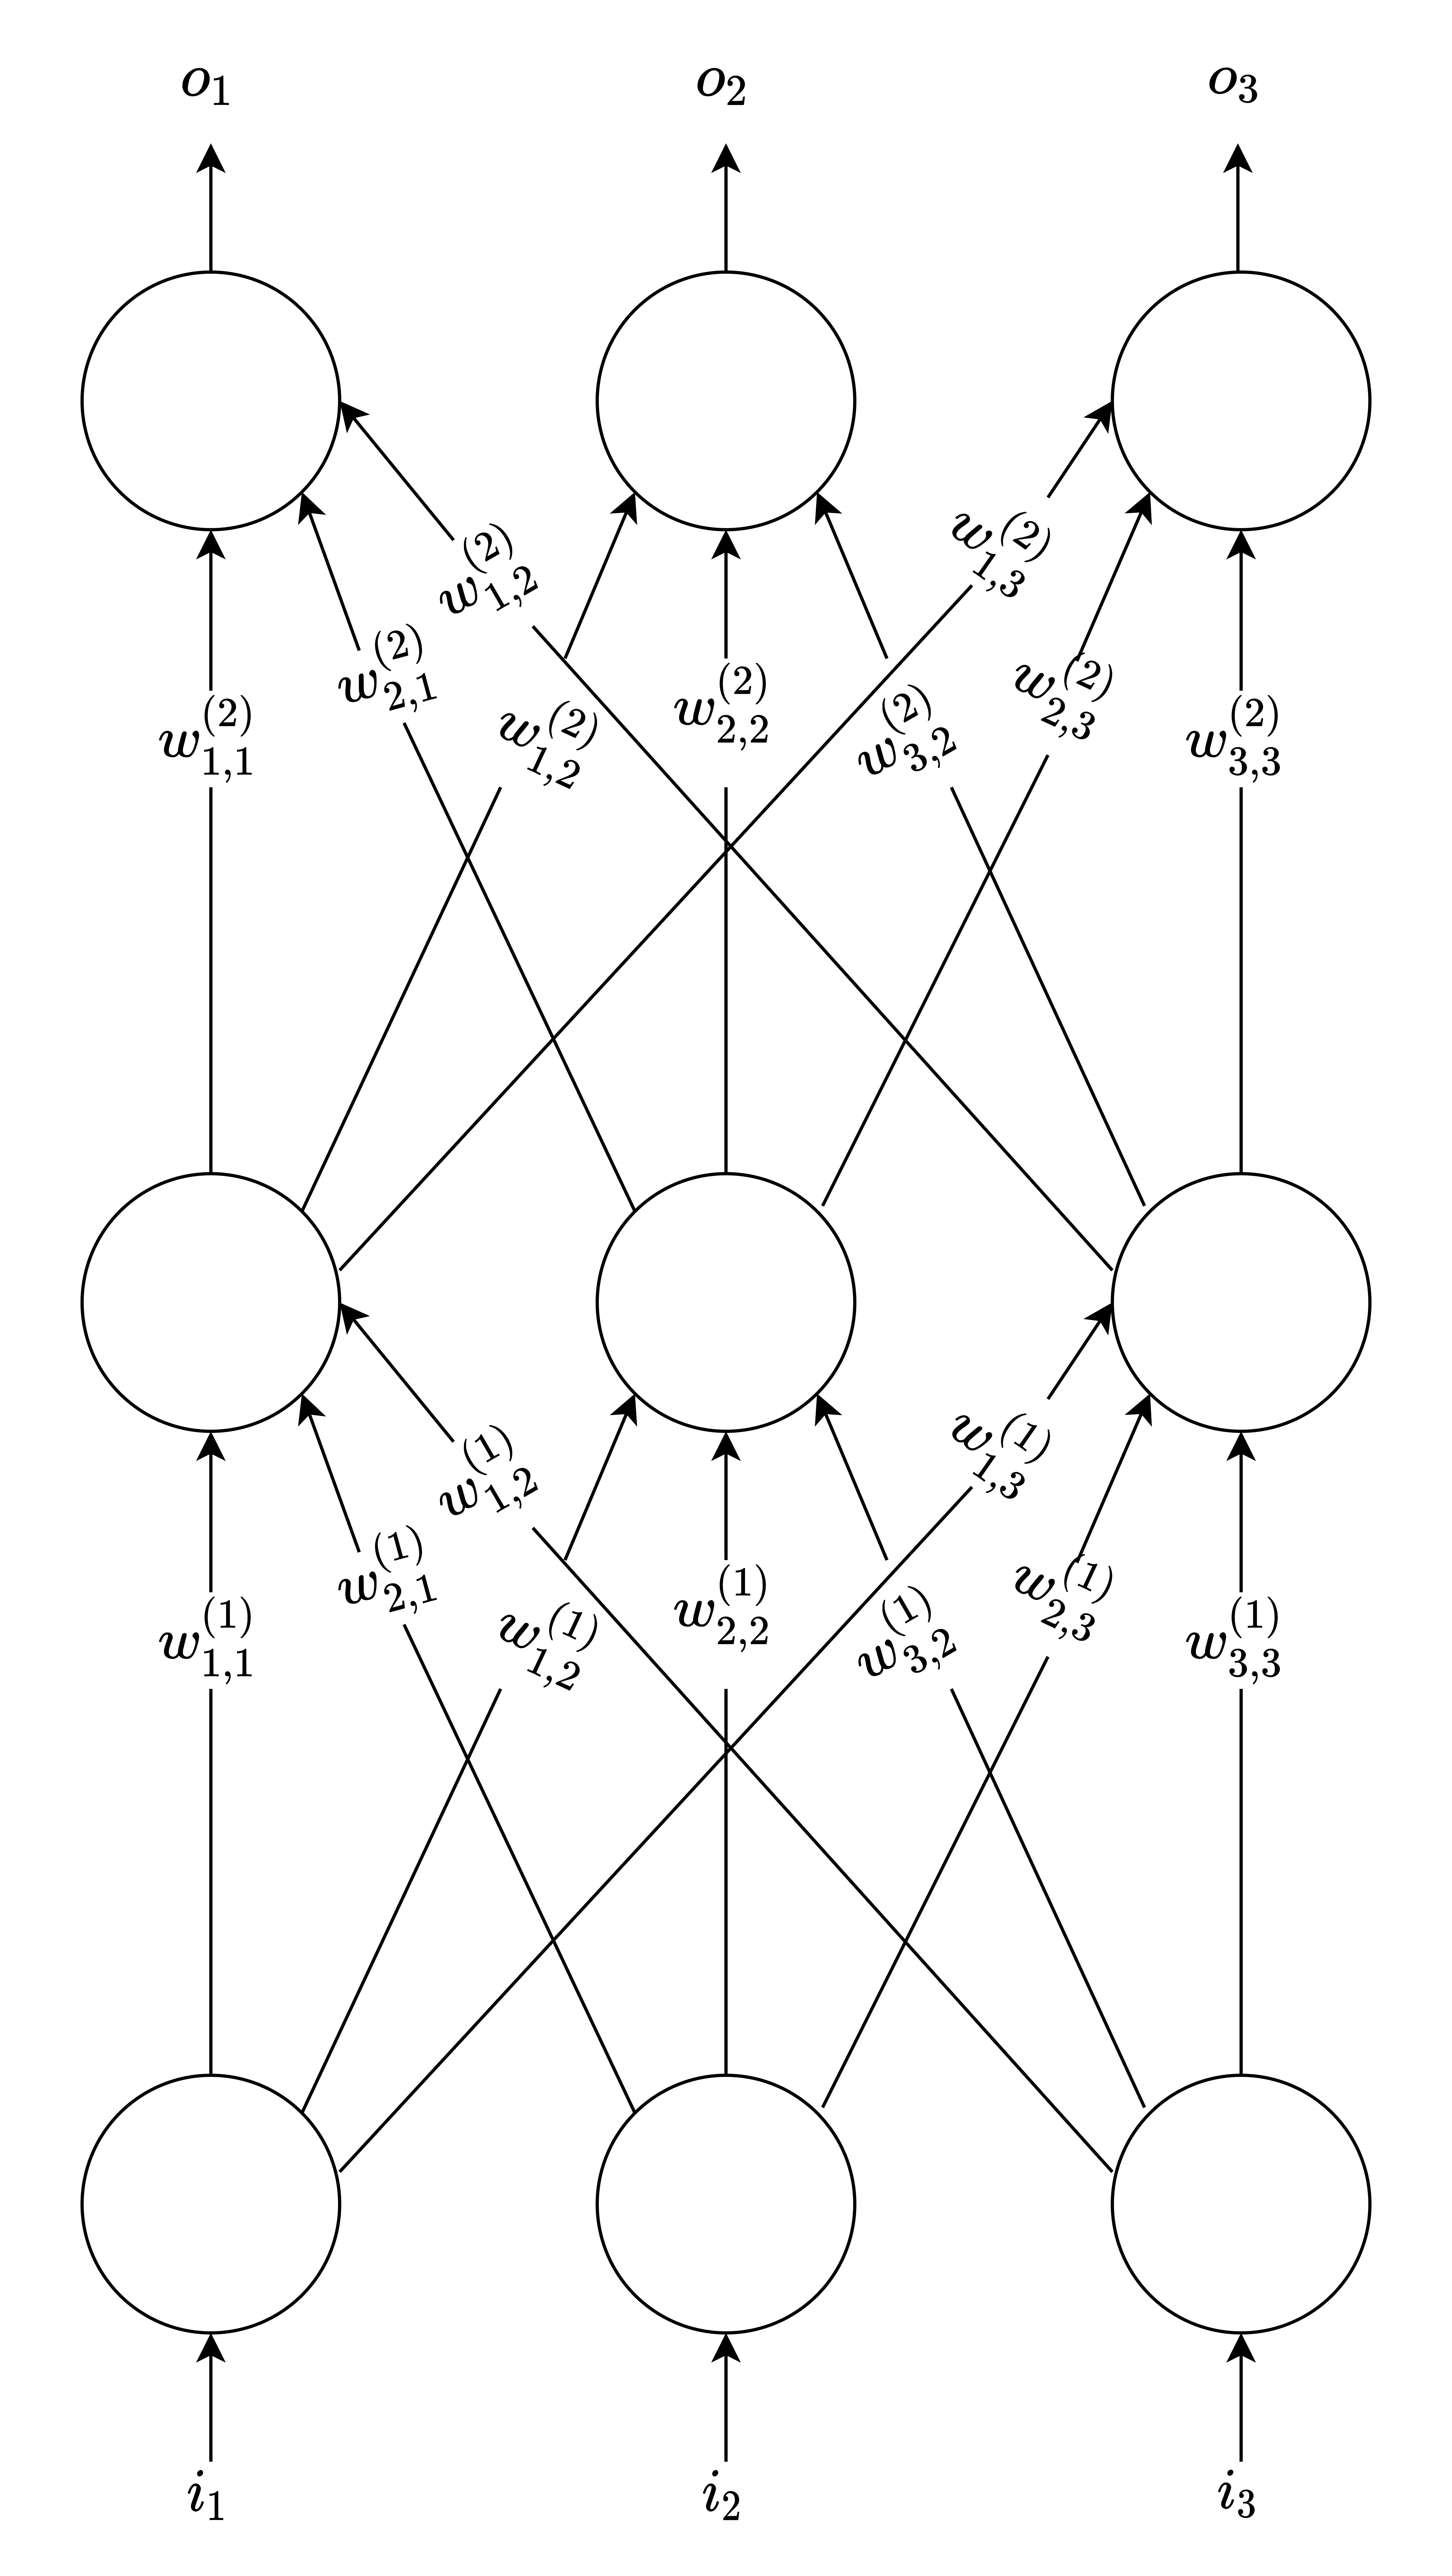
\includegraphics[width=0.45\textwidth]{Pictures/hdaannnpng.png}
	\hspace{1mm}
	\caption{Schematic of a simple neural network.} 
	\label{fig:nn}
\end{figure}

Figure \ref{fig:nn} shows a simple neural network with 3 layers (input layer, 1 hidden layer and output layer) and 3 neurons in each layer. Mathematically, neural networks can be represented as a series of vector and matrix multiplications. Let us say $\boldsymbol{x} = [x_1, x_2,...,x_n]$ is the input to the $i^{th}$ layer, which propagates the output $\boldsymbol{y} = [y_1, y_2,...,y_m]$. We can represent the weights of connections in the form of a weight matrix $\boldsymbol{W}$ of size $m\times n$ along with a bias vector $\boldsymbol{b}$. Then the following holds true:

\begin{equation}
\boldsymbol{y} = f(\boldsymbol{W}^T\boldsymbol{x} + \boldsymbol{b})
\end{equation}

A single neural network can consist of different neurons stacked together in different layers. The activation function, $f$, a neuron applied to their logit, $z$, decides the type of neuron it is. For example, a linear neuron may be of the form: $f(z) = az + b$. A linear neuron is easily computed, but runs into a number of limitations. A network with only linear neurons can mathematically be expressed as a network without hidden layers \cite{buduma2017fundamentals}. Therefore, in order to learn complex relationships we need an activation function which can employ some non-linearity. To help achieve this, there exist 3 major types of neurons. The first one is the sigmoid neuron:

\begin{equation}
f(z) = \frac{1}{1+e^{-z}}
\end{equation}

From the equation above, we can see that for very small logit values the output of the function is close to 0. While for large values of the logit, the output is close to 1. Between 0 and 1, the outputs are as shown in the Figure \ref{fig:sigmoid}.

\begin{figure}[!h]
	\centering
	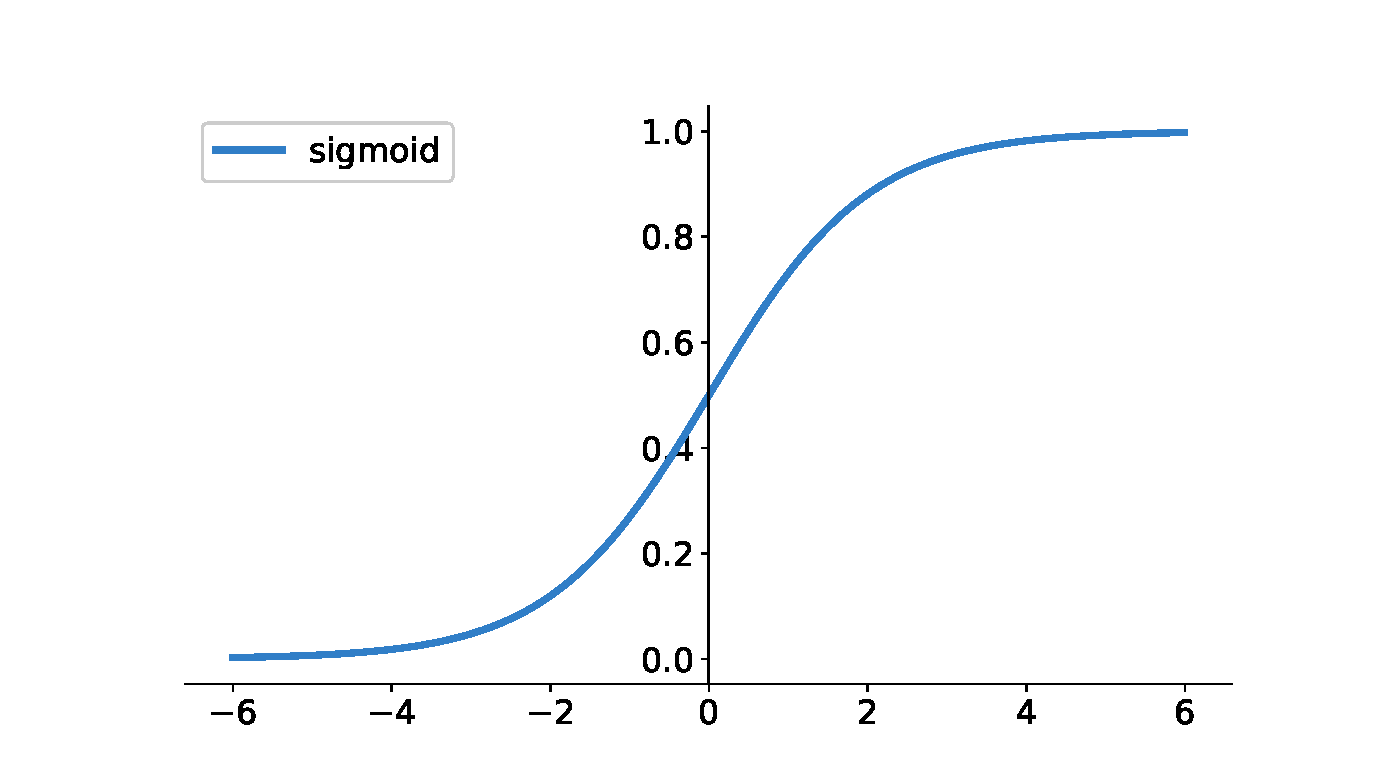
\includegraphics[width=0.7\textwidth]{sigmoid-big.eps}
	\hspace{1mm}
	\caption{Output of sigmoid neuron as a function of z.} 
	\label{fig:sigmoid}
\end{figure}

Another kind of neuron is the tanh neuron, which also uses a similar S-shaped curve but with values ranging from -1 to 1. This is unlike the sigmoid function where values are between 0 and 1. The function is, as expected, $f(z) = tanh(z)$. The relationship between the input logits and output values can be seen in Figure \ref{fig:tanh}.

\begin{figure}[!h]
	\centering
	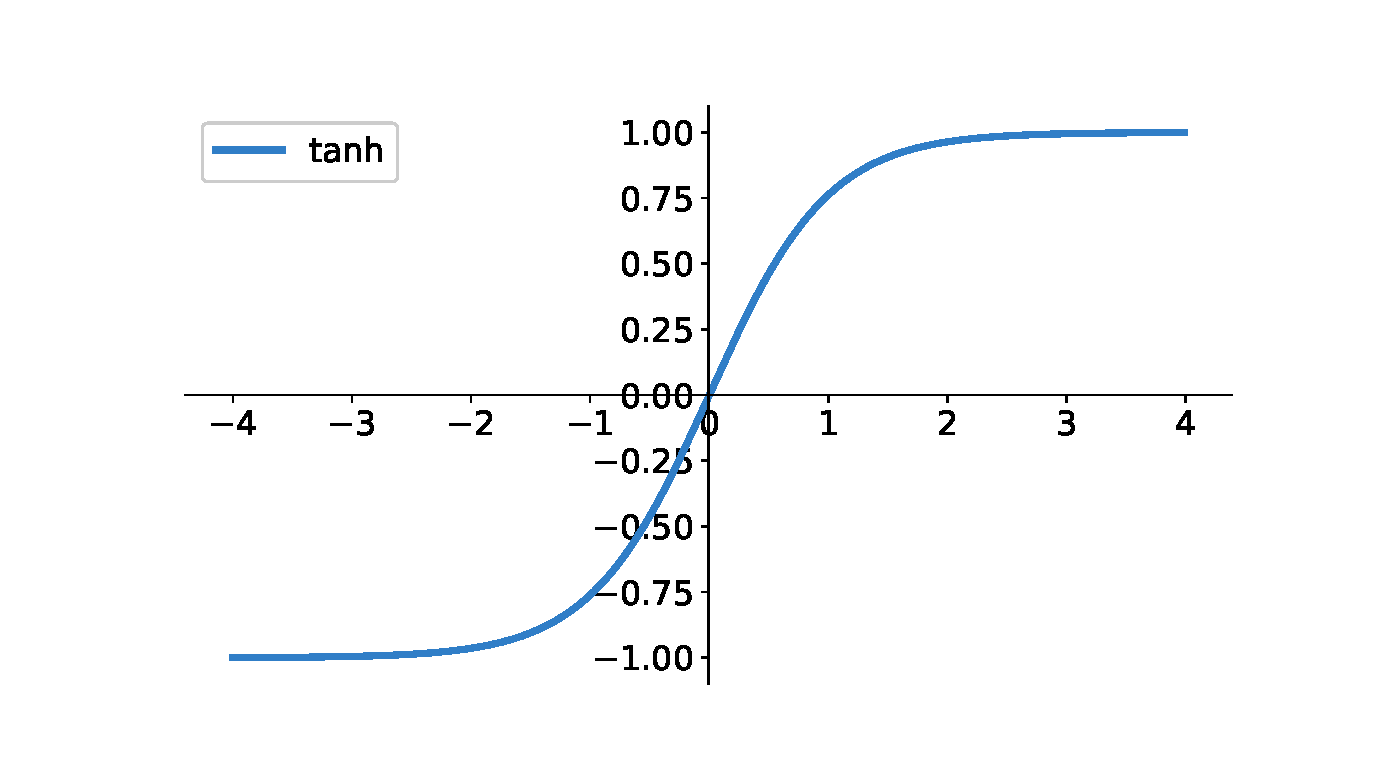
\includegraphics[width=0.7\textwidth]{tanh-big.eps}
	\hspace{1mm}
	\caption{Output of tanh neuron as a function of z.} 
	\label{fig:tanh}
\end{figure}

The last type of neuron we are going to discuss is the restricted linear unit (ReLU) neuron. This function is given by $f(z) = max(0,z)$ resulting in the graph shown in Figure \ref{fig:relu}.

\begin{figure}[!h]
	\centering
	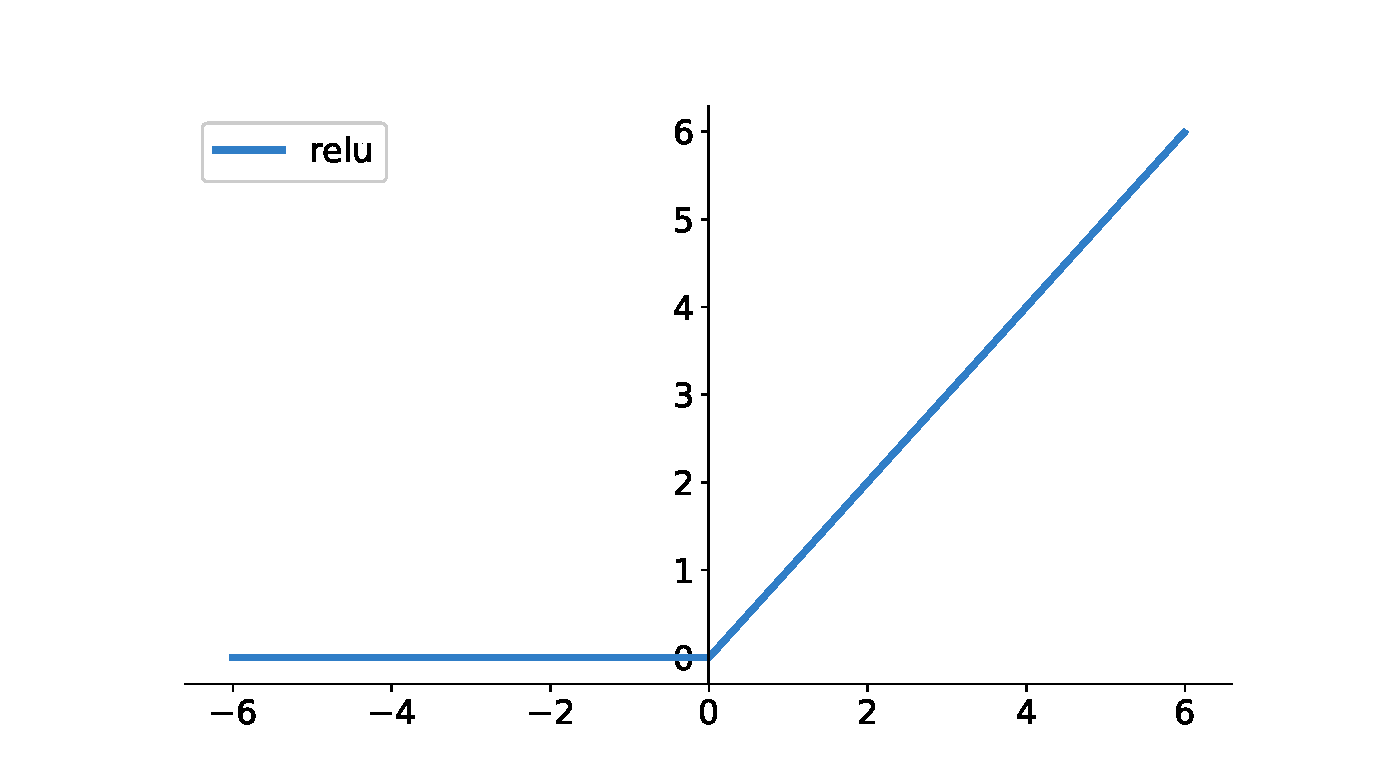
\includegraphics[width=0.7\textwidth]{relu-big.eps}
	\hspace{1mm}
	\caption{Output of ReLU neuron as a function of z.} 
	\label{fig:relu}
\end{figure}

Other activation functions also exist, for example, like exponential linear unit (ELU), binary step, SoftPlus, Leaky ReLU \cite{karlik2011performance}. The ones described in this report are the most commonly used.

\subsection{Training}
A deep learning neural network learns to map a set of inputs to outputs from training data. As there are a large number of unknowns, we cannot calculate the perfect set of weights for the network. Instead, training a neural network is treated as an optimization problem and an algorithm is used to find a set of weights which make relatively good predictions. Before an optimization algorithm is employed we need a metric to measure how well the weights are doing at every step and updating them accordingly. This metric is our loss function and the goal of the training process is to minimize this loss function. There is no one loss function which can be used for all machine learning problems. Choice of the loss function depends primarily on the type of algorithm we are using and the ease with which the function's derivative can be calculated \cite{whytrain}. 

There are two major types of loss functions: regression losses, and classification losses \cite{losses}. In regression, the model deals with predicting a continuous variable like stress, strain for a particular grain. Classification, on the other hand deals with predicting the output from a set of finite categorical value, example labeling a grain as a hotspot. A detailed description of loss functions are given below:

\begin{enumerate}
\item	\textbf{Mean Square Error (MSE)}: is computed from the average of squared difference between actual observations and predictions. The squaring enables heavy penalization of predictions that are far away from the true value. MSE has favorable mathematical properties  of convexity, symmetry, and differentiability. Minimising MSE often has a closed-form analytical solution, and when they do not, iterative numerical optimization procedures are often easy to formulate, since the gradient is easy to compute \cite{4775883}. If $y_i$ is the true value and $\hat{y_i}$ is the predicted value then it can be calculated as: 
\begin{equation}
MSE = \frac{\sum_{i=1}^{n}\left(y_i - \hat{y_i}\right)^2}{n}
\end{equation}
\item	\textbf{Mean Absolute Error (MAE)}: is computed as the averaged sum of absolute difference between actual observations and predictions. However MAE, has proved to under-fit training date due to it's low variance over data points \cite{wang2020imae}. It is given by:
\begin{equation}
MAE = \frac{\sum_{i=1}^n|y_i - \hat{y_i}|}{n}
\end{equation}
\item \textbf{Cross Entropy Loss}: is commonly used for classifications problems. Cross-entropy loss increases as the predicted probability diverges from the actual label. The mathematical formulation is given as: 
\begin{equation}
Cross Entropy Loss = -(y_ilog(\hat{y_i}) + (1-y_i)log(1-\hat{y_i}))
\end{equation}
\end{enumerate}

Having described the loss functions, we now describe an algorithm to find the weights and biases so that the network's output approximates well for all training inputs. We start with looking at a simpler version of the mean squared error cost function and later generalize for a neural network. The cost function can be written as follows:
\begin{equation}
C(\boldsymbol{w},\boldsymbol{b}) = \frac{\displaystyle\sum\limits_x ||y(x) - a||^2}{n}
\end{equation}
Here, $\boldsymbol{w}$ and $\boldsymbol{b}$ denote the weights and biases respectively, $n$ is the number of training inputs and $a$ is the output from the network. The aim of the optimization algorithm is to minimise this cost function: the training algorithm has done well if it can find weights and biases such that $C(\boldsymbol{w},\boldsymbol{b})\approx 0$. To achieve this we use a gradient descent algorithm. Currently the problem looks very complicated - the interpretation of $\boldsymbol{w}$ and $\boldsymbol{b}$ and the summation function in the background. Let us ignore most of these structures and just concentrate on the minimization aspect. Let us further assume that we have a function of two variables $w_1$ and $w_2$, and we want to minimise this function. So our new function is $C(w_1, w_2)$, and for small changes $\Delta w_1$, $\Delta w_2$ the corresponding change in $C(w_1, w_2)$ can be given as:
\begin{equation}
\Delta C \approx \frac{\partial C}{\partial w_1}\Delta w_1 + \frac{\partial C}{\partial w_2}\Delta w_2
\end{equation}
We can define vector as $\boldsymbol\Delta w = (\Delta w_1, \Delta w_2)^T$ and the gradient vector by $\boldsymbol\nabla C$. The gradient vector, $\boldsymbol\nabla C$, is the direction of steepest descent for any function, hence we move along this direction.
\begin{equation}
\boldsymbol{\nabla C} = \left(\frac{\partial C}{\partial w_1}, \frac{\partial C}{\partial w_2}\right)^T
\end{equation}
With these definitions, Equation 2.9 can be written as
\begin{equation}
\Delta C \approx \boldsymbol{\nabla C}\cdot \boldsymbol \Delta w
\end{equation}
We want $\Delta C$ to always be negative because we want to minimise the function. We can choose our $\Delta v$ such that $\Delta C$ is always negative. \cite{nielsen2015neural}
\begin{equation}
\boldsymbol\Delta w = -\eta\boldsymbol\nabla C
\end{equation}
$\eta$ is a small positive character known as the learning rate. It is a hyperparameter that controls how much one should adjust the model in response to the estimated error everytime the weights are updated. Very small a value may cause results in a long training process, whereas a large value may always yield a sub-optimal set of weights and never converge \cite{learningrate}. Selection of learning rate is also another crucial step in the training process. Moving on, from Equation 2.11 we can say $\Delta C \approx -\eta\boldsymbol\nabla C\cdot \boldsymbol\nabla C = -\eta||\boldsymbol\nabla C||^2$. As $||\boldsymbol\nabla C||^2 \geq 0$, this guarantees that $\Delta C \leq 0$, i.e., $C$ will always decrease. Thus, the weights can be updated using the following rule:
\begin{equation}
\boldsymbol w \rightarrow \boldsymbol w^{'} = \boldsymbol w - \eta\boldsymbol\nabla C
\end{equation} 

\begin{figure}[!h]
	\centering
	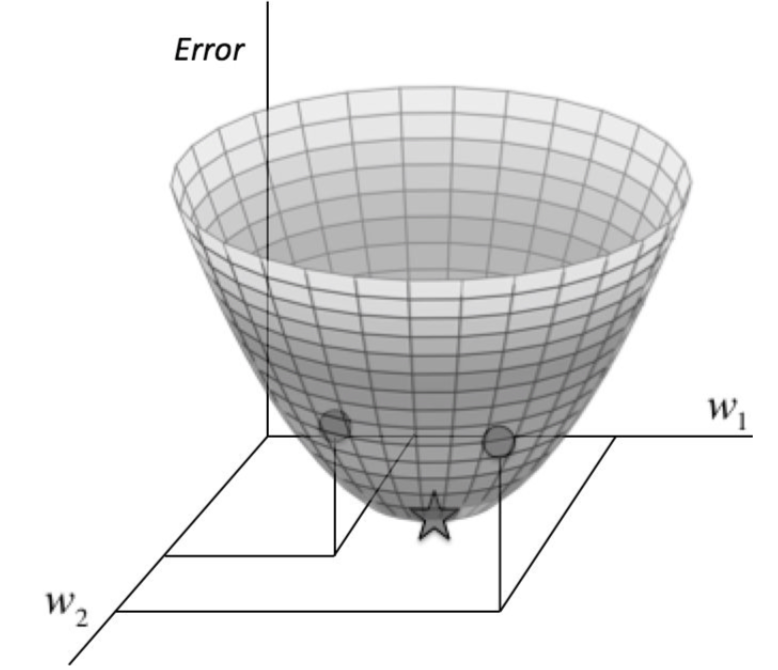
\includegraphics[width=0.6\textwidth]{2-var-grad.png}
	\hspace{1mm}
	\caption{Error surface as a function of $w_1$ and $w_1$} 
	\label{fig:err-surf}
\end{figure}
The above example as we spoke earlier is a very simplified case with just two weights taken into consideration. But actual neural networks have a large number of weights and biases segregates into different layers. We need a systematic algorithm to update all the values according to the error. Back-propagation helps in understanding how changing the weights and biases changes the cost function. Before we get started let us define some notations: $w_{jk}^l$ denotes the weight for the connection from $k^{th}$ neuron in the $(l-1)^{th}$ layer to the $j^{th}$ neuron in the $l^{th}$ layer. Similarly for biases, $b_j^l$ for the bias of $j^{th}$ neuron in the $l^{th}$ layer. $a_j^l$ will be used for the activation. $L$ denotes the last layer in the network. The goal of back-propagation is to compute partial derivatives, $\partial C/\partial w$ and $\partial C/\partial b$, with respect to any weight or bias. Let us say we introduce an error $\Delta z_j^l$ in the logit of the $j^{th}$ neuron in the layer $l$. This will change the output give by this neuron's activation function and propagate through the later layers finally cost function to change by $\frac{\partial C}{\partial z_j^l}\Delta z_j^l$. Thus in some sense we can define the error in that neuron by
\begin{equation}
\delta_j^l = \frac{\partial C}{\partial z_j^l}
\end{equation}
$\boldsymbol{\delta^l}$ will denote the vector of errors assiciated with layer $l$. Using backpropagation we will be able to calculate $\boldsymbol{\delta^l}$ for all the layers and relates those to our variables of interest through, $\partial C/\partial w_{jk}^{l}$ and $\partial C/\partial b_j^l$. The backpropagation algorithm is based on four fundamental equations which give us a way of computing both the gradient of the cost function and error $\boldsymbol{\delta^l}$ \cite{nielsen2015neural}.
\begin{enumerate}
\item \textbf{Error in output layers}: is given below. The $\partial C/\partial a_j^L$ measures how fast the cost function changes with the activation of the $j^{th}$ neuron in the output layer. The second term accounts for changes in the activation function $\sigma$ with changes in $z_j^L$.
\begin{equation}
\delta_j^l = \frac{\partial C}{\partial a_j^L}\sigma^{\prime}(z_j^L)
\end{equation}
The equation can be re-written for all neurons using matrix-based form using  Hadamard product, which is basically the element-wise product of two vectors.
\begin{equation}
\boldsymbol{\delta^L} = \nabla_a C \odot \sigma^{\prime}(z^L)
\end{equation}
\item \textbf{Error in terms of error in the next layer}: is given below where $(w^{l+1})$ is the weight matrix for the $(l+1)^{th}$ layer. If we know the error $\boldsymbol{\delta^{l+1}}$ for $(l+1)^{th}$ layer, then by mutiplying the transpose of the weight matrix we move the error backward through the network to give us the measure of error at the $l^{th}$ layer. By taking the Hadamard product with $\sigma^{\prime}(z^L)$ the error moves backward through the activation layer, giving us $\boldsymbol{\delta^l}$ for that layer.
\begin{equation}
\boldsymbol{\delta^l} = ((w^{l+1})^T \delta^{l+1})\odot \sigma^{\prime}(z^l)
\end{equation}
Using the equations above, we can calcualte the $\boldsymbol{\delta^l}$ for any layer starting with the output layer. 
\item \textbf{Change of error with bias}: is a simple equation given by:
\begin{equation}
\frac{\partial C}{\partial b_j^l} = \delta_j^l
\end{equation}
\item \textbf{Change of cost with any weight}: can now easily be given by the following equation. We already know how to compute $\boldsymbol{a^{l-1}}$ and $\boldsymbol{\delta^l}$.
\begin{equation}
\frac{\partial C}{\partial w_{jk}^l} = a^{l-1}_k \delta^l_j
\end{equation}
\end{enumerate}

\subsection{Recurrent Neural Networks}
Recurrent Neural Networks (RNNs) have played an important role in the field of machine learning ever since their introduction and development in the 1990s. They are used to learn time-varying and sequential patterns. \cite{medsker2001recurrent} RNNs leverage a special type of neural layer, known as recurrent layers which makes different from a neural network. The recurrent layer enables the network to maintain state between the uses of the network. All the neurons in an RNN have three types of connections: (i) incoming connections from the neuron of the previous layer (input) (ii) outgoing connections leading to neurons in the next layer (output), and (iii) recurrent connections between neurons in the same layer. Thus, a fully connected recurrent layer has information flowing from every neuron to every other neuron in the same as well as the next layer (including itself). A recurrent layer with $r$ neurons has $r^2$ connections within the same layer.
\begin{figure}[!h]
	\centering
	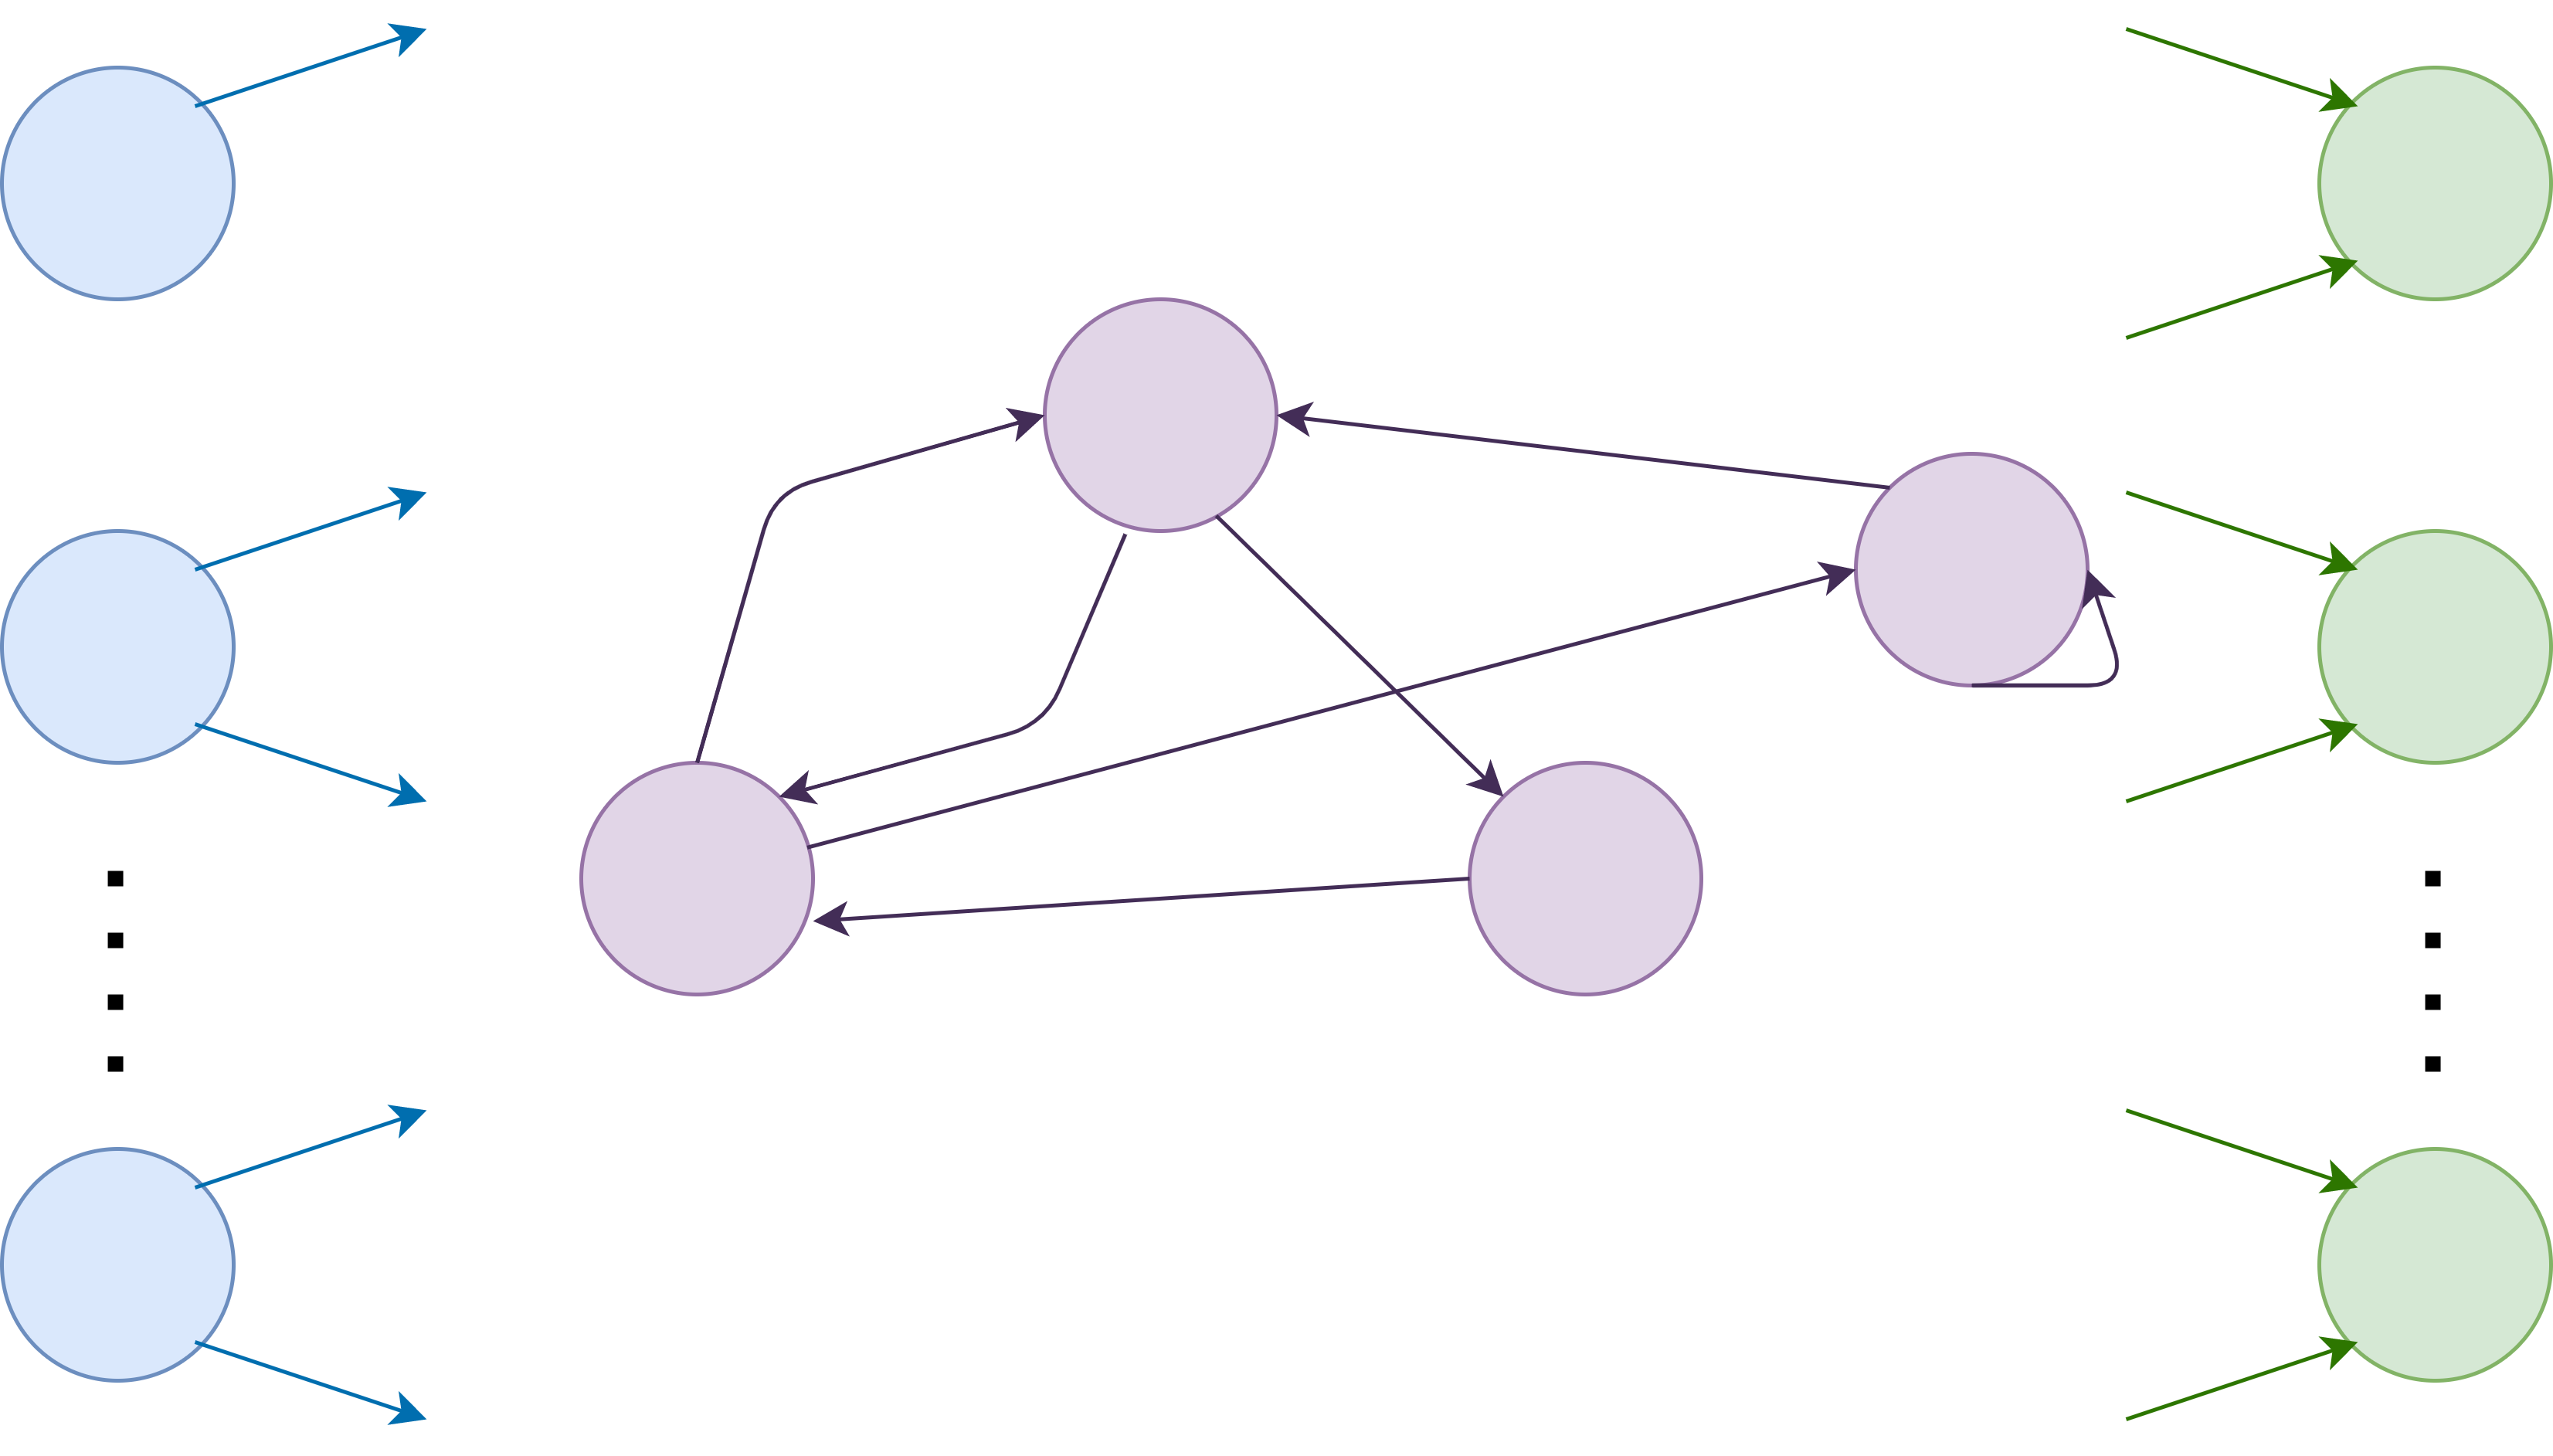
\includegraphics[width=0.6\textwidth]{Pictures/rnn-layer.png}
	\hspace{1mm}
	\caption{A recurrent layer with connections between neurons in the same layer. } 
	\label{fig:err-surf}
\end{figure}

RNNs are a category of neural networks where output from the previous time steps is taken as input for the current time-step. A RNN instance can actually be expressed as a feed forward neural network for a given fixed lifetime ($t$ time-steps). This transformation is referred to as "unrolling" the RNN through time. The update graph formed by unrolling is a useful way to visualise RNNs. The transformation is performed by repeating the neurons in the recurrent layer $t$ times, once for each time-step. Similarily the input and output connections are redrawn as they were in the original network and all the feed forward connections are made. Finally, feed forwards connections are drawn from each time-step replica to the next time-step as recurrent neural networks use neuronal activation from the previous time-step. Consider an input with $T$ timesteps, $I$ input units, $H$ hidden units, and $K$ output units. Let $x_i^t$ be the input $i$ at time $t$, $z_j^t$ be the input logit at of unit $j$ and $y_j^t$ be the activation. Then for hidden units, the logit can be written as
\begin{equation}
z_h^t = \sum_{i=1}^{I} w_{ih}x_i^t + \sum_{h^\prime =1}^H w_{h^\prime h}y_{h^\prime}^{t-1}
\end{equation}
\begin{figure}[!h]
	\centering
	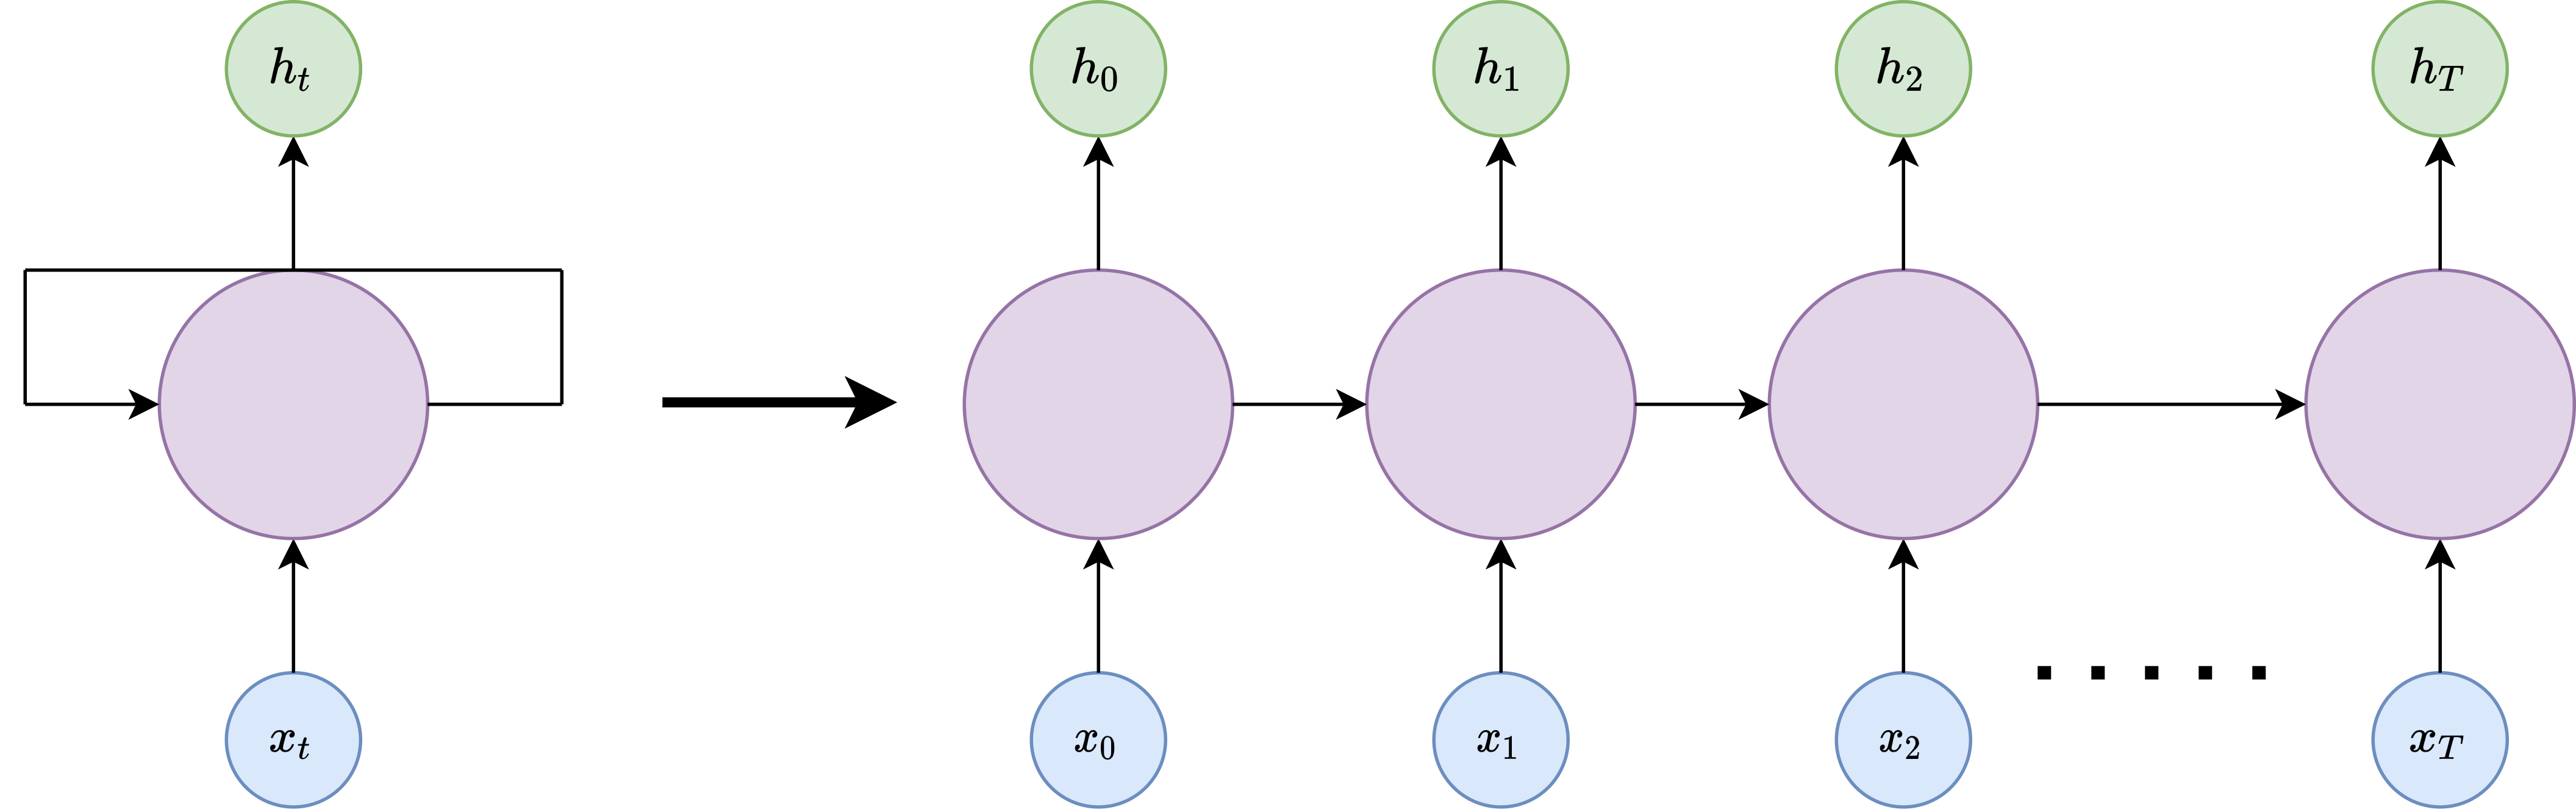
\includegraphics[width=0.85\textwidth]{Pictures/unrolled-rnn.png}
	\hspace{1mm}
	\caption{RNN unrolled over time} 
	\label{fig:err-surf}
\end{figure}

The unrolled RNN can be trained by computing the gradient and using the techniques used for a feed forward neural network. However, for standards RNN architectures the range of context that can be accessed is quite limited. The influence of the inputs on the hidden layers either decays or blows exponentially as it cycles around the network's recurrent connections. This is often referred to as the problem of vanishing gradient \cite{hochreiter1998vanishing}. It is depicted in the figure given below. The shade of the node in the unrolled RNN indicates the relevance of the input at the first time step (darker the shade, greater the sensitivity). Numerous attempts were made to solve this problem, one of which is long short-term memory networks. 
\begin{figure}[!h]
	\centering
	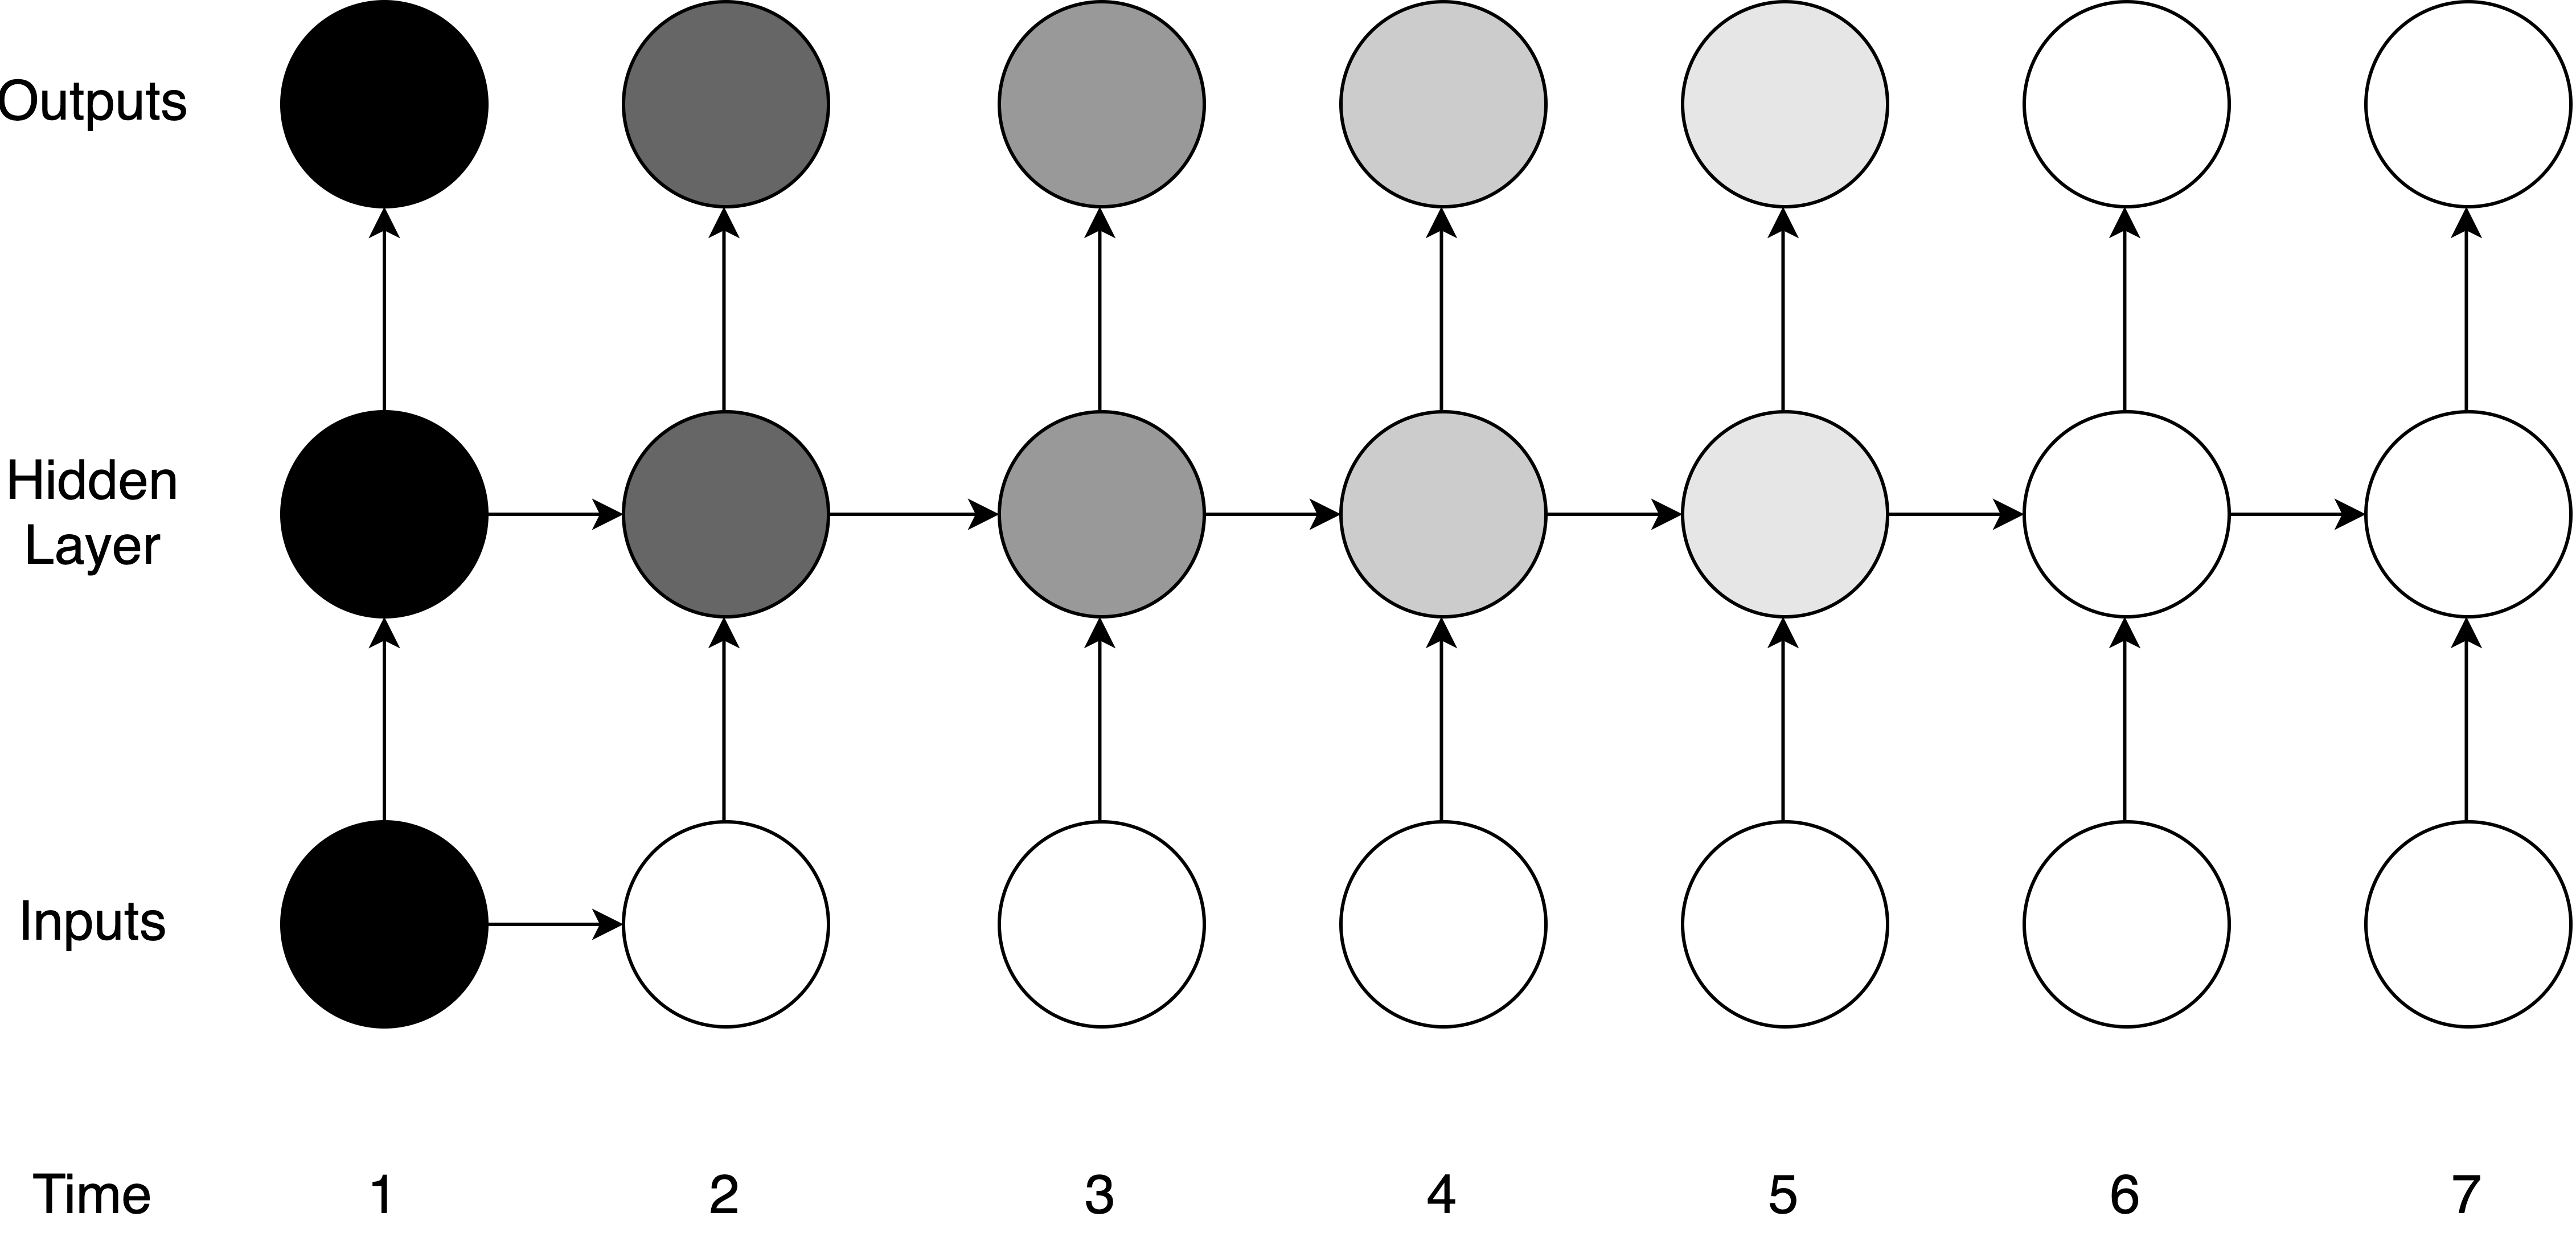
\includegraphics[width=0.85\textwidth]{Pictures/vanishing-grad.png}
	\hspace{1mm}
	\caption{Vanishing gradient.} 
	\label{fig:err-surf}
\end{figure}

\subsection{Long Short-Term Memory (LSTM) Networks}
Long short-term memory networks were introduced by Hochreiter and Schmidhuber with the basic principle that the network would be designed for transmitting useful information multiple time-steps into the future  \cite{hochreiter1997long}. The LSTM architecture consists of memory cells, which are recurrently connected sub-nets. This memory cell is responsible for holding important information that the network has learnt over time and the network is designed to maintain this information with time. The memory cell functions with the help of three gates, which are discussed next. The schematic of a LSTM unit \hat{y_i} can be seen in figure-\ref{fig:lstm-cell}.
\begin{figure}[!h]
	\centering
	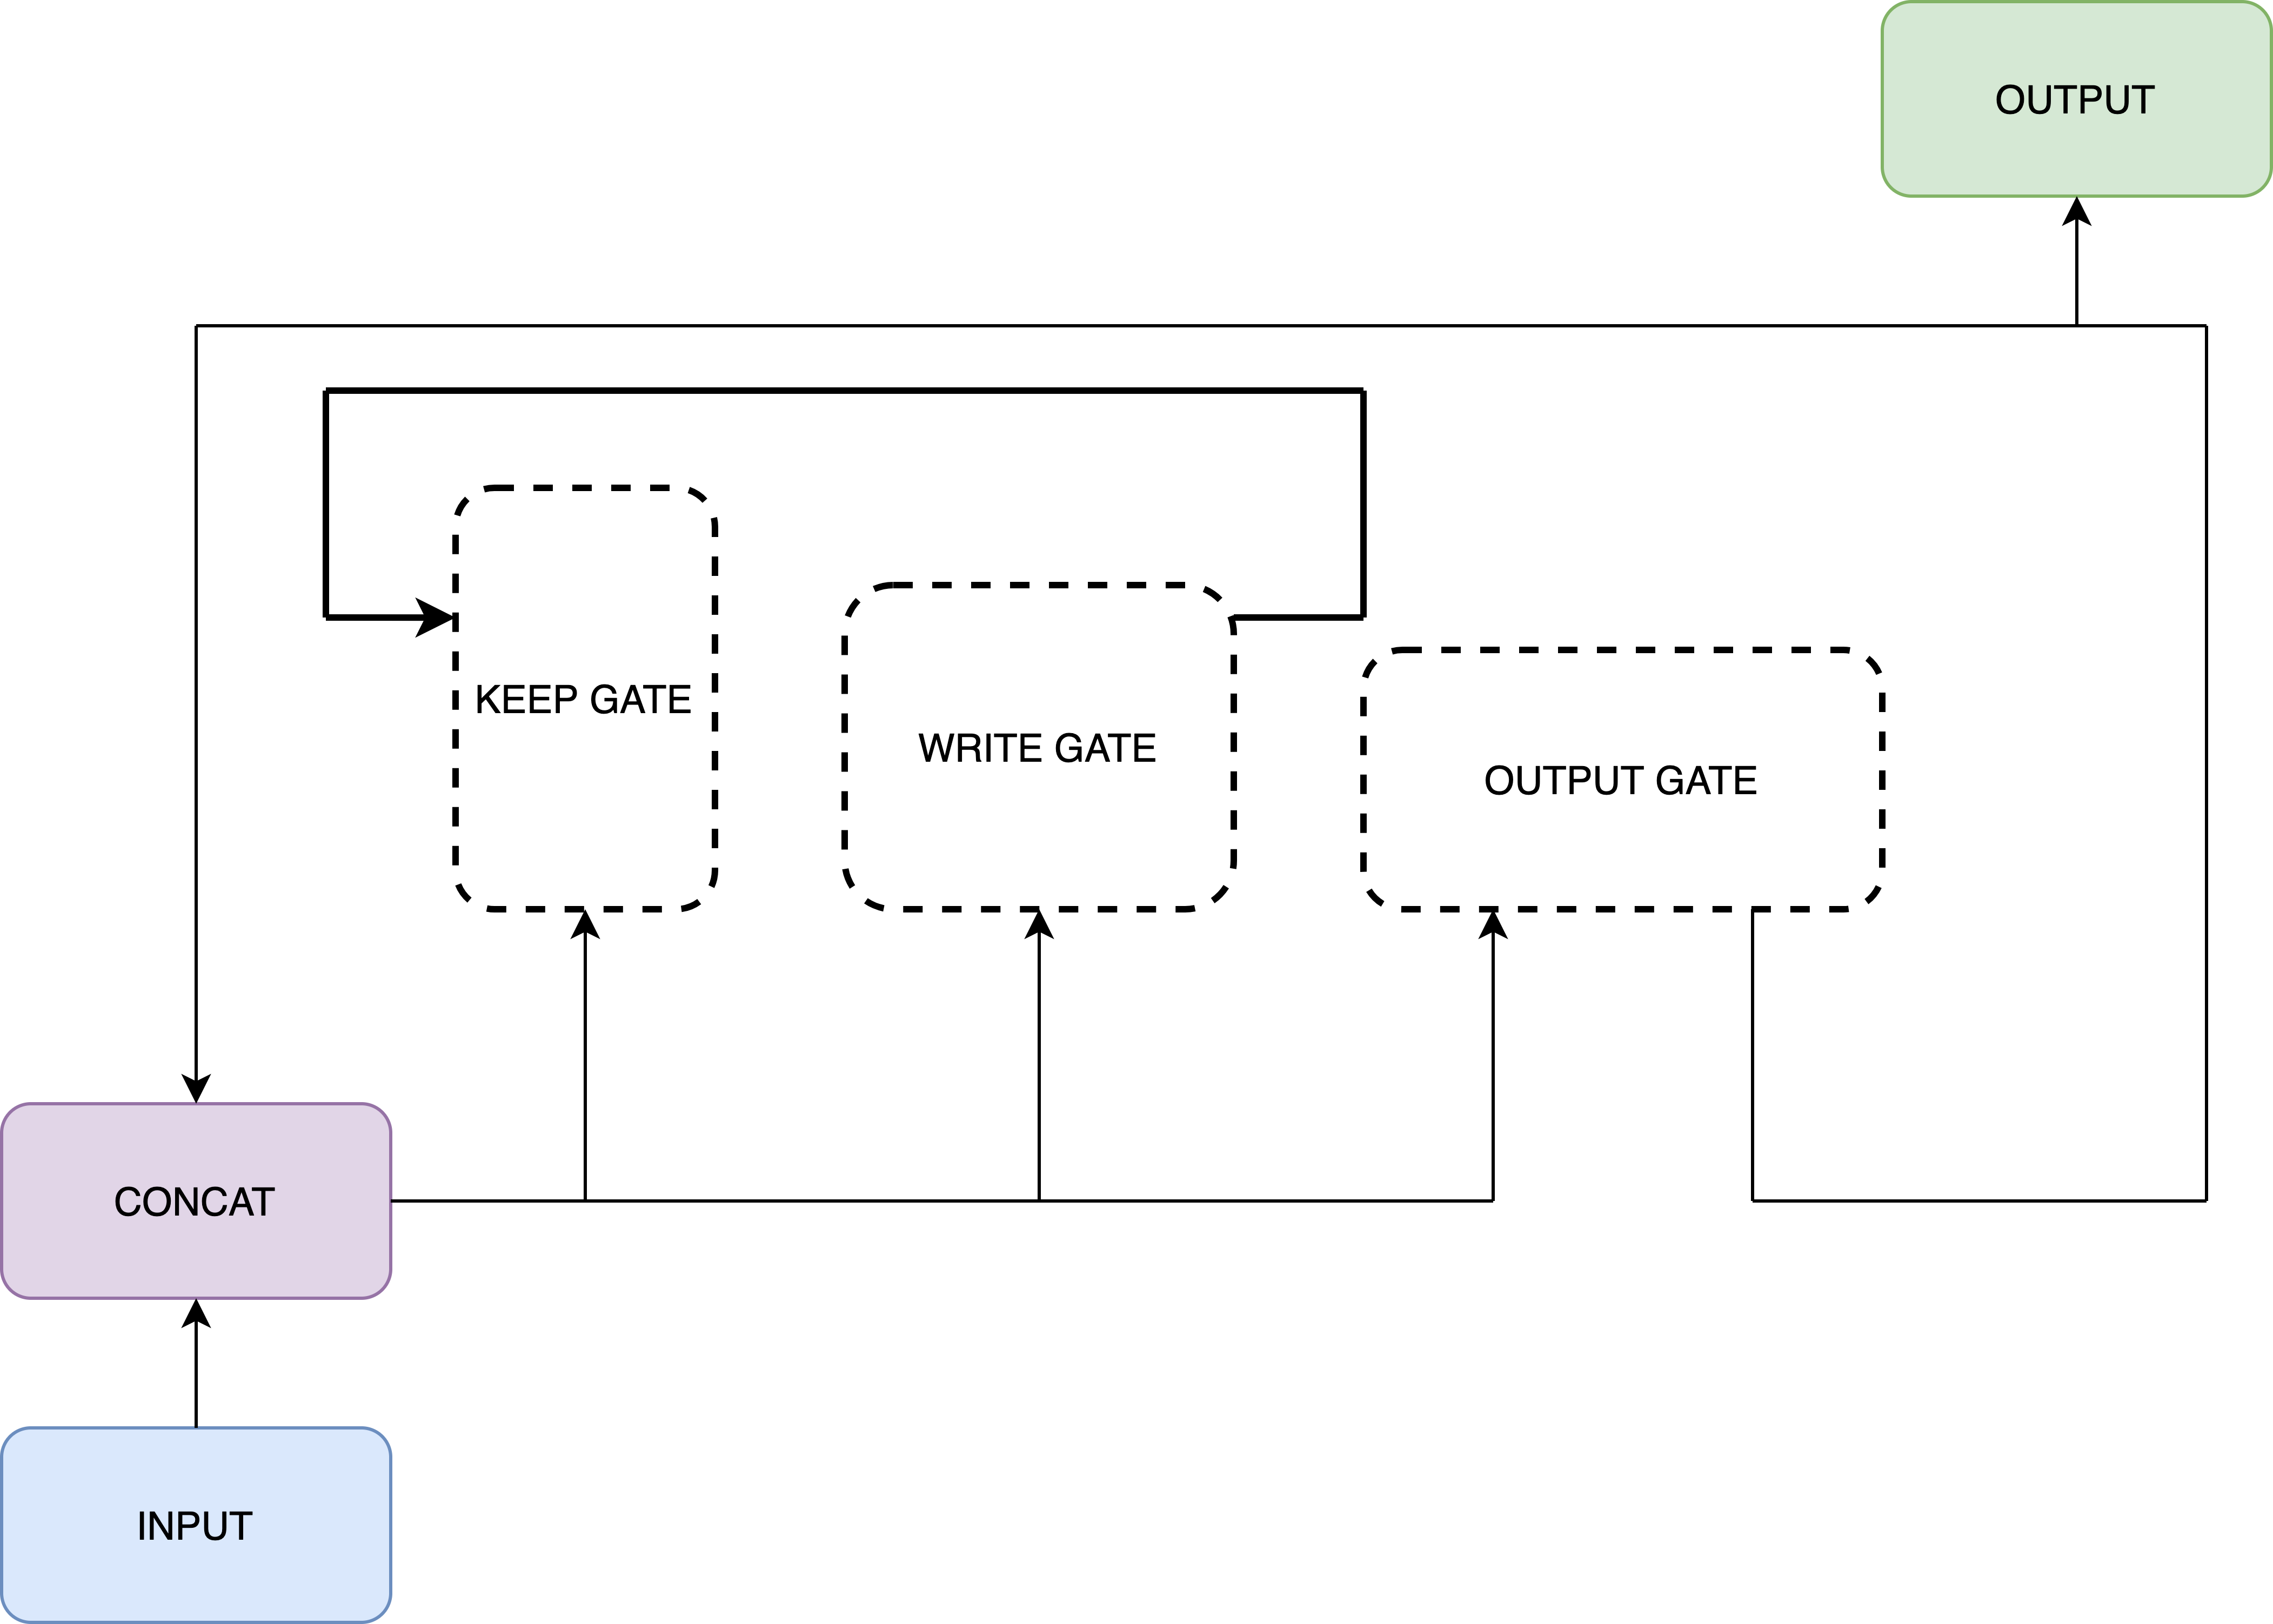
\includegraphics[width=0.85\textwidth]{Pictures/lstm-cell.png}
	\hspace{1mm}
	\caption{A LSTM unit.} 
	\label{fig:lstm-cell}
\end{figure}

The memory cells have a keep gate, shown in figure-\ref{fig:keep-gate}, which determines how much of the previous memory is useful and will be stored for future use. Memory state from the previous time-step is stored in the form of a tensor, rich in information. To figure out the elements in the memory tensor which are still useful, a bit tensor (tensor of zeros and ones) is calculated that we multiply to the memory state tensor. Intuitively, a zero means that the element's information is useless and one means that it is useful. The bit tensor is approximated by concatenating the output from the previous time-step along with the input of this time-step and applying a sigmoidal activation to them. The sigmoid function outputs value very close to 1 or 0 and hence works well for this task. 
\begin{figure}[!h]
	\centering
	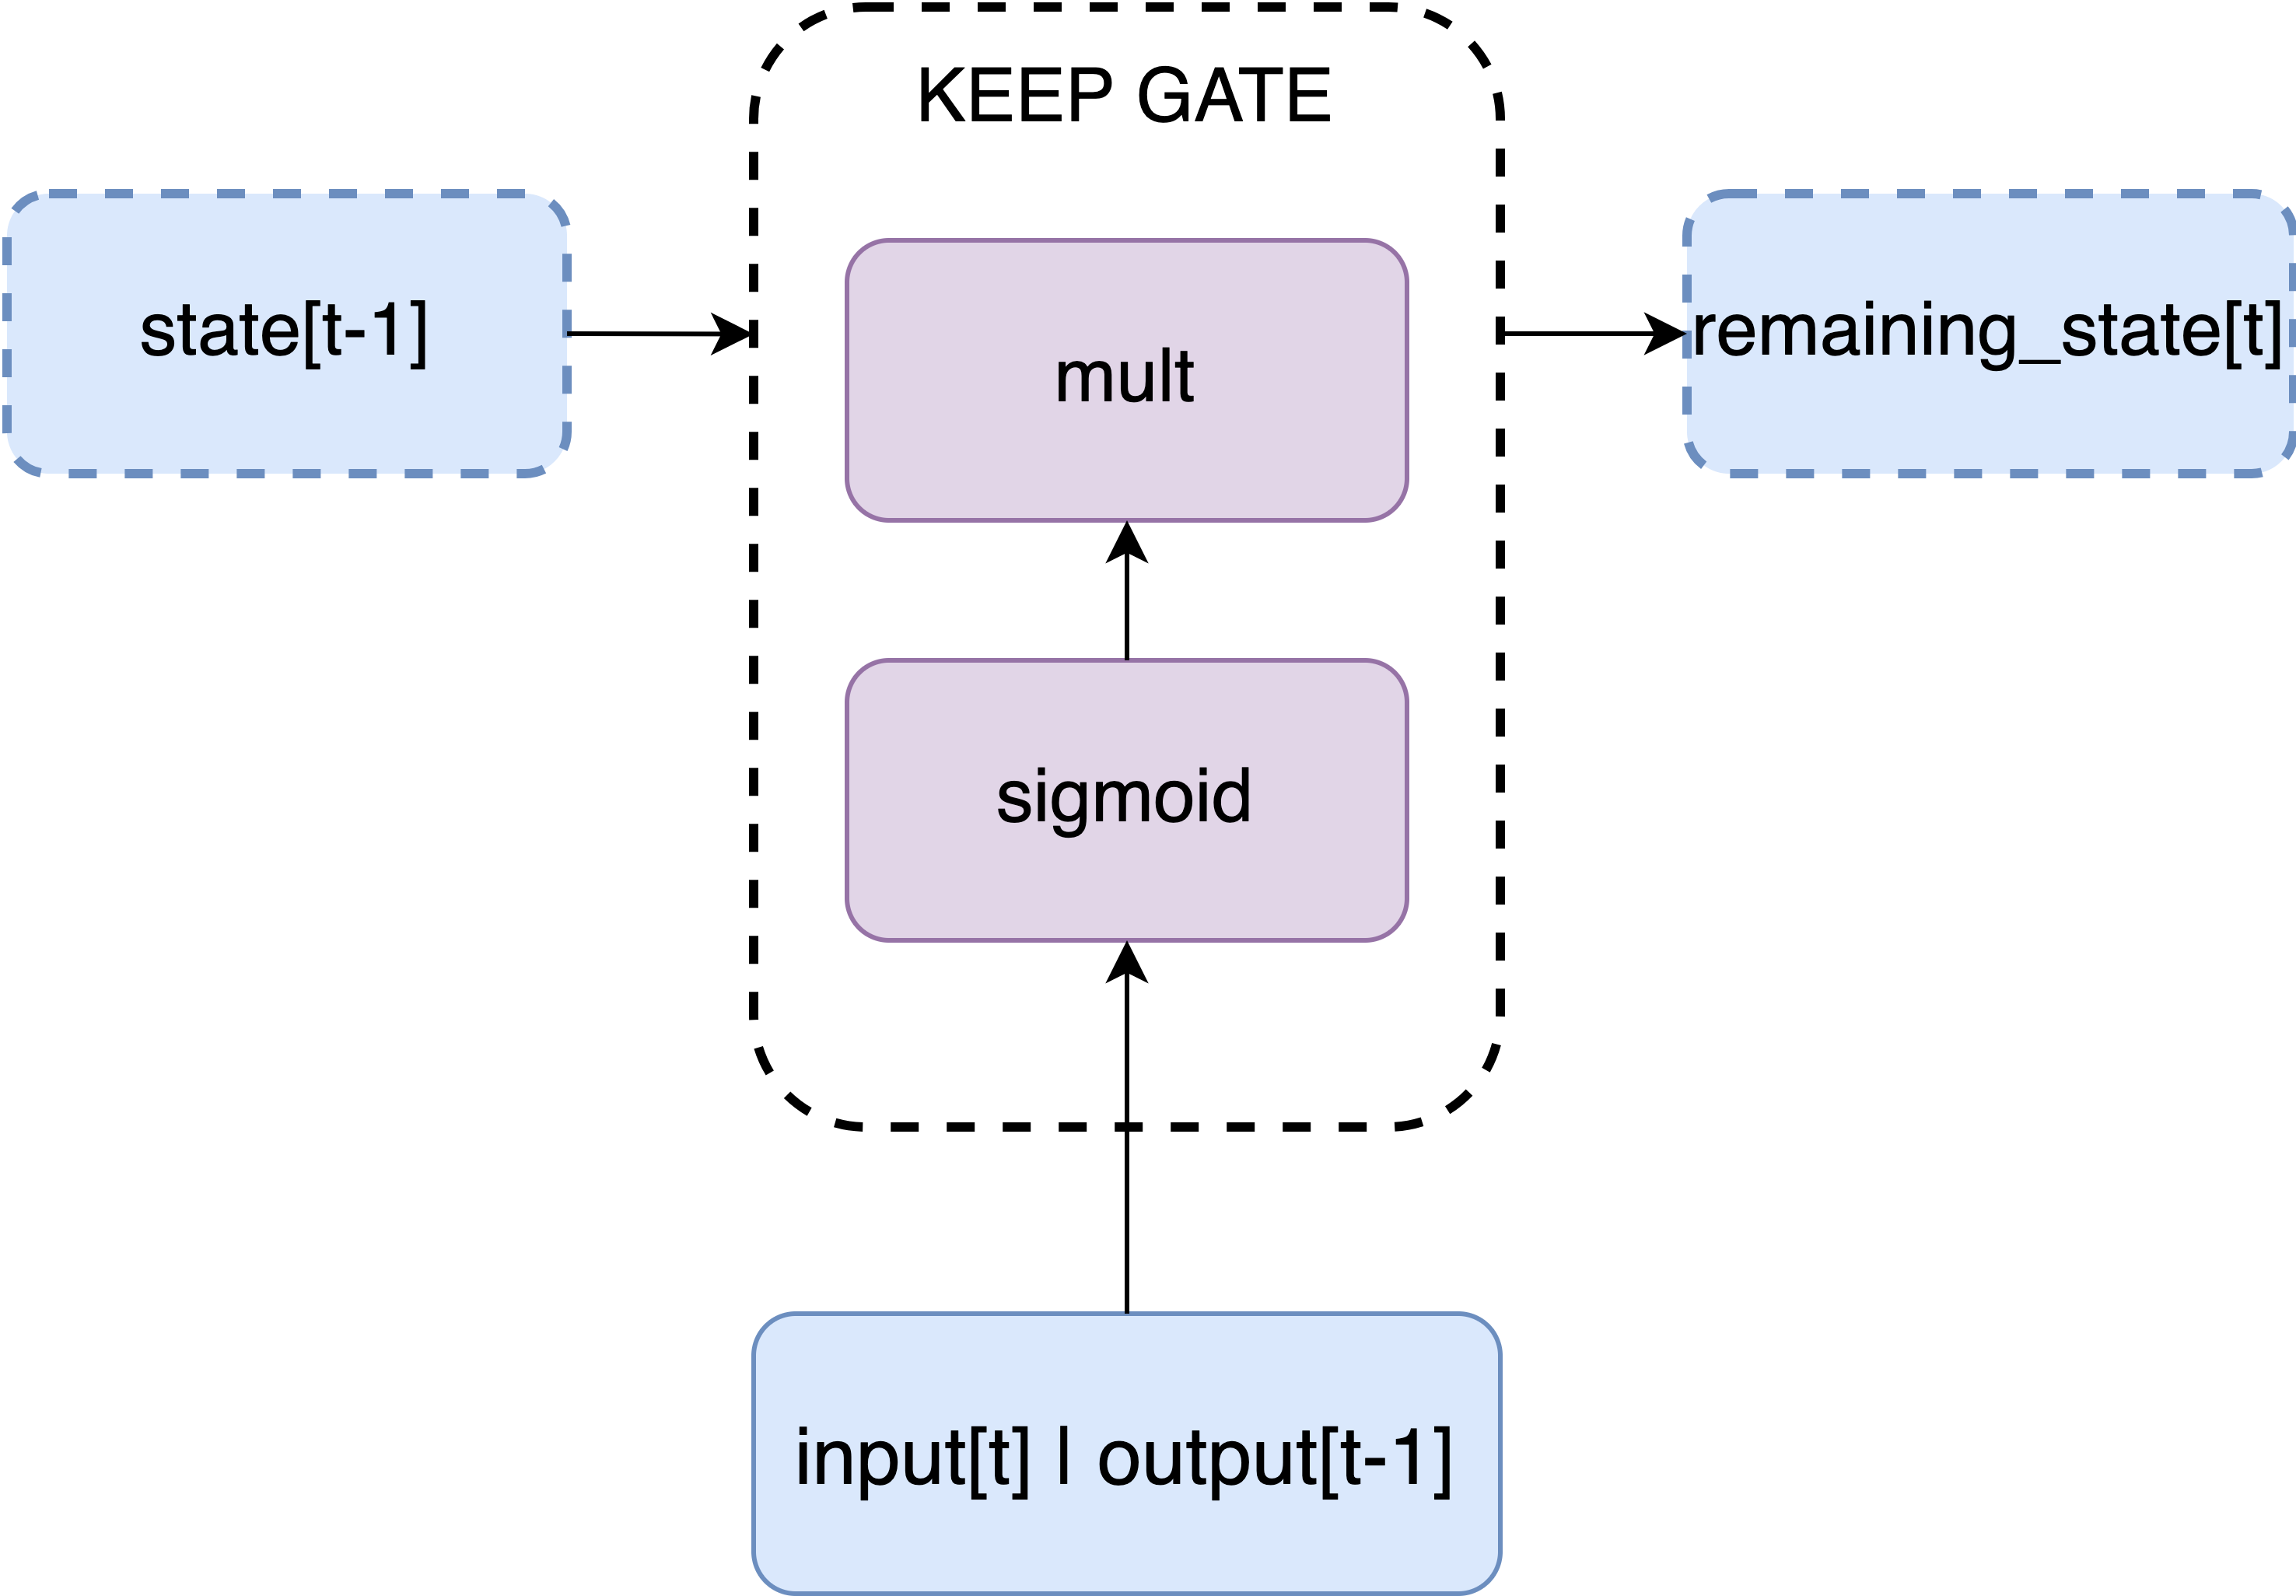
\includegraphics[width=0.85\textwidth]{Pictures/keep-gate.png}
	\hspace{1mm}
	\caption{Architecture of the keep gate of the LSTM unit.} 
	\label{fig:keep-gate}
\end{figure}

Once the LSTM knows which information is useful, it is ready to write into the memory state, shown in figure-\ref{fig:write-gate}. This part is handled by another LSTM unit called the write gate. The write gate's function can be broken down into two major parts. Figuring out what information to write into the state is the first step. This is computed by concatenating the output from the previous time-step along with the input of this time-step and applying a tanh activation to them. The second part involves figuring part which parts are relevant and need to be stored in the new state. A similar strategy is used as the keep gate by creating a bit vector and multiplying it with the intermediate tensor. The result is added with the output of the keep gate to create a new state. 
\begin{figure}[!h]
	\centering
	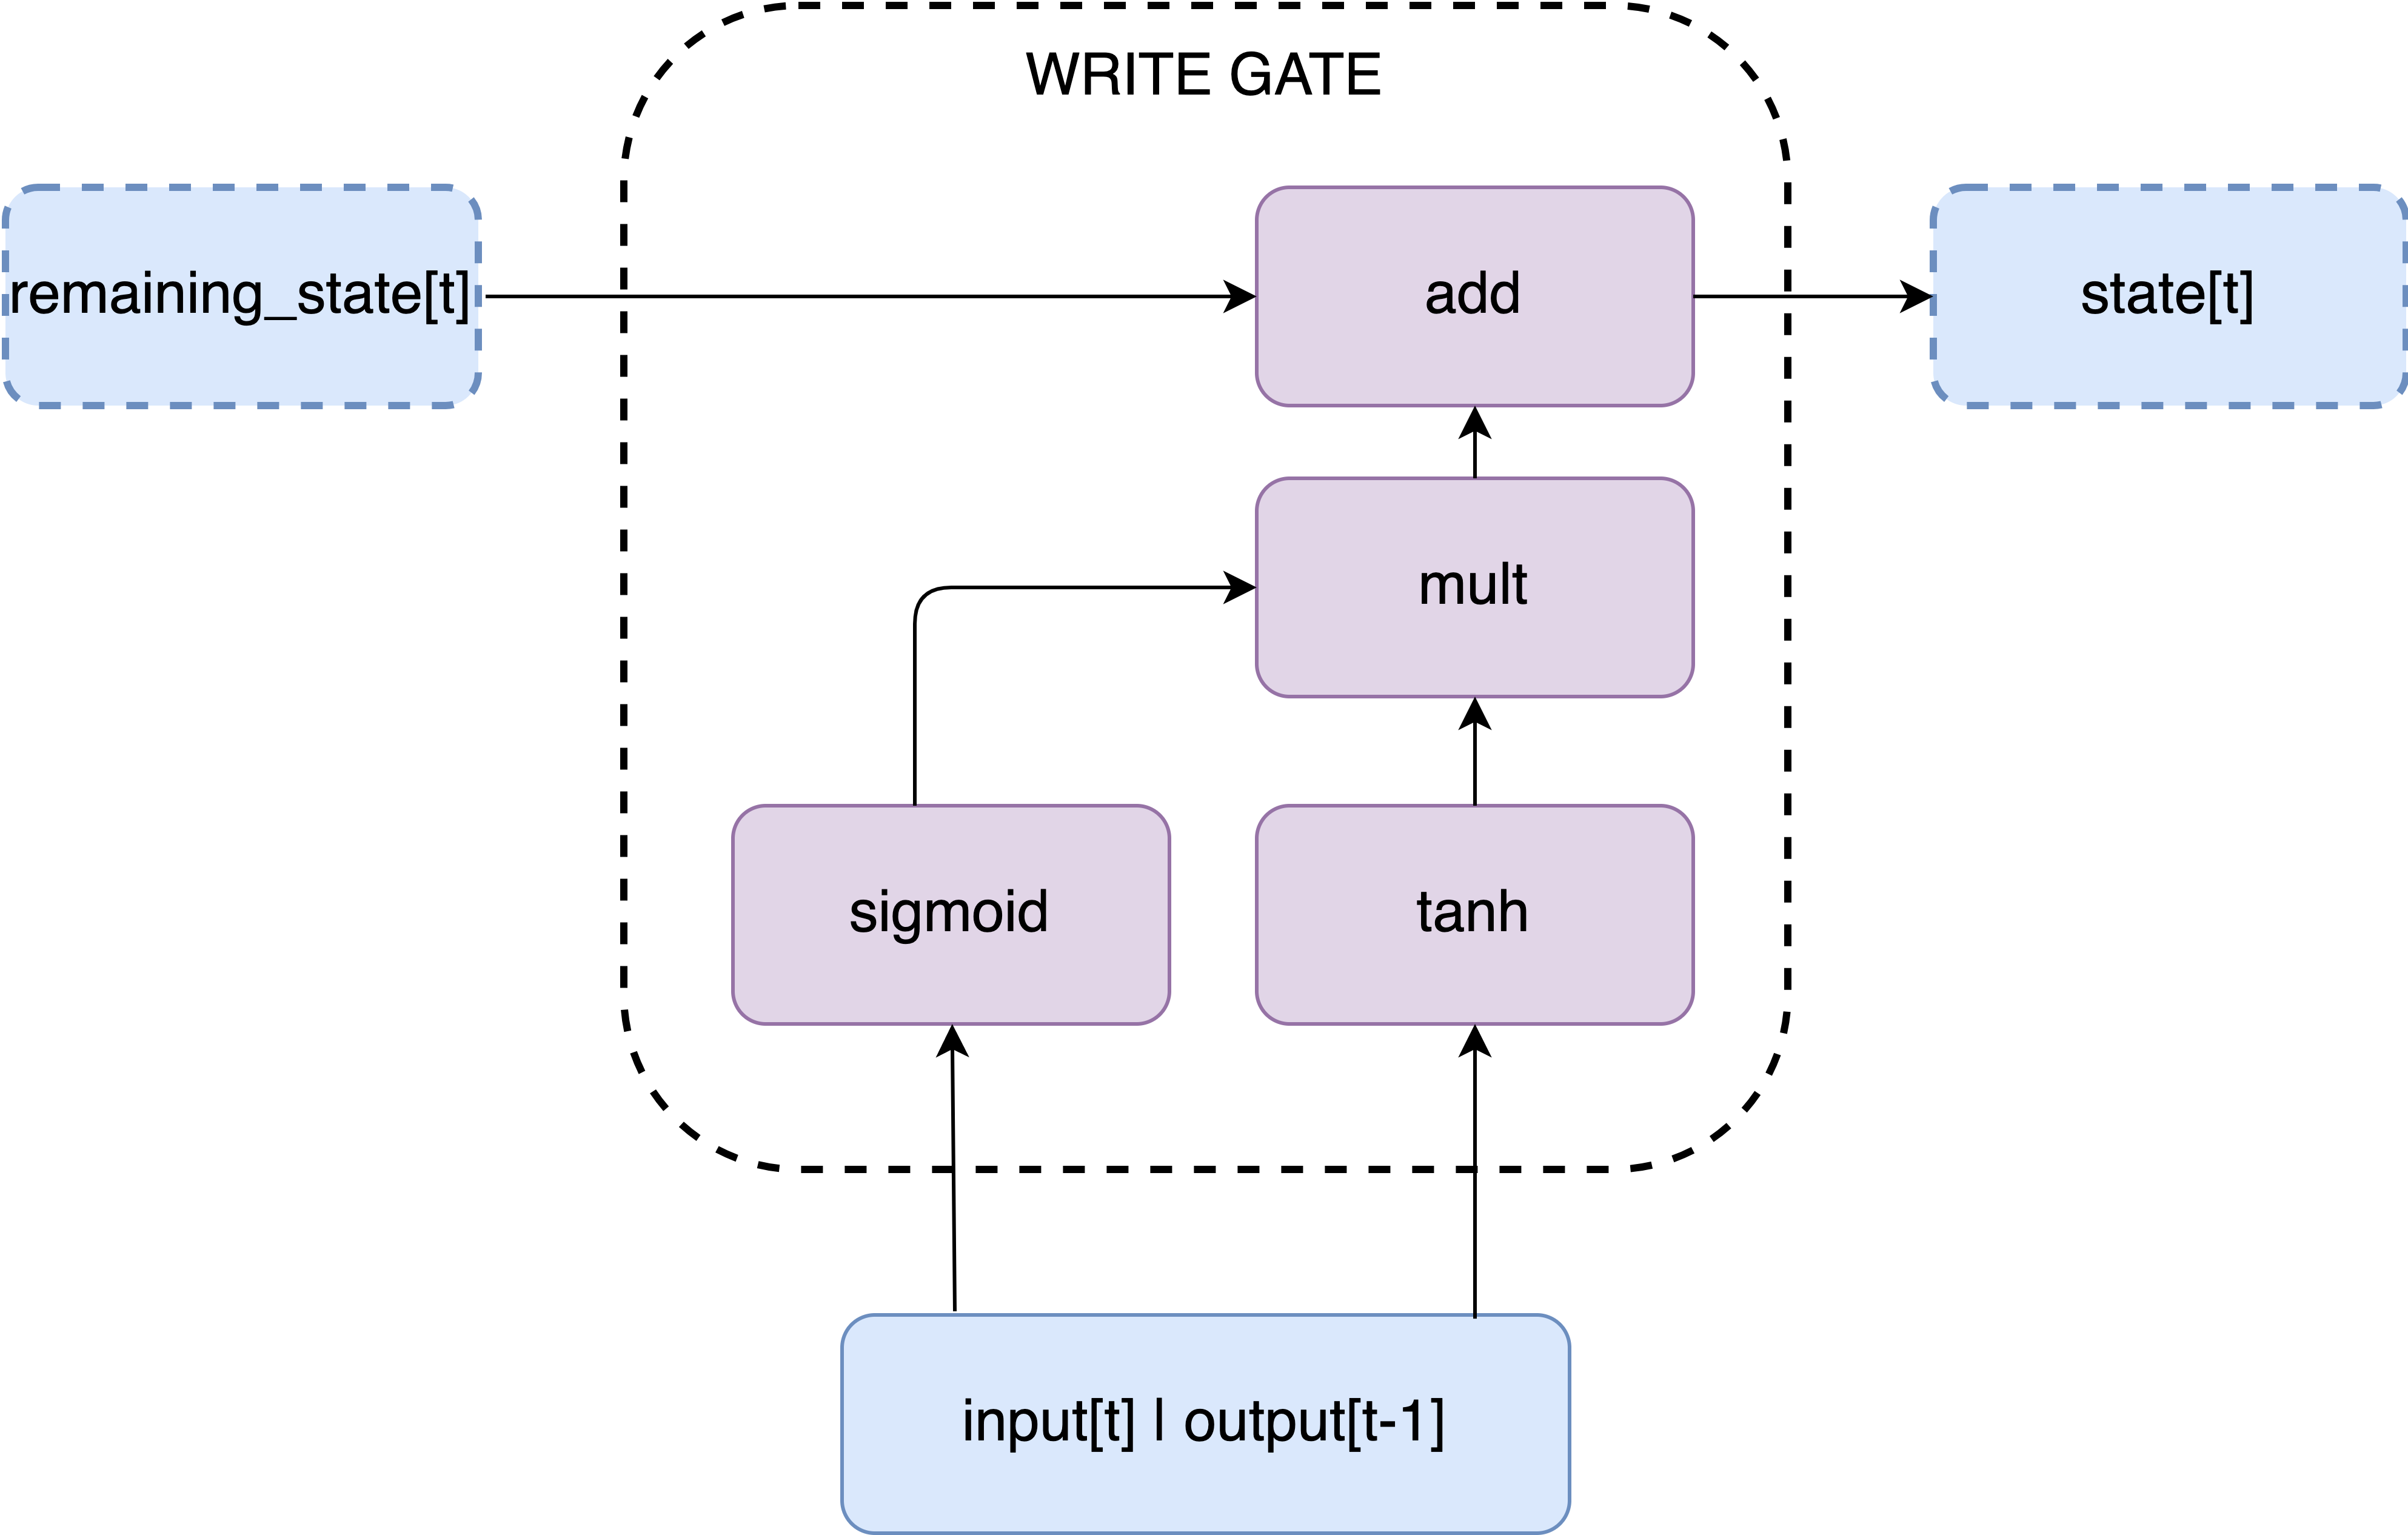
\includegraphics[width=0.85\textwidth]{Pictures/write-gate.png}
	\hspace{1mm}
	\caption{Architecture of the write gate of the LSTM unit } 
	\label{fig:write-gate}
\end{figure}

At the final step, the LSTM unit provide it's output. The structure of the output gate, shown in figure-\ref{fig:output-gate}, is similar to the write gate. Tanh activation is applied to the state vector to form an intermediate tensor. A sigmoidal layer is used to create the mask using the current input and previous output. The intermediate tensor is multiplied by the bit tensor(mask) to produce the final output.
\begin{figure}[!h]
	\centering
	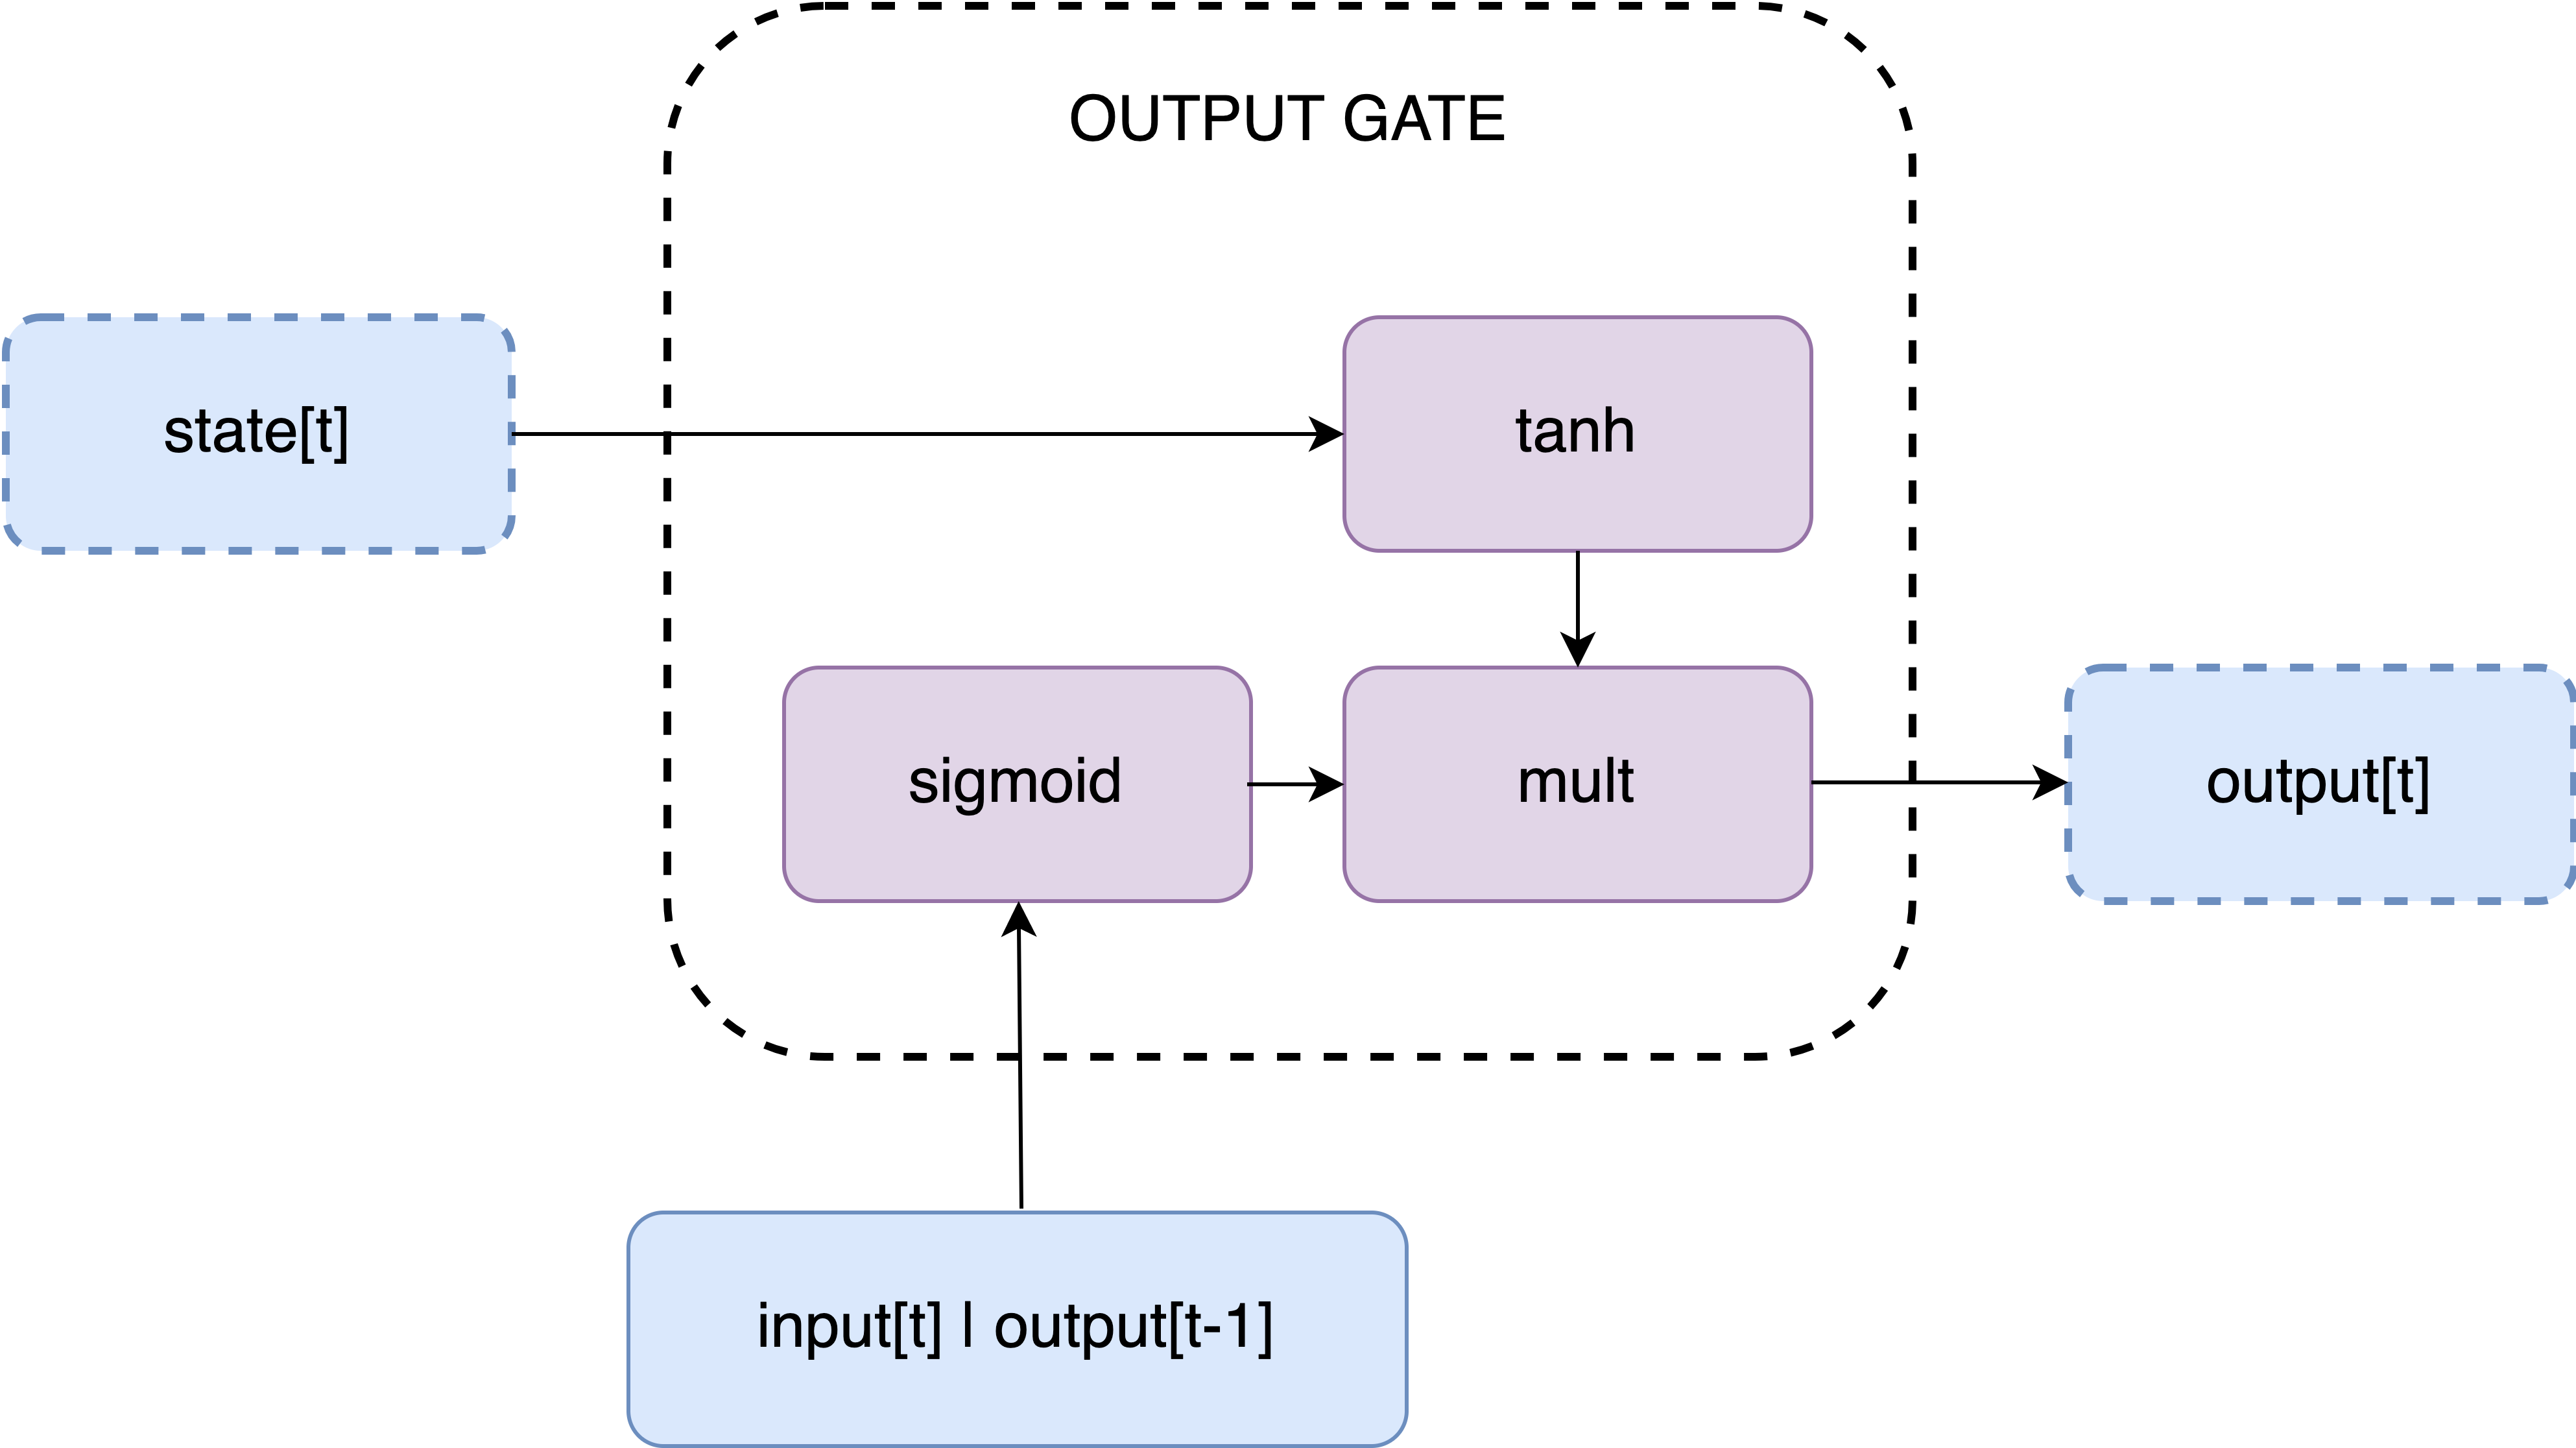
\includegraphics[width=0.85\textwidth]{Pictures/output-gate.png}
	\hspace{1mm}
	\caption{Architecture of the output gate of the LSTM unit.} 
	\label{fig:output-gate}
\end{figure}

The key equations involved in LSTM are given below where $\odot$ represents the Hadamard product, tanh is applied element-wise, $x_t, c_t$ and $h_t$ are the input, memory cell status and output of the LSTM at time $t$. $i_t, o_t$ and $k_t$ are the functional values of the write, output and keep gate. $W$s denote the weight matrix between the input and the gate and $b$s are the biases. 
\begin{equation}
    i_t = \sigma \left(W_{xi}x_t + W_{hi}h_{t-1} + W_{ci}\odot c_{t-1} + b_i \right) 
\end{equation}
\begin{equation}
    k_t = \sigma \left(W_{xk}x_t + W_{hk}h_{t-1} + W_{ck}\odot c_{t-1} + b_k \right)
\end{equation}
\begin{equation}
    c_t = f_t\odot c_{t-1} + tanh\left(W_{xc}x_t + W_{hc}h_{t-1} + b_c \right)
\end{equation}
\begin{equation}
    o_t = \sigma \left(W_{xo}x_t + W_{ho}h_{t-1} + W_{co}\odot c_{t-1} + b_o \right)
\end{equation}
\begin{equation}
    h_t = o_t\odot tanh(c_t)
\end{equation} 
% Chapter Template

\chapter{Model Development} % Main chapter title

\label{Chapter3} % Change X to a consecutive number; for referencing this chapter elsewhere, use \ref{ChapterX}

\lhead{Chapter 3. \emph{Model Development}} % Change X to a consecutive number; this is for the header on each page - perhaps a shortened title

%----------------------------------------------------------------------------------------
%	SECTION 1
%----------------------------------------------------------------------------------------

\section{Finite Element Modeling Framework}
%-----------------------------------
%	SUBSECTION 1
%-----------------------------------
\subsection{Microstructure Instantiation}
We have used an in-house MATLAB code to instantiate the 2D microstructures of a dual-phase (DP) steel comprising of ferrite and martensite phases. This code employs a weighted Voronoi tessellation algorithm for random positioning of grain centers within the simulation domain. The grain size distribution and volume fractions of the respective phrases are pre-defined based on experimental measurements. Figure-\ref{fig:grain-trans} shows the grain map of the microstructure generated by this algorithm. The desired mean radius $r_i$ and  volume fractions $V_i$ are given as inputs to the algorithm. The number of grains are calculated by the algorithm as $(Area\times V_i)/(\pi r_i^2)$. The sizes of these $n_i$ grains are generated randomly. The subscript $i$ has a value of 1 for ferrite and 2 for martensite. Details of the microstructure instantiation algorithm are given in Ref.  \cite{patra2015modeling}. The Trelis meshing software has been used to mesh the 2D microstructure with voxel-based elements. An element size of $0.25 \mu m$ is used to mesh the simulation domain of $100\times100 \mu m^2$.
\begin{figure}[!h]
	\centering
	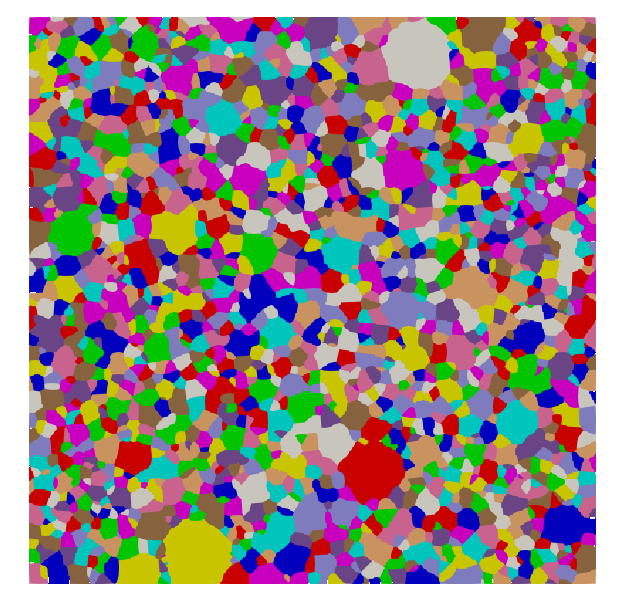
\includegraphics[width=0.65\textwidth]{Pictures/grain-trans.png}
	\hspace{1mm}
	\caption{Grain Map (colours are random and only to demarcate one grain from another)} 
	\label{fig:grain-trans}
\end{figure}
%-----------------------------------
%	SUBSECTION 2
%-----------------------------------
\subsection{Constitutive Model}
We have used a J2 plasticity constitutive modeling framework for the finite element (FE) computations. This framework is based on a finite deformation, dislocation density based model adapted from a crystal plasticity model previously used to model deformation behavior of various metallic systems \cite{POKHAREL2019201} \cite{THOOL2020102785}. While this is not a new feature of this work, details are provided here for completeness. 

In this framework, the deformation gradient is multiplicatively decomposed into the elastic and plastic parts: 
\begin{equation}
\boldsymbol{F} = \boldsymbol{F^e} \cdot \boldsymbol{F^p}
\end{equation}
where, $\boldsymbol{F^p}$ relates the reference configuration to an intermediate configuration and accounts for shear due to plastic deformation, while $\boldsymbol{F^e}$ relates the intermediate configuration to the current, deformed deformation and accounts for the rigid body rotation and elastic distortion. 
The elastic Green strain is given as:
\begin{equation}
\boldsymbol{E^e} = \frac{1}{2} (\boldsymbol{F^e}^T \cdot \boldsymbol{F^e} - \boldsymbol{I})
\end{equation}
Further, the second Piola-Kirchoff tensor is related to the elastic Green strain via the fourth rank elasticity tensor $\boldsymbol{C_o}$, i.e.,
\begin{equation}
    \boldsymbol{\sigma^{PK2}} = \boldsymbol{C_o} : \boldsymbol{E^e}
\end{equation}
The second Piola-Kirchoff tensor $\boldsymbol{\sigma^{PK2}}$ and the cauchy stress $\boldsymbol{\sigma}$
\begin{equation}
    \boldsymbol{\sigma} = \frac{\boldsymbol{F^e} \cdot \boldsymbol{\sigma^{PK2}} \cdot \left (\boldsymbol{F^e}\right)^T}{det\left (\boldsymbol{F^e}\right)}
\end{equation}
The von Mises effective stress, $\bar{\sigma}$ can be given in terms of the deviatoric part $\boldsymbol{S}$ of the Cauchy stress, i.e.,
\begin{equation}
    \boldsymbol{S} = dev(\boldsymbol(\sigma)) = \boldsymbol{\sigma} - \frac{\left (tr(\boldsymbol{\sigma}) \right )\boldsymbol{I}}{3}
\end{equation}
\begin{equation}
    \bar{\sigma} = \sqrt{\frac{3}{2}\boldsymbol{S}:\boldsymbol{S}}
\end{equation}
In J2 plasticity, the equivalent plastic strain rate $\dot{\bar{\epsilon}}^p$ is given as a function of the von Mises effective stress $\bar{\sigma}$. In this finite deformation framework, the plastic deformation gradient is related to the plastic velocity gradient as: $\boldsymbol{\dot{F}^p} = \boldsymbol{L^p} \cdot \boldsymbol{F^p}$, where $\boldsymbol{L^p}$ is the velocity gradient given by:
\begin{equation}
    \boldsymbol{L^p} = \dot{\bar{\epsilon}}^p \cdot \boldsymbol{N^p}
\end{equation}
where $\dot{\bar{\epsilon}}^p$ is the effective plastic strain, and $\boldsymbol{N^p}$ gives the direction of the plastic flow given by:
\begin{equation}
   \boldsymbol{N^p} =  \sqrt{\frac{3}{2}}\frac{\boldsymbol{S}}{\bar{\sigma}}
\end{equation}
The equivalent plastic strain rate is modelled using a Kocks-type activation enthalpy-driven flow rule:
\begin{equation}
\dot{\bar{\epsilon}}^p = \dot{\bar{\epsilon}}^p_o\exp\left(\frac{-\Delta F_g}{kT}\left(1 - \left(\frac{\sigma_{eff} - S_a}{S_t}\right)^p\right)^q\right)
\end{equation}
where, $\Delta F_g$ is the activation energy for dislocation glide, $S_a$ is athermal slip resistance, and $S_t$ is the thermal slip resistance, $p$ and $q$ are parameters used to model the shape of the activation enthalpy curve. The athermal slip resistance $S_a$ can be given by:
\begin{equation}
    S_a = \frac{h_p}{\sqrt{d}} + Gb\sqrt{q_p\rho}
\end{equation}
where, $h_p$ is the Hall-Petch hardening constant, $d$ is the grain size, $G$ is the shear modulus, $b$ is the Burgers vector, $q_p$ is the dislocation barrier strength and $\rho$ is the total dislocation density. $\rho$ is defined as the sum of immobile ($\rho_M)$ and mobile ($\rho_I)$ dislocation densities, i.e., 
\begin{equation}
    \rho = \rho_M + \rho_I
\end{equation}
The evolution of the dislocation densities with respect to time depends on the equivalent tensile plastic strain rate as:
\begin{equation}
\dot{\rho_M} = \frac{k_mul}{b}\sqrt{\Sigma\rho}|\dot{\bar{\epsilon}}^p| - \frac{2R_c}{b}\rho_M|\dot{\bar{\epsilon}}^p| - \frac{1}{b\lambda}|\dot{\bar{\epsilon}}^p|
\end{equation}
\begin{equation}
\dot{\rho_I} = \frac{1}{b\lambda}|\dot{\bar{\epsilon}}^p| - k_{dyn}\rho_I|\dot{\bar{\epsilon}}^p|
\end{equation}
where $\lambda = \frac{1}{\beta\sqrt{\rho}}$ is effective mean free path, $\beta$ is a constant associated with dislocation trapping, $k_{mul}$ is the dislocation multiplication rate constant and $R_c$ is the critical capture radius. The first term in Eq. 3.12 represents the multiplication of mobile dislocations at existing dislocations, while the second term represents the mutual annihilation of dislocation dipoles, and third term is the trapping of mobile dislocations at barriers. $k_{dyn}$ is the material constant associated with dynamic recovery of immobile dislocations due to thermally activated processes. The first term in Eq. 3.13 represents the rate at which mobile dislocations are trapped in barriers and become immobile, while the second term is the rate at which the immobile dislocations are annihilated due to dynamic recovery.

The constitutive model has been implemented as material model and interfaced with the open source finite element code, MOOSE \cite{permann2020moose}. The individual phases have been calibrated to the response of the ferrite and martensite phases based on available data in the literature. Further details and model parameters are given in Basu et al \cite{soudip}.

\subsection{Loading And Boundary Conditions}
A mesh size of $0.25 \mu m$ is used with a simulation domain size of $100\times100 \mu m^2$. The simulation domain has 40,000 elements.A generalized plane strain assumption is used in these essentially 2D simulations. The bottom face of the simulation domain is constrained in the y-direction, while the left face is constrained in the x-direction to resemble an axisymmetric model. The corner node common to both these faces is fully constrained to prevent rigid body motion. Displacement-controlled tensile loading is applied on the top face at a strain rate of $5\times10^{-3}s^{-1}$.
\begin{figure}[!h]
	\centering
	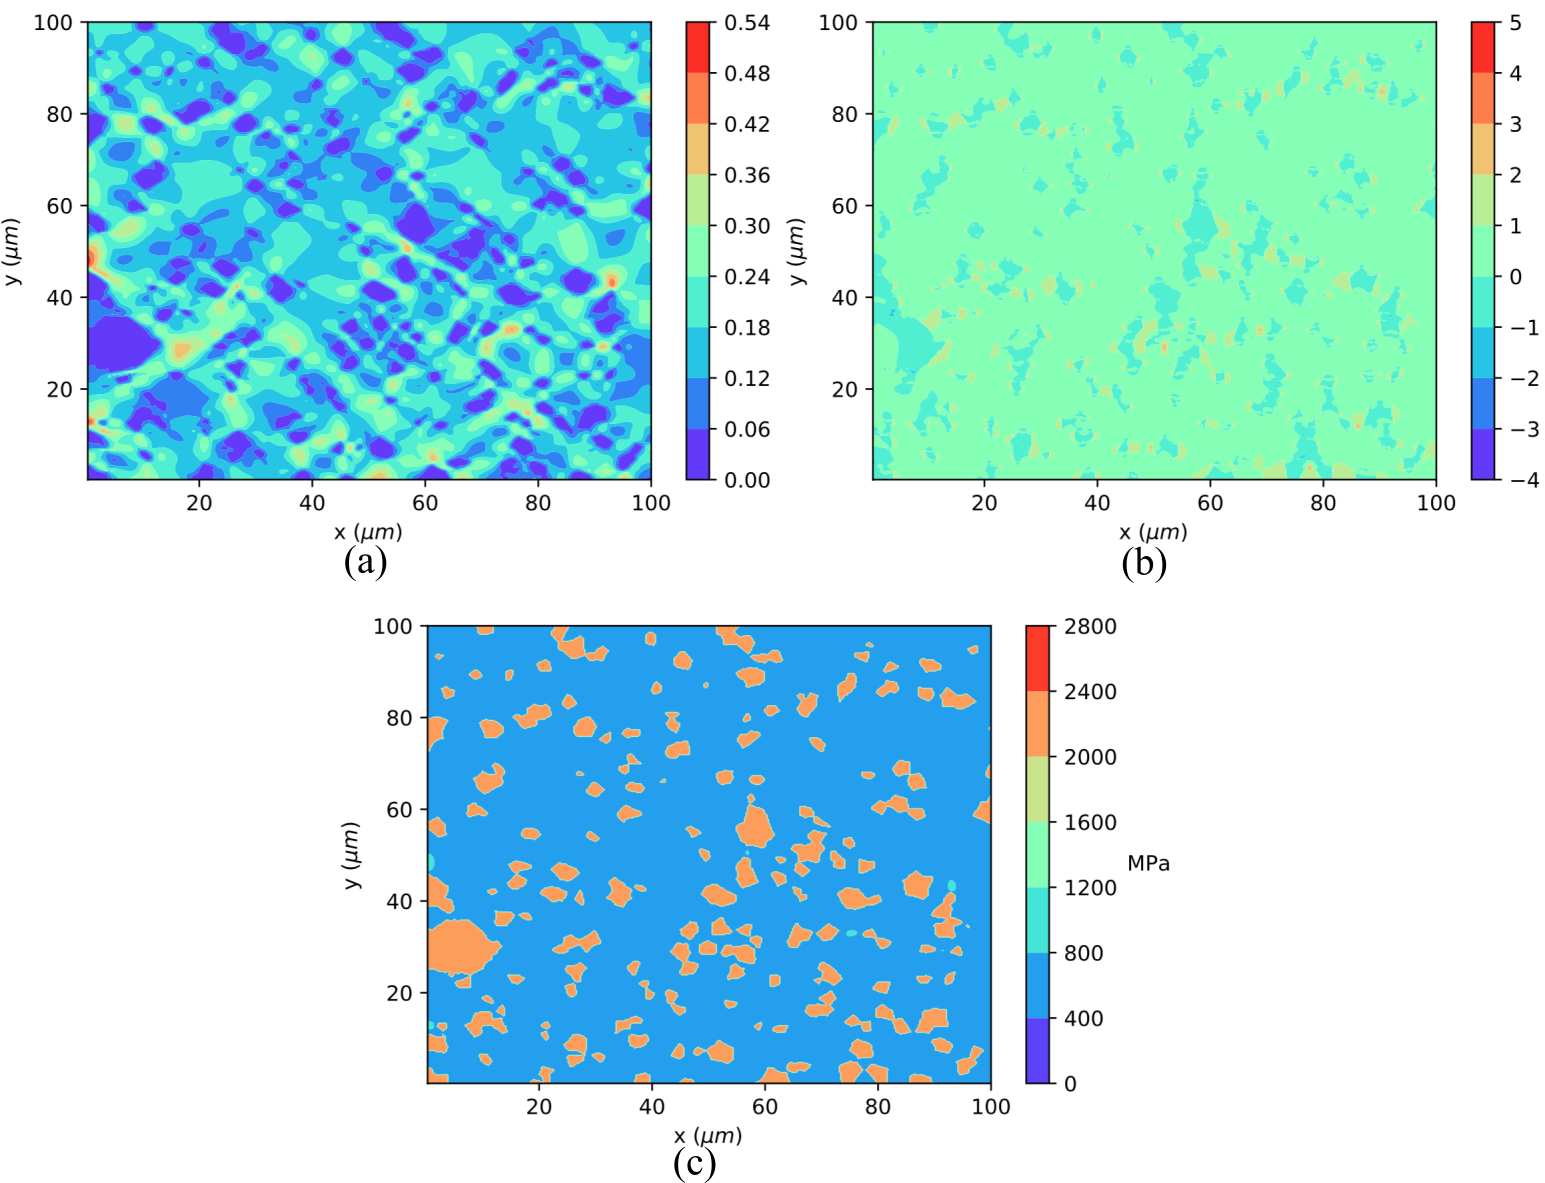
\includegraphics[width=\textwidth]{Pictures/result-fe.png}
	\hspace{1mm}
	\caption{Contour of (a) Effective Strain (b) Triaxiality (c) Vonmises Stress at the last time step} 
	\label{fig:exo-plots}
\end{figure}
\begin{figure}[!h]
	\centering
	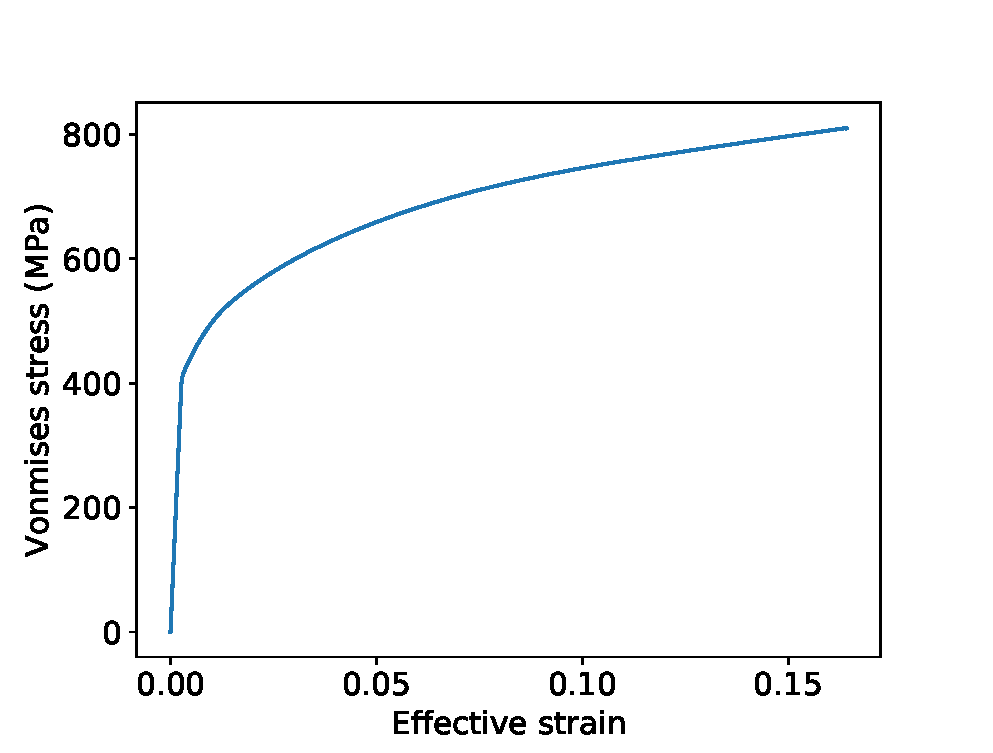
\includegraphics[width=0.8\textwidth]{Pictures/stress-strain.eps}
	\hspace{1mm}
	\caption{Effective strain vs Vonmises stress curve} 
	\label{fig:stress-strain}
\end{figure}

\section{Data Extraction from FE Results}
The simulation results of the FE model are output to an EXODUS data file. The EXODUS format is a binary file which is used for FE pre- and post-processing. Data used to define the finite element mesh, along with both the boundary conditions and load application points are includes in the file. The EXODUS format is advantageous as it combines the mesh data as well as the results data in a single file. This assures the user that the results are consistent with the model \cite{mills1988exodus}. However, to access this data in a usable and easily interpretable way, special software are used. For the purpose of this project, we have used the  Sandia Engineering Analysis Code Access System (SEACAS) developed by Sjaardema \cite{seacas}. The library consists of packages which can convert an EXODUS file's data to different formats like text file and MATLAB data files. The Python package has been used for this project which makes reading the data from an EXODUS file viable through a python script. The package provides a number of predefined functions to extract different information from the EXODUS file. Using these functions, we have extracted all the data from the EXODUS file to a csv format. The csv format has all the element variable values at every time-step for every element. The script is written in Python 2.7.17 and take approximately 10 minutes to execute. The time taken by the script varies with the mesh size and number of variables in the exodus file.   

\section{Machine Learning Framework}
\subsection{ANN Model}
At the basic level, the process of developing an ANN model (or any learning model) has two primary steps. First one being, selecting the relevant, representative and compact set of  features and then developing a relation between them to get the desired result. Elimination of irrelevant features and selection or relevant ones is one of the central tasks in machine learning \cite{blum1997selection}. In this context, it has been assumed that the observed heterogeneity in deformation is due to the underlying heterogeneity of the microstructure. The features of interest are highlighted in the Table \ref{tab:feature-table}. 
\begin{table}
\begin{center}
\begin{tabular}{|c|c|}
\hline
Feature & Description \\
\hline
\textit{x} & x-coordinate of the element \\
\hline
\textit{y} & y-coordinate of the element \\
\hline
\textit{p} & Phase to which the element belongs (ferrite or martensite) \\
\hline
\begin{math}{\epsilon_{app}}\end{math}& Applied (or nominal) strain \\
\hline
\end{tabular}
\end{center}
\caption{\label{tab:feature-table}Selected feature names and descriptions.}
\end{table}

The output variables of interest are effective strain, ${\bar{\epsilon}}$, von Mises effective stress, $\bar{\sigma}$, and stress triaxiality ratio. While, effective strain and effective stress can be correlated with plastic deformation in the respective phases, the stress triaxiality ratio (given as the ratio of the mean stress over the von Mises effective stress) provides a measure of the development of multi-axial stress states that may contribute to eventual failure initiation in the material. In the present context, the ferrite-martensite interfaces are potential sites for failure initiation in DP steels and hence it is pertinent to be able to predict the stress triaxiality ratio as well. For each element, ${\bar{\epsilon}}$, $\bar{\sigma}$ and triaxiality ratio are recorded at applied strain intervals of $0.01$. The simulation is run up to $0.15$ nominal strain, thus providing us a total of fifteen datasets at $0.01$ nominal strain intervals. The mesh consists of $400\times400$ elements, making the length of every feature and target variable vector $2,400,000$. Thus, the shape of our input is $2,400,000\times4$ and the corresponding shape of output is $2,400,000\times3$. 

Note that feature selection depends on the output variables of interest and may vary if it is desired to output a different set of variables. Mangal and Holm \cite{MANGAL2018122} provide a detailed study of the performance of neural network models with different input features for a crystal plasticity model. In the context of a J2 plasticity model, we assume the features given in Table \ref{tab:feature-table} to be the most relevant for the present problem.

Any ANN model is very sensitive to the magnitude of the training data. Given that we are interested in strains and stresses, whose magnitudes are generally many orders apart, all the data has been normalized within the range $[0,1]$ in the present work. The normalised values $x_i^n$ for any training variable $x_i$ are calculated as:
\begin{equation}
    x_i^n = \frac{x_i - x_{min}}{x_{max} - x_{min}}
\end{equation}
In this work, the mean-squared error function (MSE) has been used and the sigmoid function has been employed as the activation function for every neuron. The completed training and model development process has been performed using python and Keras with a Tensorflow backend. Data splitting is another important task during data splitting where hold-out validation is employed to ensure generalisation \cite{may2010data}. The dataset is split into training ($80\%$) and testing ($20\%$) datasets. The training data is used to for training and learning of the ANN, whereas the testing dataset is used to check the accuracy of the fitted parameters. The validation dataset is unseen by the ANN model, therefore predictions made by the model on the validation dataset represents the degree to which the model generalizes over our data. A number of networks were trained on this data with different architectures. The network which performed relatively better than others consisted of 4 inputs, 3 hidden layers and 3 outputs. The training of the neural network is performed over 5 epochs and takes 106 minutes to train. 
\begin{figure}[!h]
	\centering
	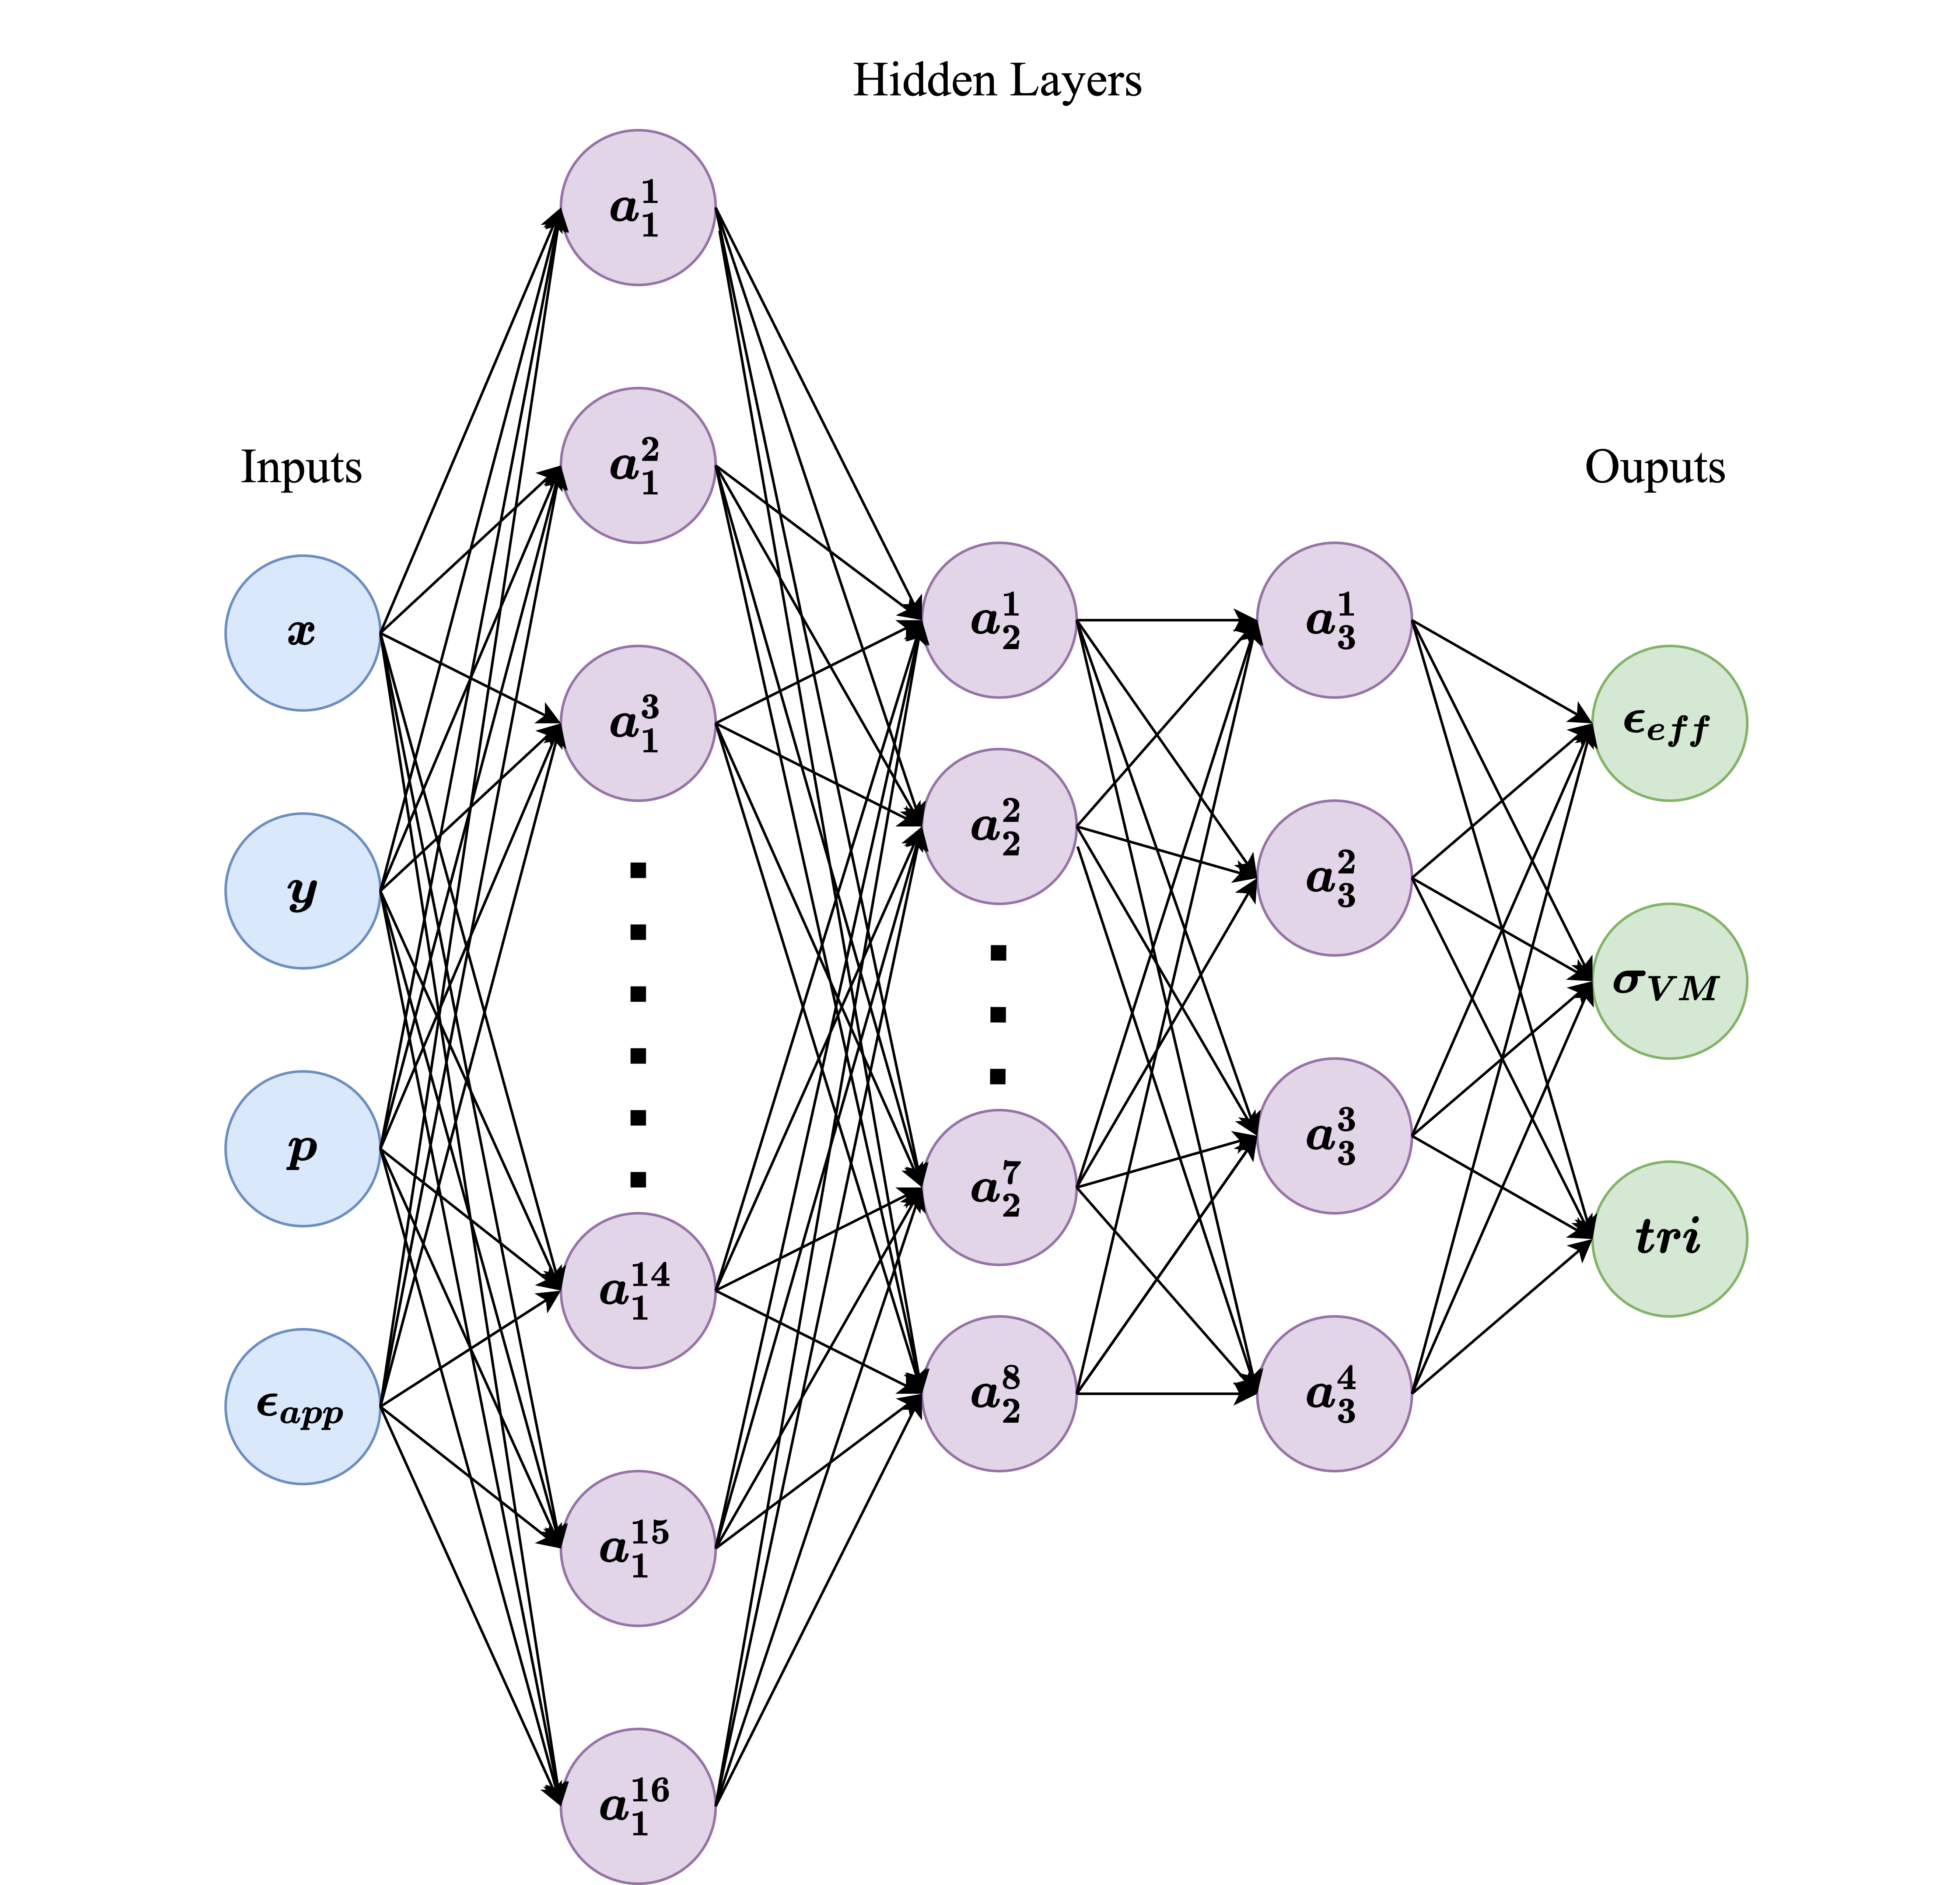
\includegraphics[width=0.9\textwidth]{Pictures/my-ann.png}
	\hspace{1mm}
	\caption{Schematic of proposed ANN architecture} 
	\label{fig:my-ann}
\end{figure}
\begin{figure}[!h]
	\centering
	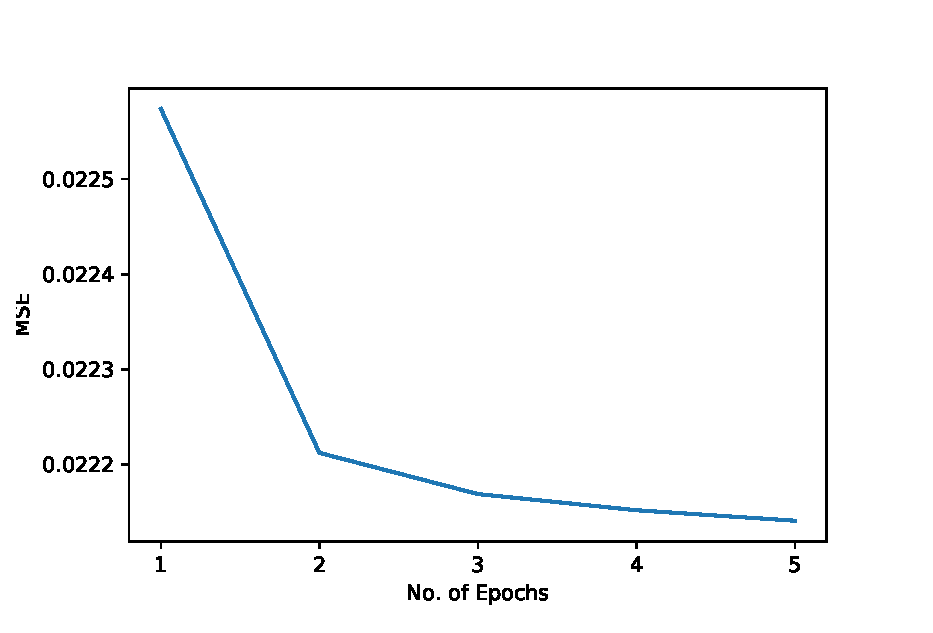
\includegraphics[width=0.8\textwidth]{Pictures/training_process.eps}
	\hspace{1mm}
	\caption{Learning curve showing the evolution of MSE loss over training data-set} 
	\label{fig:ann-training}
\end{figure}

\subsection{LSTM Model}
LSTMs have shown great accuracy in predicting sequence and time series data. The evolution of local strain distribution can be formulated as a sequence modeling problem. As with ANN, we are focusing on three output variables in our model, namely, effective strain, ${\bar{\epsilon}}$, von Mises effective stress,  $\bar{\sigma}$, and stress triaxiality ratio. For every element, the values of these variables are recorded for every $0.01$ nominal strain interval. As mentioned previously, the simulation is run till $0.15$ nominal strain and hence our data contains $15$ strain steps. Each element is associated with 3 sequences of length 15, and as there are $400\times400$ elements the total number of series or model predicts is $400\times400\times3$. For a given strain step $t$, $400\times400\times3$ length vector $\boldsymbol{X_t}$ is input to the LSTM model and used to predict the output vector, $\boldsymbol{Y_t}$ which consists of values at the next strain step in the series $X_{t+1}$. The structure of the data can be understood better through the Table \ref{tab:lstm-data-table}. All data was normalized within the range of $[0,1]$. The data was split into training ($70\%$) and test ($30\%$) datasets, meaning the training dataset consisted of only the first $10$ strain steps. The model was trained using the training dataset run over 300 epochs. The last $5$ strain steps were used to check how well the model performs on data it has not seen before. The model consists of $8$ LSTM layers with $200$ neurons in each layer. The activation function employed in this case is ReLU. The choice of activation function is driven by the reduction in MSE over the epochs. Figure \ref{fig:diff-activation-lstm} shows the performance of different activation functions while training the same dataset. The number of layers and neuron are the same for these model, only the variation with activation function is checked for. It can be observed that ReLU performs better than the other two activation functions by at least two orders of magnitude of MSE.

\begin{table}
\begin{center}
\begin{tabular}{|c|c|}
\hline
Input (\begin{math}\boldsymbol{X}\end{math})&Output (\begin{math}\boldsymbol{Y}\end{math}) \\
\hline
\begin{math}\boldsymbol{X_1}\end{math}& \begin{math}\boldsymbol{X_2}\end{math} \\
\begin{math}\boldsymbol{X_2}\end{math}& \begin{math}\boldsymbol{X_3}\end{math}  \\
\begin{math}\boldsymbol{X_3}\end{math}& \begin{math}\boldsymbol{X_4}\end{math} \\
. & . \\
. & . \\
. & . \\
. & . \\
\begin{math}\boldsymbol{X_{10}}\end{math}& \begin{math}\boldsymbol{X_{11}}\end{math} \\
\hline
\end{tabular}
\end{center}
\caption{\label{tab:lstm-data-table}Training data format for LSTM.}
\end{table}

\begin{figure}[!h]
	\centering
	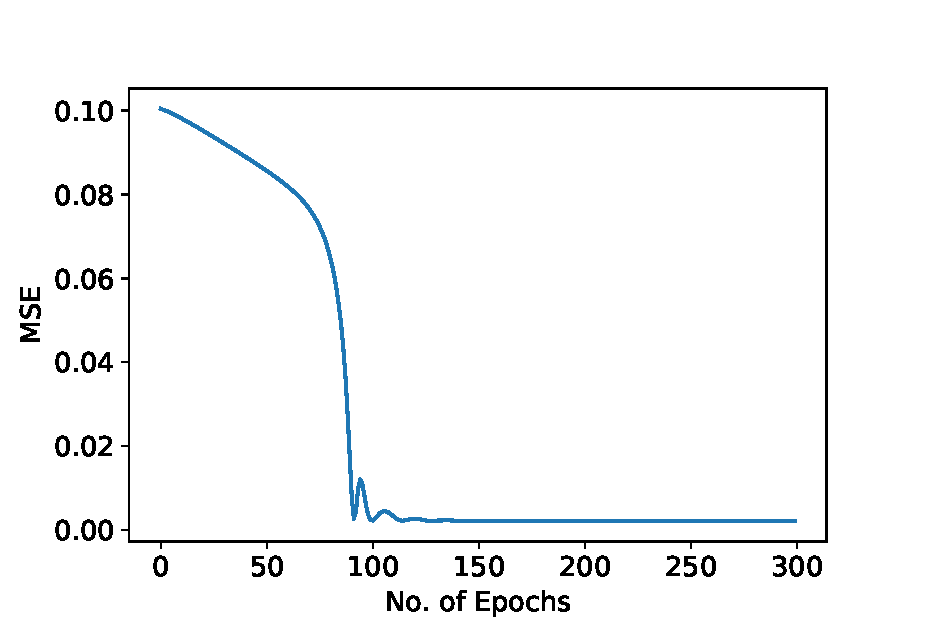
\includegraphics[width=0.7\textwidth]{Pictures/lstm-res/lstm-tanh_loss.eps}
	\hspace{1mm}
	\caption{Learning curve showing the evolution of MSE loss over training data-set.} 
	\label{fig:ann-training}
\end{figure}

\begin{figure}[!h]
	\centering
	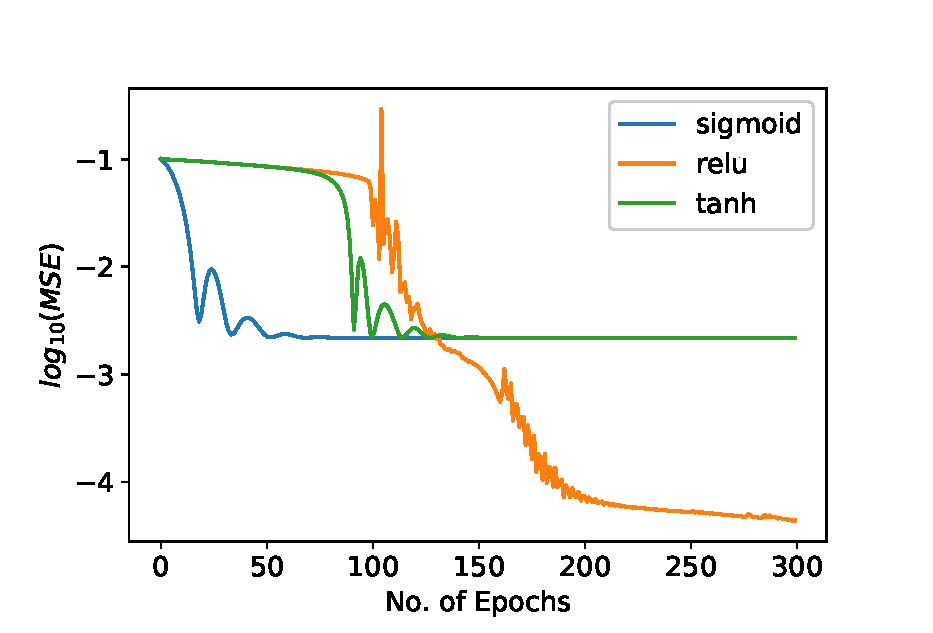
\includegraphics[width=0.7\textwidth]{Pictures/lstm-res/lstm-sctivations_log.eps}
	\hspace{1mm}
	\caption{Comparative study of MSE obtained in training models with different activation functions} 
	\label{fig:diff-activation-lstm}
\end{figure}
\begin{sidewaysfigure}[ht]
	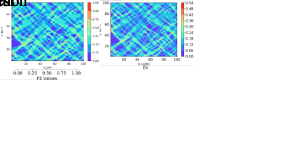
\includegraphics[width=0.95\textwidth]{Pictures/lstm-res/flow-purple.png}
	\hspace{1mm}
	\caption{Schematic representation of the proposed ML framework} 
	\label{fig:flow-chart}
\end{sidewaysfigure}
\iffalse
Along with a vanilla LSTM, two modification of LSTMs were also trained:
\begin{enumerate}
\item \textbf{Auto-regressive}: The training of procedure of this LSTM is similar to that of a vanilla LSTM, however the difference arises in the way predictions are made. For a regular LSTM, to predict the value of a sequence at time $t$ one would need to know all the true values till time $t-1$ and so on for $t+1$. In an auto-regressive methodology once an initial prediction is made using the available sequence data, all further predictions are made using this initial prediction. Say for example, a prediction is made for time $t$. To predict $t+1$ time-step, instead of using the input sequence data we use this predicted value at time $t$. This enables our LSTM to predict sequence values further into the future without requiring input data up to the penultimate step.
\item \textbf{LSTM-FC}: This kind of model consists two major components: (1) A long-short term memory based temporal simulator to model the local strain developments and (2) A neural network to capture the spatial dependencies of strain between a central element and it's neighbours. The LSTM capable of handling long term dependencies handles only the temporal information in the data, and the spatial information is incorporated using a fully connected neural network. The neural network is trained such that given 8 neighbouring elements' property values it can make predictions  for the central element. 
\end{enumerate}
\fi
% Chapter Template

\chapter{Results and Discussion} % Main chapter title

\label{Chapter4} % Change X to a consecutive number; for referencing this chapter elsewhere, use \ref{ChapterX}

\lhead{Chapter 4. \emph{Results and Discussion}} % Change X to a consecutive number; this is for the header on each page - perhaps a shortened title

%----------------------------------------------------------------------------------------
%	SECTION 1
%----------------------------------------------------------------------------------------

\section{Artificial Neural Network (ANN) Results}
The relationship between the microstructure and mechanical behaviour of DP steels is extremely complex. Successful implementation of an ANN model would have helped understand these complex relations and helped in predicting experimental behavior of other heterogeneous systems. For assessing our model's predictive capabilities over three different variables simultaneously, a metric is used to estimate how well the model performs for each of these variables. For this purpose, we calculate the coefficient of determination, $R^2$. $R^2$ represents the proportion of variance that has been explained by the independent variables in the model. It provides an indication of goodness of fit and therefore a measure of how well unseen samples are likely to be predicted by the model, through the proportion of explained variance. Best possible score is 1.0 and it can be negative (because the model can be arbitrarily worse). This metric is given by the following equation:
\begin{equation}
    R^2(y, \hat{y}) = 1 - \frac{\sum_{i=1}^{n} (y_i - \hat{y}_i)^2}{\sum_{i=1}^{n} (y_i - \bar{y})^2}
\end{equation}
where $y$ is the actual output (true value) and $\hat{y}$ is the prediction made by the ANN model. For a model with $100\%$ accuracy then $y_i = \hat{y}_i)$ for all $i's$ making $R^2 = 1$, which indeed is the best case scenario. 

A number of neural network architectures were trained and their $R^2$ and mean squared error values were recorded for a comparative parametric study. The following table shows the results that were obtained along with the time taken to train each model. 

\begin{table}
\begin{center}
\begin{tabular}{|c|c|c|c|c|c|c|}
\hline
Layers & Architecture & MSE & Time & \multicolumn{3}{c|}{$R^2$} \\
\hline
&(Neurons in every layer) & & (hrs)& ${\bar{\epsilon}}$ & $\bar{\sigma}$ & tri \\
\hline
2 & 8,4 & 0.0221 & 1.44 & 0.55 & 0.16 & 0.7 \\
3 & 16,8,4, & 0.0221 & 1.76 & 0.55 & 0.16 & 0.07 \\
4 & 32,16,8,4 & 0.0221 & 1.78 & 0.55 & 0.17 & 0.06 \\
5 & 64,32,16,8,4 & 0.0222 & 1.82 & 0.55 & 0.15 & 0.05 \\
6 & 128, 64,32,16,8,4 & 0.0266 & 1.87 & 0.16 & 0.13 & 0.02 \\
7 & 256,128,64,32,16,8,4 & 0.0290 & 3.47 & $<0$ & $<0$ & $<0$ \\
8 & 512,256,128,64,32,16,8,4 & 0.0290 & 4.59 & $<0$ & $<0$ & $<0$ \\
9 & 1024,512,256,128,64,32,16,8,4 & 0.0289 & 7.32 & $<0$ & $<0$ & $<0$ \\
11 & 1024,1024,512,512,256,128,64,32,16,8,4 & 0.0290 & 20.24 & $<0$ & $<0$ & $<0$ \\
\hline
\end{tabular}
\end{center}
\caption{\label{tab:diff-ann-table}Study of accuracy of models with different depths and neurons.}
\end{table}

As can be clearly seen from the table, the model is unable to make the predictions successfully. The MSE is very high and the $R^2$ values too low. For the model to be acceptable, the MSE values should have been in the range of $10^{-4} - 10^{-5}$ and $R^2$ values should be above $0.80$. All the above simulations have run for 5 epochs. Increasing the epochs is usually accompanied by a decrease in error. However, even after increasing to 20 epochs, the $R^2$ values did not improve. The first architecture in Table \ref{tab:diff-ann-table} was trained for 20 epochs. The MSE reduced to 0.0216, but $R^2$ values remained approximately the same. Increasing the epochs increased the training time to 8.5 hours without yielding any significant results.  Increasing the dept and complexity of the network is another way to increase the accuracy. However, as can be seen from the table, the MSE and $R^2$ values actually worsen as the number of hidden layers are increased beyond 4. Another major drawback in the ANN model is the limited dataset we are using to train it. The data consists of only discrete data at $0.01$ strain intervals. If instead, we trained our data to smaller strain intervals of the FE simulations, the results would be perhaps better, albeit at the cost of significant training times.

ANN predicted values are plotted in Figure \ref{fig:exp_pred_ann} against the ground truth values to better visualize the performance of our model. Note that all results are plotted on the normalized scales. For an ideal case, all the data points would lie as close to the $y=x$ line.
\begin{figure}[!h]
	\centering
	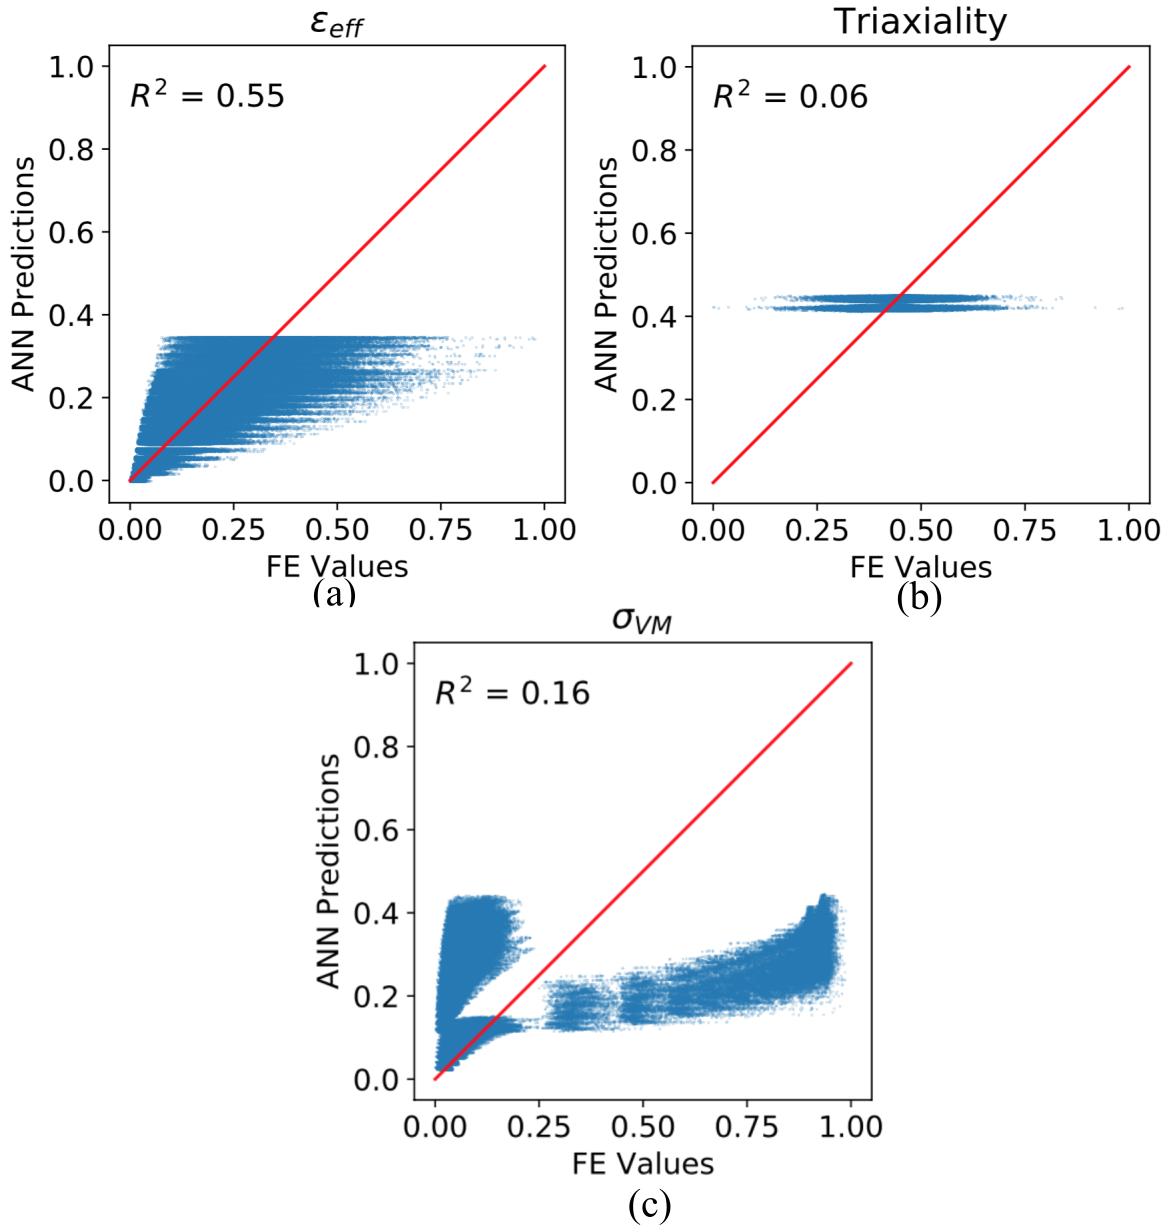
\includegraphics[width=0.9\textwidth]{Pictures/ann-res/final-ann-bitmap.png}
	\hspace{1mm}
	\caption{Plot of ANN predicted values vs FE values for (a) effective strain, (b) stress triaxiality ratio, and (c) von Mises effective stress. Note that all the variables are normalized.} 
	\label{fig:exp_pred_ann}
\end{figure}
A separate model was also trained to predict only one variable, effective strain. The architecture was kept the same, and the results showed an improvement in the $R^2$ value. We can conclude that predicting multiple variables using a single ANN leads to inaccuracy. Figure-\ref{fig:r2-ann} shows the $R^2$ values and figure-\ref{fig:ann-contours} shows the contour plots of ANN predicted value as compared to the true values. The numerical value of the predictions is quite inaccurate however, the ANN model has been able to locate some hotspots. 
\begin{figure}[!h]
	\centering
	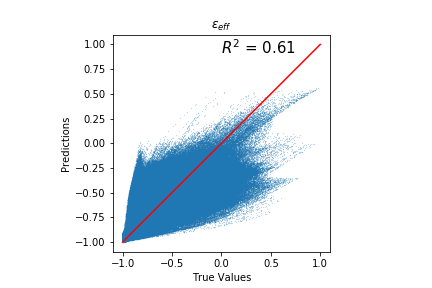
\includegraphics[width=0.9\textwidth]{Pictures/strain_eff_pred_exp.png}
	\hspace{1mm}
	\caption{Plot of ANN predicted values vs FE values for effective strain trained alone} 
	\label{fig:r2-ann}
\end{figure}

\begin{figure}[!h]
	\centering
	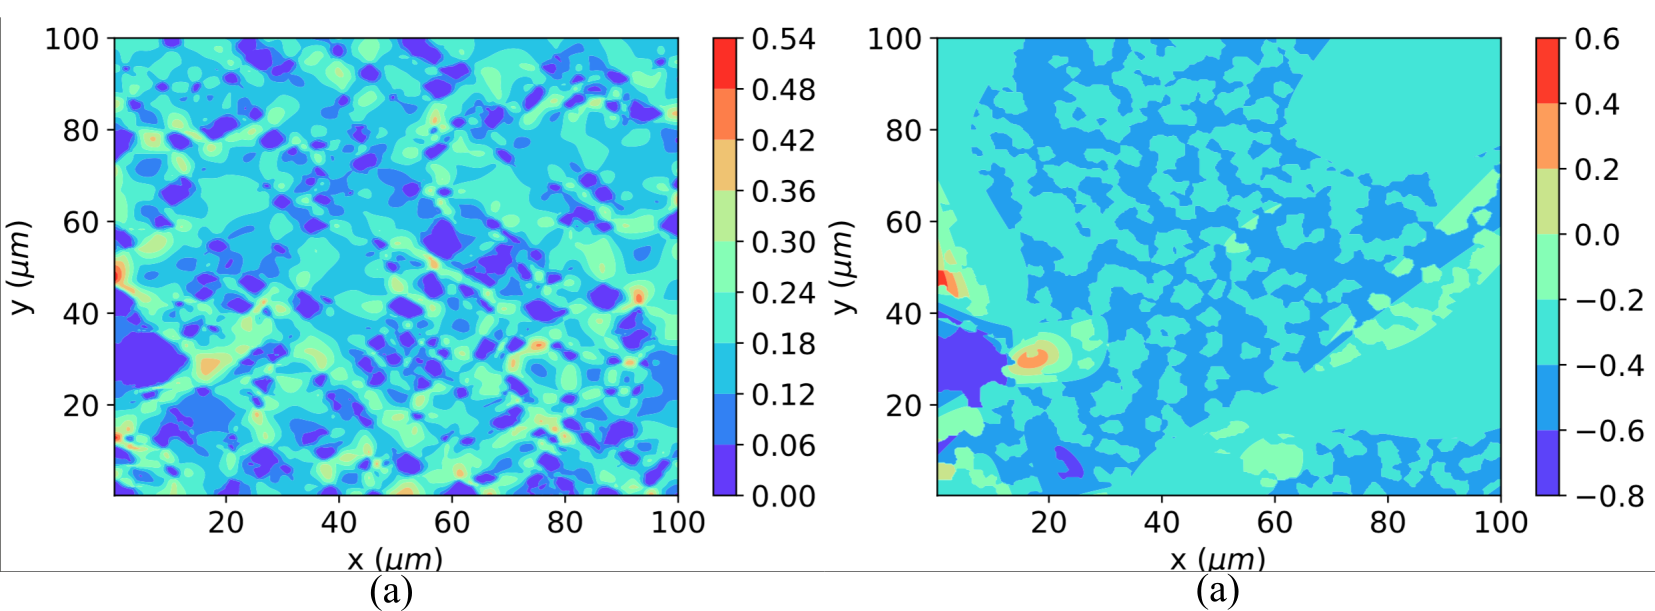
\includegraphics[width=0.95\textwidth]{Pictures/ann-res/ann-contours.png}
	\hspace{1mm}
	\caption{Effective Strain contour plots for (a) FE and (b) ANN predicted values.} 
	\label{fig:ann-contours}
\end{figure}
\newpage
\section{LSTM Model Results}
The LSTM Model shows significantly better performance than the ANN model. Plastic deformation being a history-dependent process, the output variable prediction is better modeled using LSTMs as they treat data as a time series. LSTMs maintain a context over time making them efficient in time series predictive modeling problems. Our model was able to achieve very high $R^2$ values for all the three output variables here, namely, effective strain (${\bar{\epsilon}}$), von Mises effective stress ($\bar{\sigma}$) and stress triaxiality ratio. The high accuracy of the model can be observed from the plots in
Figure \ref{fig:exp_pred_lstm}. Table \ref{tab:diff-lstm-table} shows results from LSTM models trained with different number of layers. Each layer contains 200 neurons and all the models take under 15 minutes to train. The training time here is 7 times less than our best ANN model. 

\begin{table}
\begin{center}
\begin{tabular}{|c|c|c|c|c|c|}
\hline
Layers & MSE & \multicolumn{3}{c|}{$R^2$} \\
\hline
 & & ${\bar{\epsilon}}$ & $\bar{\sigma}$ & tri \\
\hline
2 & $2.93 \times 10^{-6}$ & 0.89 & 0.99 & 0.51\\
4 & $2.78 \times 10^{-5}$ & 0.89 & 0.89 & 0.92\\
8 & $4.74 \times 10^{-5}$ & 0.90 & 0.96 & 0.97\\
16 & $0.02$ & -1.20 & 0.93 & 0.96\\
\hline
\end{tabular}
\end{center}
\caption{Study of accuracy of models with different depths. All layers have 200 neurons.}
\label{tab:diff-lstm-table}
\end{table}
\begin{figure}[!h]
	\centering
	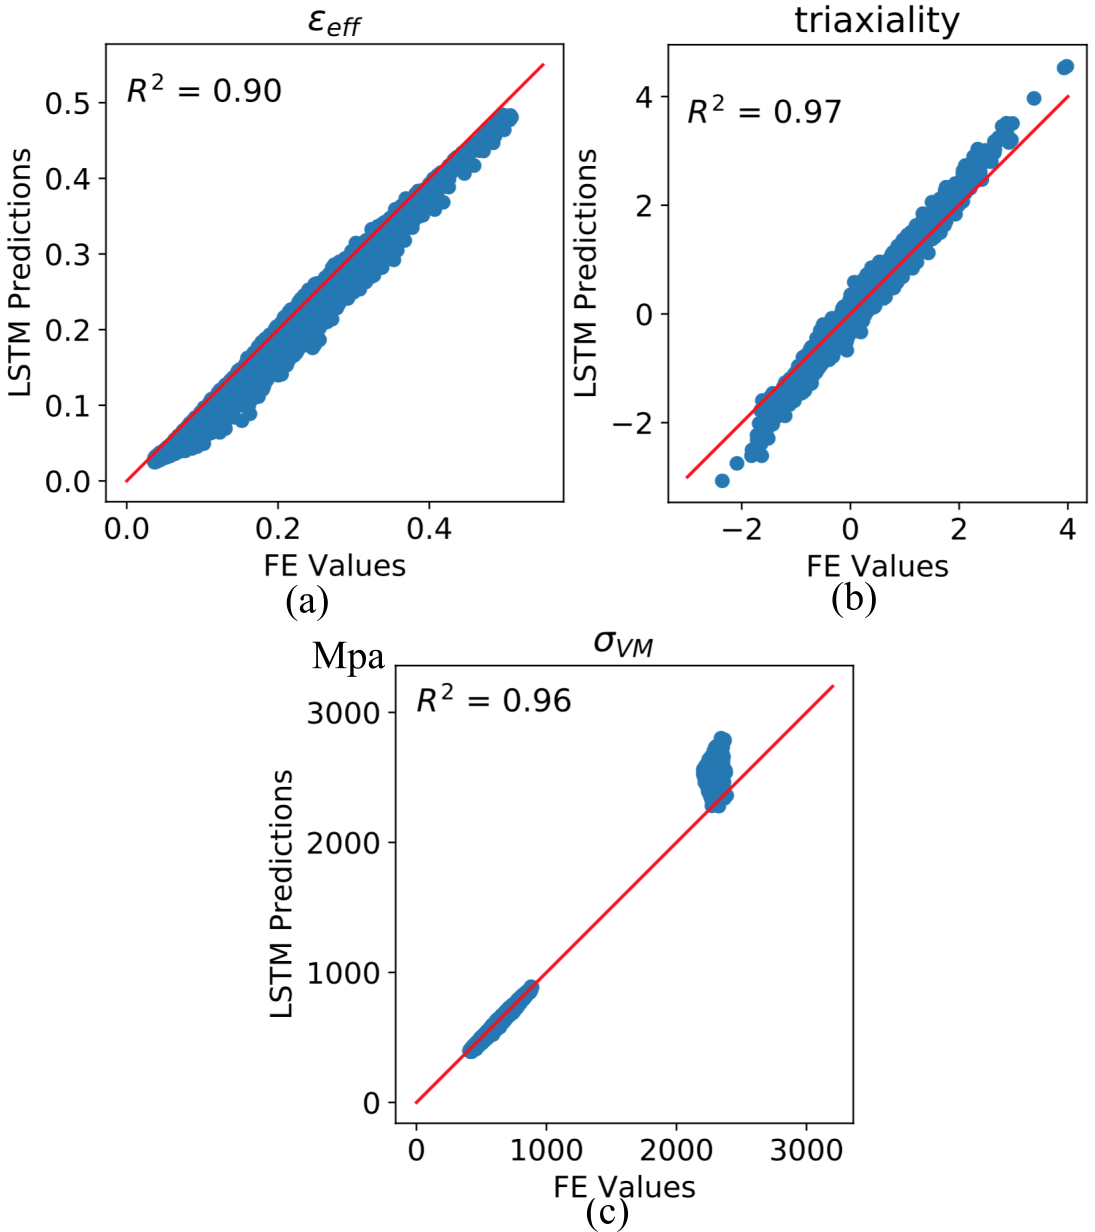
\includegraphics[width=0.8\textwidth]{Pictures/lstm-res/final-lstm-bitmap.png}
	\hspace{1mm}
	\caption{Plot of LSTM predicted values vs FE values for (a) effective strain, (b) triaxiality, (c) von Mises effective stress. Note that all the variables are normalized.} 
	\label{fig:exp_pred_lstm}
\end{figure}

Finally, figures \ref{fig:eff_strain_bitmap}, \ref{fig:tri_bitmap} and \ref{fig:vonmises_bitmap} show the contour plots for the different predicted variable at the last strain step. The contour plots depict how the model has successfully captured local behaviour of the microstructure. In figure-\ref{fig:vonmises_bitmap}, the predicted stress values higher than the FE values but the regions with high stress have been captured with good accuracy.
% \begin{figure}[hbtp]
% \begin{center}
% 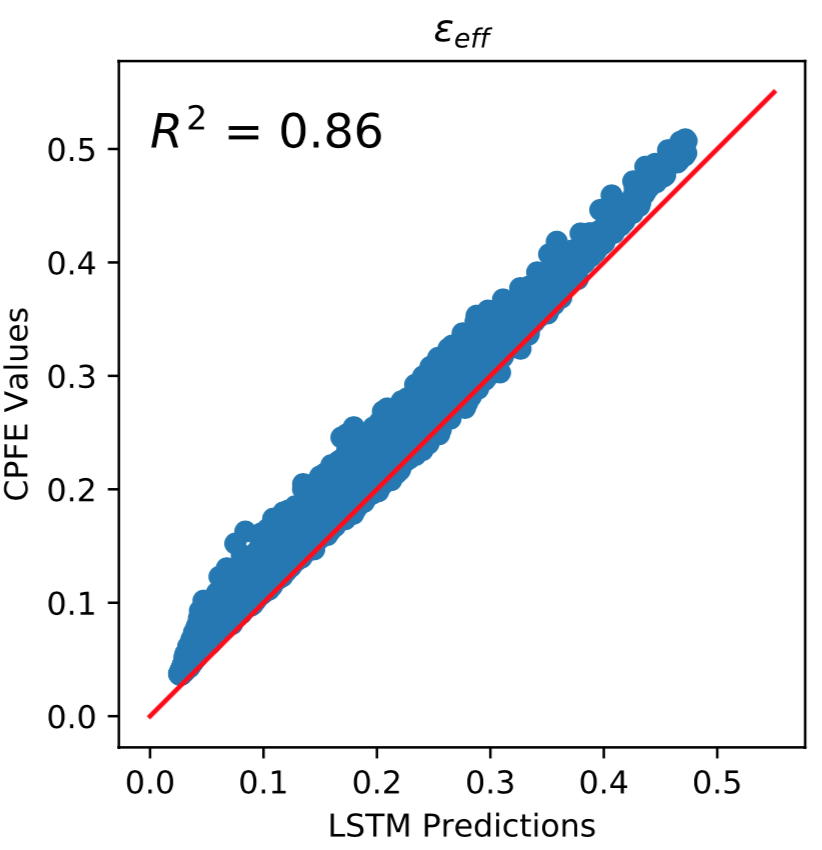
\includegraphics[scale=0.4]{Pictures/lstm-res/strain_eff.png}
% 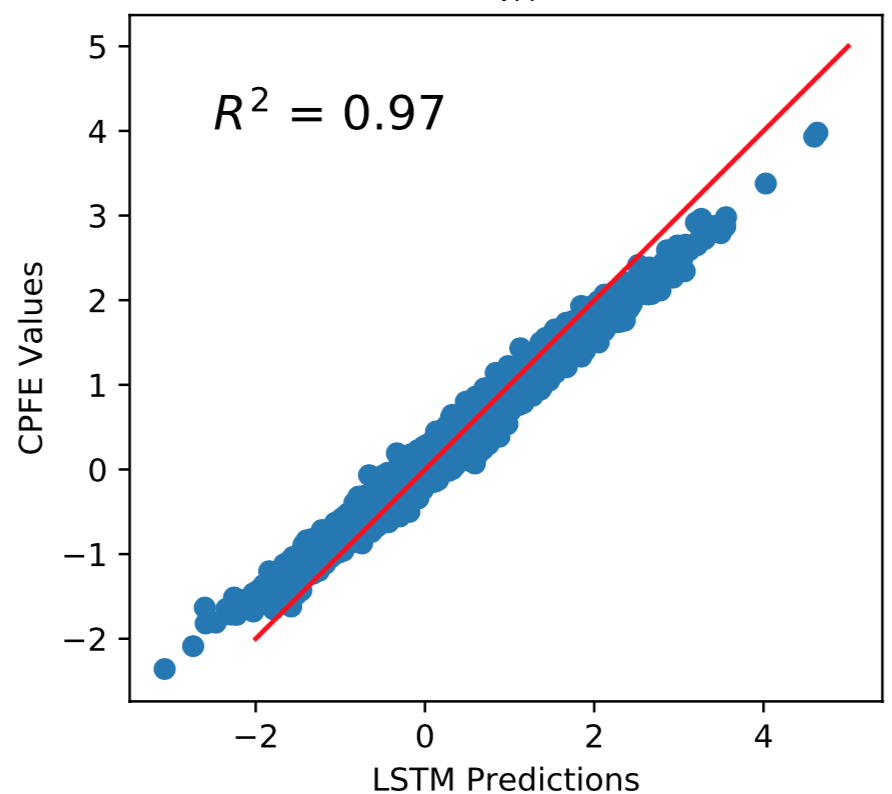
\includegraphics[scale=0.4]{Pictures/lstm-res/tri.png}
% \end{center}
% \begin{center}
% 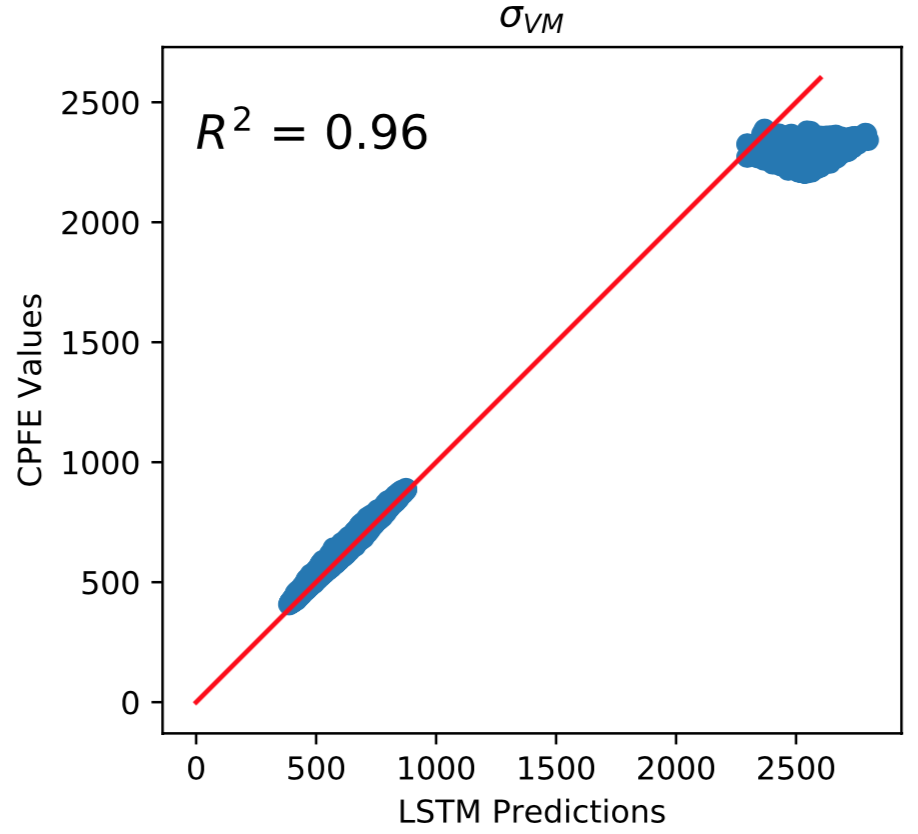
\includegraphics[scale=0.4]{Pictures/lstm-res/vonmises.png}
% \end{center}
% \caption{Plots of ANN Predictions vs CPFE Values for all the output variables}
% \label{fig:exp_pred_lstm}
% \end{figure}

\begin{figure}[!h]
	\centering
	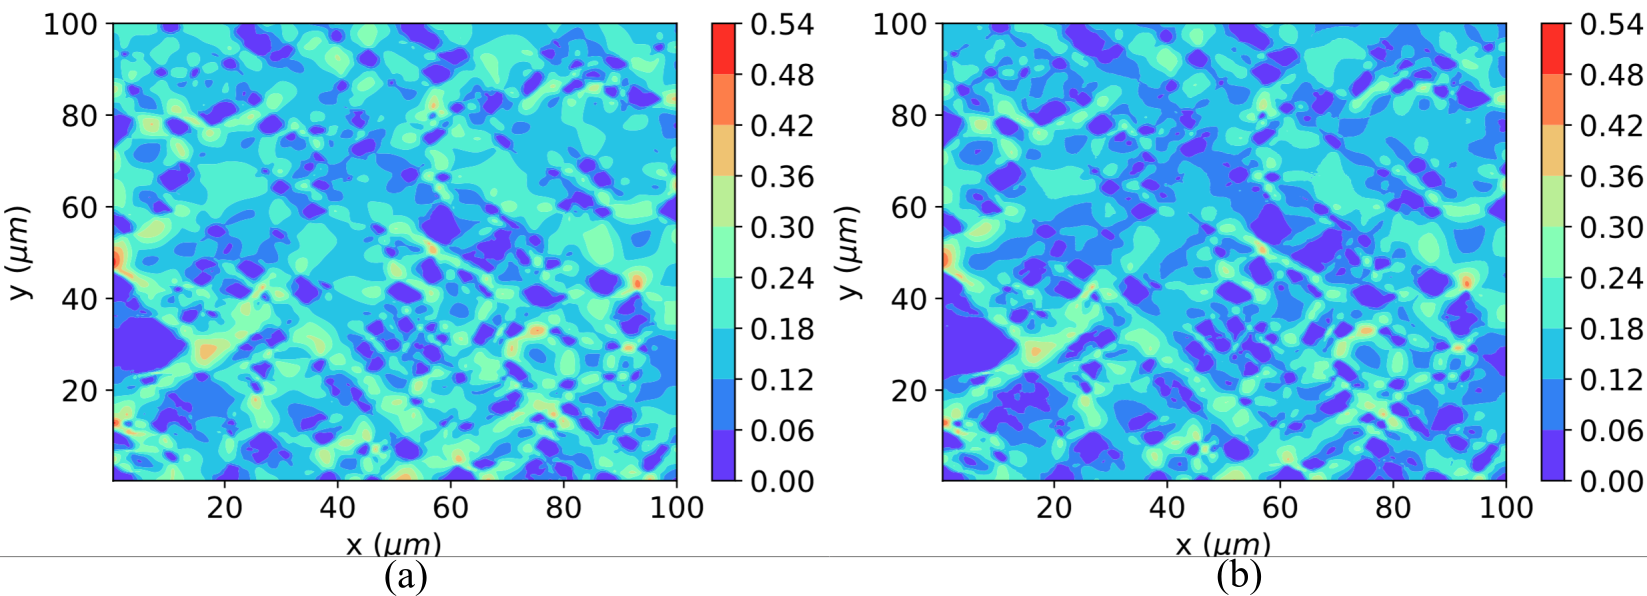
\includegraphics[width=0.95\textwidth]{Pictures/lstm-res/eff_strain_bitmap.png}
	\hspace{1mm}
	\caption{Effective Strain contour plots for (a) FE and (b) LSTM predicted values.} 
	\label{fig:eff_strain_bitmap}
\end{figure}

\begin{figure}[!h]
	\centering
	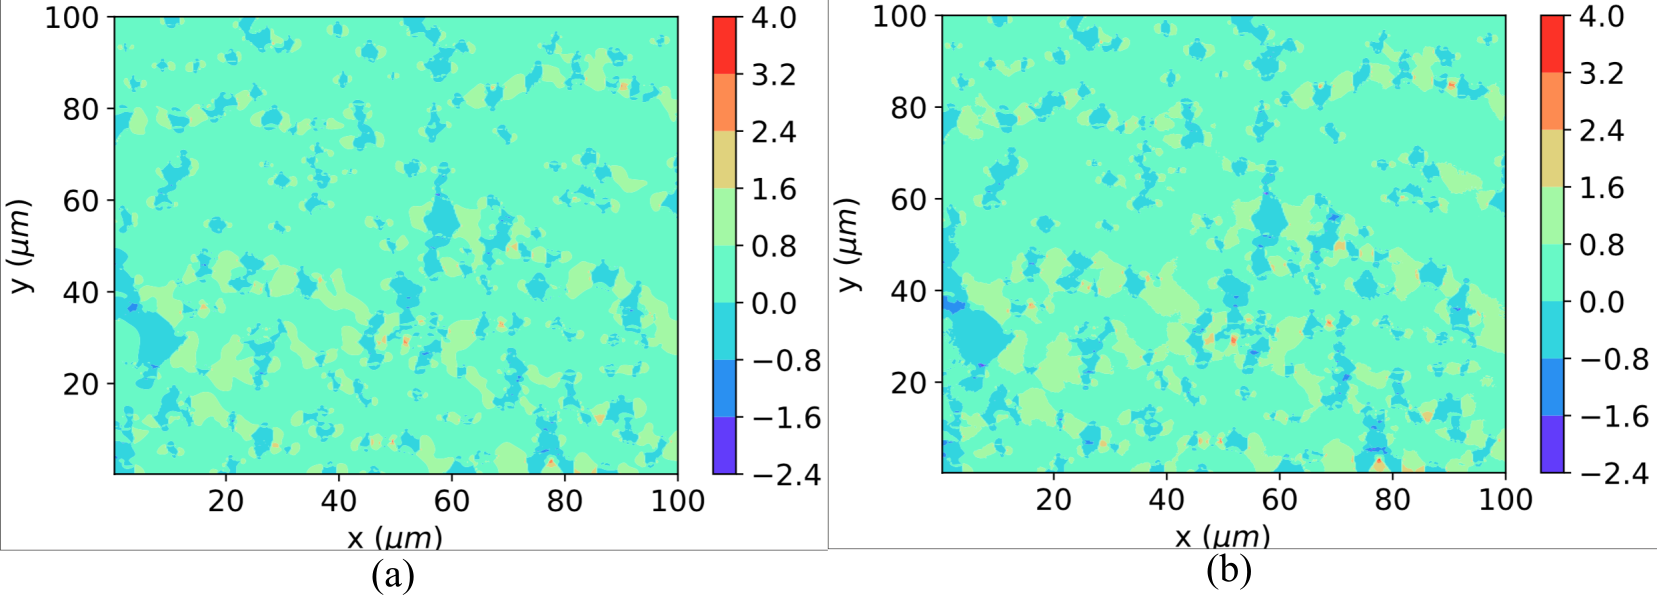
\includegraphics[width=0.95\textwidth]{Pictures/lstm-res/tri_bitmap.png}
	\hspace{1mm}
	\caption{Triaxiality contour plots for (a) FE and (b) LSTM predicted values.} 
	\label{fig:tri_bitmap}
\end{figure}

\begin{figure}[!h]
    \centering
	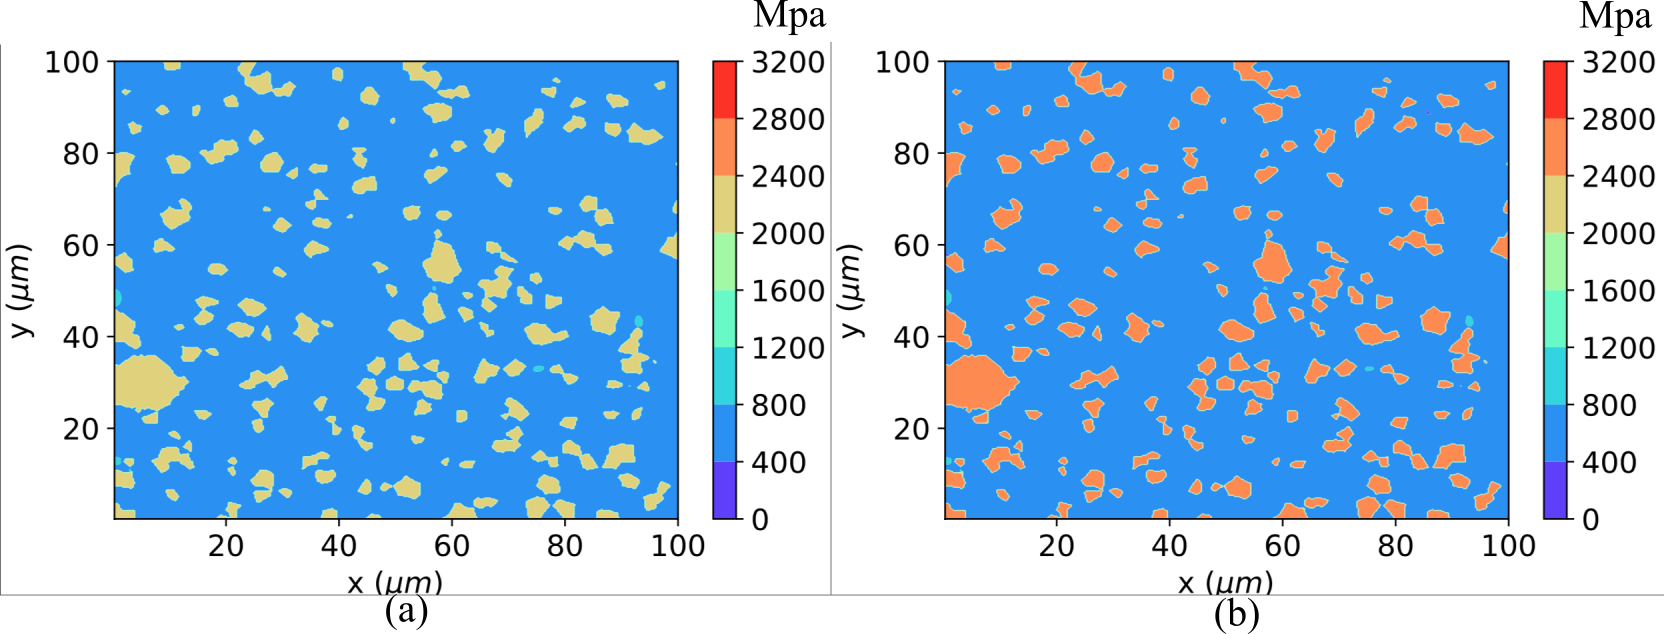
\includegraphics[width=0.95\textwidth]{Pictures/lstm-res/vonmises_bitmap-units.png}
	\hspace{1mm}
	\caption{Vonmises contour plots for (a) FE and (b) LSTM predicted values.} 
	\label{fig:vonmises_bitmap}
\end{figure}
% Chapter Template

\chapter{Conclusion} % Main chapter title

\label{Chapter5} % Change X to a consecutive number; for referencing this chapter elsewhere, use \ref{ChapterX}

\lhead{Chapter 5. \emph{Conclusion}} % Change X to a consecutive number; this is for the header on each page - perhaps a shortened title

%----------------------------------------------------------------------------------------
%	SECTION 1
%----------------------------------------------------------------------------------------

\section{Summary}

We have applied two machine learning models, namely, artificial neural networks (ANNs) and long short term memory (LSTM), a type of recurrent neural network (RNN) to predict the deformation of DP steel microstructures. J2 plasticity simulations are run for the 2D dual-phase ferrite-martensite microstructures. The results of these simulations are used as the ground truth for the machine learning model training. We start with employing an ANN to make predictions for effective strain, von Mises effective stress and triaxiality. After a systematic parametric study for the hyper parameters of the model, the accuracy of the ANN models was found to be very low. ANNs do not deal with temporal or spatial information. The higher errors may also be a result of discretizing our dataset into $0.01$ strain steps. 

As plasticity is a history-dependent process, RNNs are presumably a better option. LSTMs were applied to deal with the temporal nature of our data. The results obtained from LSTM model have an error value 3 order less than that of the ANN. The model makes predictions at $0.01$ strain intervals. Our method does not need to perform numerical iterations per strain step, otherwise needed by the conventional methods. The main strength of the LSTM model over ANN, is the reduction in computational time. The training time is 7 to 8 times less than that for ANN and predictions only take a few seconds. This ML-surrogate model trained and tested on simulated data is highly accurate and orders of magnitude faster than conventional micromechanical models. 

\section{Future Work}
The models developed has been trained and tested for microstructure with defined phase fractions and fixed boundary conditions. The framework can be extended to predict the evolution of series of other mircomechanical properties. Furthermore, more microstructures can be generated with various macroscopic conditions and microstructure evolution for a more general case can be predicted. 
%% Chapter Template

\chapter{Model Development} % Main chapter title

\label{Chapter3} % Change X to a consecutive number; for referencing this chapter elsewhere, use \ref{ChapterX}

\lhead{Chapter 3. \emph{Model Development}} % Change X to a consecutive number; this is for the header on each page - perhaps a shortened title

%----------------------------------------------------------------------------------------
%	SECTION 1
%----------------------------------------------------------------------------------------

\section{Finite Element Modeling Framework}
%-----------------------------------
%	SUBSECTION 1
%-----------------------------------
\subsection{Microstructure Instantiation}
We have used an in-house MATLAB code to instantiate the 2D microstructures of a dual-phase (DP) steel comprising of ferrite and martensite phases. This code employs a weighted Voronoi tessellation algorithm for random positioning of grain centers within the simulation domain. The grain size distribution and volume fractions of the respective phrases are pre-defined based on experimental measurements. Figure-\ref{fig:grain-trans} shows the grain map of the microstructure generated by this algorithm. The desired mean radius $r_i$ and  volume fractions $V_i$ are given as inputs to the algorithm. The number of grains are calculated by the algorithm as $(Area\times V_i)/(\pi r_i^2)$. The sizes of these $n_i$ grains are generated randomly. The subscript $i$ has a value of 1 for ferrite and 2 for martensite. Details of the microstructure instantiation algorithm are given in Ref.  \cite{patra2015modeling}. The Trelis meshing software has been used to mesh the 2D microstructure with voxel-based elements. An element size of $0.25 \mu m$ is used to mesh the simulation domain of $100\times100 \mu m^2$.
\begin{figure}[!h]
	\centering
	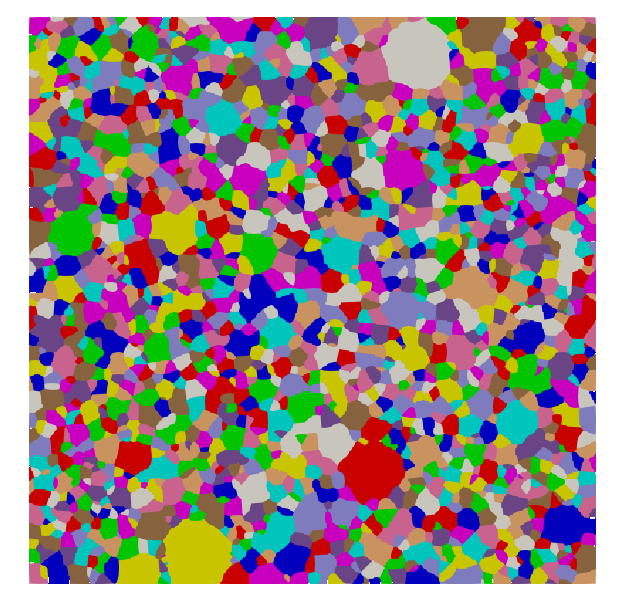
\includegraphics[width=0.65\textwidth]{Pictures/grain-trans.png}
	\hspace{1mm}
	\caption{Grain Map (colours are random and only to demarcate one grain from another)} 
	\label{fig:grain-trans}
\end{figure}
%-----------------------------------
%	SUBSECTION 2
%-----------------------------------
\subsection{Constitutive Model}
We have used a J2 plasticity constitutive modeling framework for the finite element (FE) computations. This framework is based on a finite deformation, dislocation density based model adapted from a crystal plasticity model previously used to model deformation behavior of various metallic systems \cite{POKHAREL2019201} \cite{THOOL2020102785}. While this is not a new feature of this work, details are provided here for completeness. 

In this framework, the deformation gradient is multiplicatively decomposed into the elastic and plastic parts: 
\begin{equation}
\boldsymbol{F} = \boldsymbol{F^e} \cdot \boldsymbol{F^p}
\end{equation}
where, $\boldsymbol{F^p}$ relates the reference configuration to an intermediate configuration and accounts for shear due to plastic deformation, while $\boldsymbol{F^e}$ relates the intermediate configuration to the current, deformed deformation and accounts for the rigid body rotation and elastic distortion. 
The elastic Green strain is given as:
\begin{equation}
\boldsymbol{E^e} = \frac{1}{2} (\boldsymbol{F^e}^T \cdot \boldsymbol{F^e} - \boldsymbol{I})
\end{equation}
Further, the second Piola-Kirchoff tensor is related to the elastic Green strain via the fourth rank elasticity tensor $\boldsymbol{C_o}$, i.e.,
\begin{equation}
    \boldsymbol{\sigma^{PK2}} = \boldsymbol{C_o} : \boldsymbol{E^e}
\end{equation}
The second Piola-Kirchoff tensor $\boldsymbol{\sigma^{PK2}}$ and the cauchy stress $\boldsymbol{\sigma}$
\begin{equation}
    \boldsymbol{\sigma} = \frac{\boldsymbol{F^e} \cdot \boldsymbol{\sigma^{PK2}} \cdot \left (\boldsymbol{F^e}\right)^T}{det\left (\boldsymbol{F^e}\right)}
\end{equation}
The von Mises effective stress, $\bar{\sigma}$ can be given in terms of the deviatoric part $\boldsymbol{S}$ of the Cauchy stress, i.e.,
\begin{equation}
    \boldsymbol{S} = dev(\boldsymbol(\sigma)) = \boldsymbol{\sigma} - \frac{\left (tr(\boldsymbol{\sigma}) \right )\boldsymbol{I}}{3}
\end{equation}
\begin{equation}
    \bar{\sigma} = \sqrt{\frac{3}{2}\boldsymbol{S}:\boldsymbol{S}}
\end{equation}
In J2 plasticity, the equivalent plastic strain rate $\dot{\bar{\epsilon}}^p$ is given as a function of the von Mises effective stress $\bar{\sigma}$. In this finite deformation framework, the plastic deformation gradient is related to the plastic velocity gradient as: $\boldsymbol{\dot{F}^p} = \boldsymbol{L^p} \cdot \boldsymbol{F^p}$, where $\boldsymbol{L^p}$ is the velocity gradient given by:
\begin{equation}
    \boldsymbol{L^p} = \dot{\bar{\epsilon}}^p \cdot \boldsymbol{N^p}
\end{equation}
where $\dot{\bar{\epsilon}}^p$ is the effective plastic strain, and $\boldsymbol{N^p}$ gives the direction of the plastic flow given by:
\begin{equation}
   \boldsymbol{N^p} =  \sqrt{\frac{3}{2}}\frac{\boldsymbol{S}}{\bar{\sigma}}
\end{equation}
The equivalent plastic strain rate is modelled using a Kocks-type activation enthalpy-driven flow rule:
\begin{equation}
\dot{\bar{\epsilon}}^p = \dot{\bar{\epsilon}}^p_o\exp\left(\frac{-\Delta F_g}{kT}\left(1 - \left(\frac{\sigma_{eff} - S_a}{S_t}\right)^p\right)^q\right)
\end{equation}
where, $\Delta F_g$ is the activation energy for dislocation glide, $S_a$ is athermal slip resistance, and $S_t$ is the thermal slip resistance, $p$ and $q$ are parameters used to model the shape of the activation enthalpy curve. The athermal slip resistance $S_a$ can be given by:
\begin{equation}
    S_a = \frac{h_p}{\sqrt{d}} + Gb\sqrt{q_p\rho}
\end{equation}
where, $h_p$ is the Hall-Petch hardening constant, $d$ is the grain size, $G$ is the shear modulus, $b$ is the Burgers vector, $q_p$ is the dislocation barrier strength and $\rho$ is the total dislocation density. $\rho$ is defined as the sum of immobile ($\rho_M)$ and mobile ($\rho_I)$ dislocation densities, i.e., 
\begin{equation}
    \rho = \rho_M + \rho_I
\end{equation}
The evolution of the dislocation densities with respect to time depends on the equivalent tensile plastic strain rate as:
\begin{equation}
\dot{\rho_M} = \frac{k_mul}{b}\sqrt{\Sigma\rho}|\dot{\bar{\epsilon}}^p| - \frac{2R_c}{b}\rho_M|\dot{\bar{\epsilon}}^p| - \frac{1}{b\lambda}|\dot{\bar{\epsilon}}^p|
\end{equation}
\begin{equation}
\dot{\rho_I} = \frac{1}{b\lambda}|\dot{\bar{\epsilon}}^p| - k_{dyn}\rho_I|\dot{\bar{\epsilon}}^p|
\end{equation}
where $\lambda = \frac{1}{\beta\sqrt{\rho}}$ is effective mean free path, $\beta$ is a constant associated with dislocation trapping, $k_{mul}$ is the dislocation multiplication rate constant and $R_c$ is the critical capture radius. The first term in Eq. 3.12 represents the multiplication of mobile dislocations at existing dislocations, while the second term represents the mutual annihilation of dislocation dipoles, and third term is the trapping of mobile dislocations at barriers. $k_{dyn}$ is the material constant associated with dynamic recovery of immobile dislocations due to thermally activated processes. The first term in Eq. 3.13 represents the rate at which mobile dislocations are trapped in barriers and become immobile, while the second term is the rate at which the immobile dislocations are annihilated due to dynamic recovery.

The constitutive model has been implemented as material model and interfaced with the open source finite element code, MOOSE \cite{permann2020moose}. The individual phases have been calibrated to the response of the ferrite and martensite phases based on available data in the literature. Further details and model parameters are given in Basu et al \cite{soudip}.

\subsection{Loading And Boundary Conditions}
A mesh size of $0.25 \mu m$ is used with a simulation domain size of $100\times100 \mu m^2$. The simulation domain has 40,000 elements.A generalized plane strain assumption is used in these essentially 2D simulations. The bottom face of the simulation domain is constrained in the y-direction, while the left face is constrained in the x-direction to resemble an axisymmetric model. The corner node common to both these faces is fully constrained to prevent rigid body motion. Displacement-controlled tensile loading is applied on the top face at a strain rate of $5\times10^{-3}s^{-1}$.
\begin{figure}[!h]
	\centering
	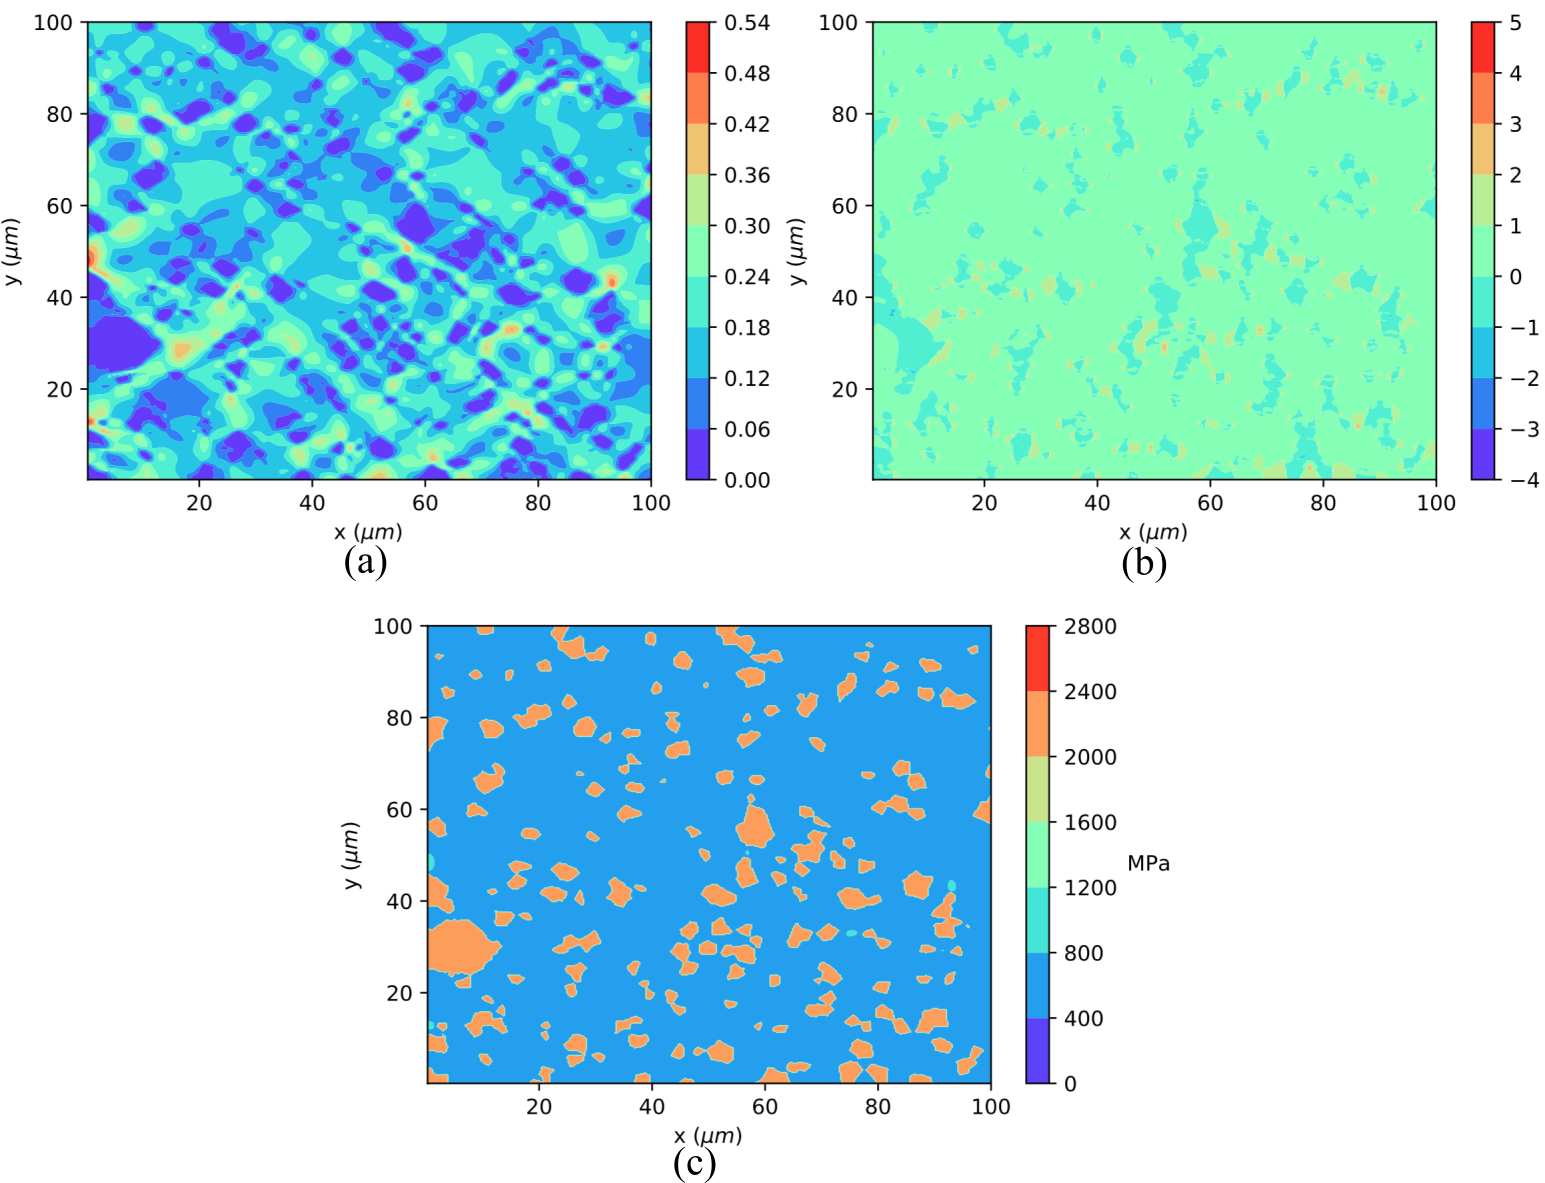
\includegraphics[width=\textwidth]{Pictures/result-fe.png}
	\hspace{1mm}
	\caption{Contour of (a) Effective Strain (b) Triaxiality (c) Vonmises Stress at the last time step} 
	\label{fig:exo-plots}
\end{figure}
\begin{figure}[!h]
	\centering
	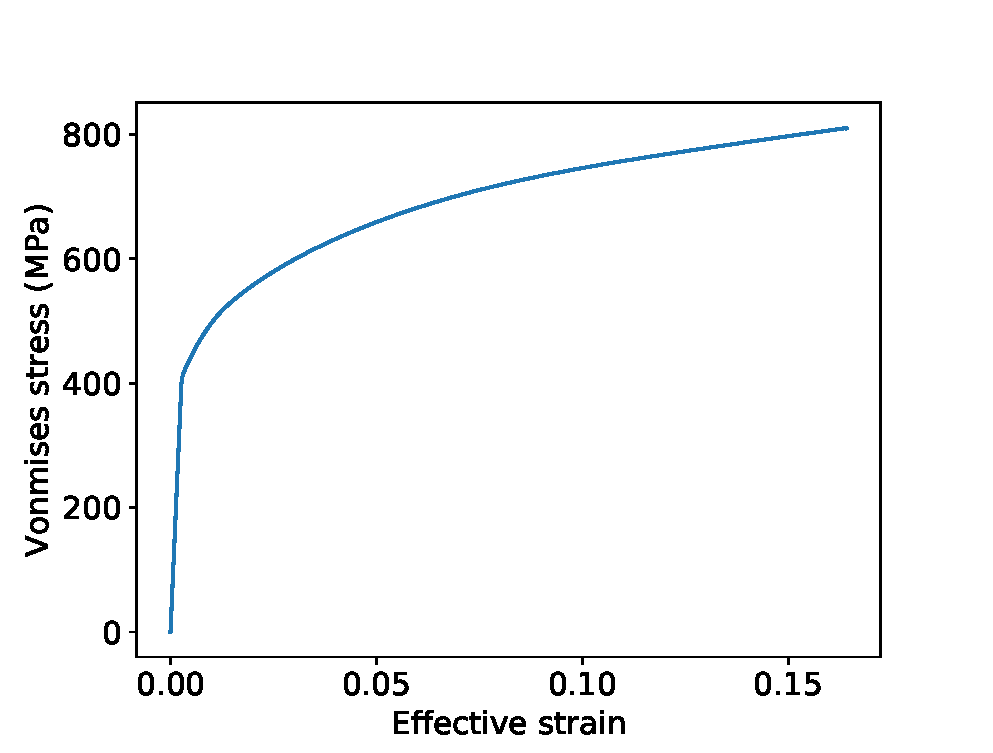
\includegraphics[width=0.8\textwidth]{Pictures/stress-strain.eps}
	\hspace{1mm}
	\caption{Effective strain vs Vonmises stress curve} 
	\label{fig:stress-strain}
\end{figure}

\section{Data Extraction from FE Results}
The simulation results of the FE model are output to an EXODUS data file. The EXODUS format is a binary file which is used for FE pre- and post-processing. Data used to define the finite element mesh, along with both the boundary conditions and load application points are includes in the file. The EXODUS format is advantageous as it combines the mesh data as well as the results data in a single file. This assures the user that the results are consistent with the model \cite{mills1988exodus}. However, to access this data in a usable and easily interpretable way, special software are used. For the purpose of this project, we have used the  Sandia Engineering Analysis Code Access System (SEACAS) developed by Sjaardema \cite{seacas}. The library consists of packages which can convert an EXODUS file's data to different formats like text file and MATLAB data files. The Python package has been used for this project which makes reading the data from an EXODUS file viable through a python script. The package provides a number of predefined functions to extract different information from the EXODUS file. Using these functions, we have extracted all the data from the EXODUS file to a csv format. The csv format has all the element variable values at every time-step for every element. The script is written in Python 2.7.17 and take approximately 10 minutes to execute. The time taken by the script varies with the mesh size and number of variables in the exodus file.   

\section{Machine Learning Framework}
\subsection{ANN Model}
At the basic level, the process of developing an ANN model (or any learning model) has two primary steps. First one being, selecting the relevant, representative and compact set of  features and then developing a relation between them to get the desired result. Elimination of irrelevant features and selection or relevant ones is one of the central tasks in machine learning \cite{blum1997selection}. In this context, it has been assumed that the observed heterogeneity in deformation is due to the underlying heterogeneity of the microstructure. The features of interest are highlighted in the Table \ref{tab:feature-table}. 
\begin{table}
\begin{center}
\begin{tabular}{|c|c|}
\hline
Feature & Description \\
\hline
\textit{x} & x-coordinate of the element \\
\hline
\textit{y} & y-coordinate of the element \\
\hline
\textit{p} & Phase to which the element belongs (ferrite or martensite) \\
\hline
\begin{math}{\epsilon_{app}}\end{math}& Applied (or nominal) strain \\
\hline
\end{tabular}
\end{center}
\caption{\label{tab:feature-table}Selected feature names and descriptions.}
\end{table}

The output variables of interest are effective strain, ${\bar{\epsilon}}$, von Mises effective stress, $\bar{\sigma}$, and stress triaxiality ratio. While, effective strain and effective stress can be correlated with plastic deformation in the respective phases, the stress triaxiality ratio (given as the ratio of the mean stress over the von Mises effective stress) provides a measure of the development of multi-axial stress states that may contribute to eventual failure initiation in the material. In the present context, the ferrite-martensite interfaces are potential sites for failure initiation in DP steels and hence it is pertinent to be able to predict the stress triaxiality ratio as well. For each element, ${\bar{\epsilon}}$, $\bar{\sigma}$ and triaxiality ratio are recorded at applied strain intervals of $0.01$. The simulation is run up to $0.15$ nominal strain, thus providing us a total of fifteen datasets at $0.01$ nominal strain intervals. The mesh consists of $400\times400$ elements, making the length of every feature and target variable vector $2,400,000$. Thus, the shape of our input is $2,400,000\times4$ and the corresponding shape of output is $2,400,000\times3$. 

Note that feature selection depends on the output variables of interest and may vary if it is desired to output a different set of variables. Mangal and Holm \cite{MANGAL2018122} provide a detailed study of the performance of neural network models with different input features for a crystal plasticity model. In the context of a J2 plasticity model, we assume the features given in Table \ref{tab:feature-table} to be the most relevant for the present problem.

Any ANN model is very sensitive to the magnitude of the training data. Given that we are interested in strains and stresses, whose magnitudes are generally many orders apart, all the data has been normalized within the range $[0,1]$ in the present work. The normalised values $x_i^n$ for any training variable $x_i$ are calculated as:
\begin{equation}
    x_i^n = \frac{x_i - x_{min}}{x_{max} - x_{min}}
\end{equation}
In this work, the mean-squared error function (MSE) has been used and the sigmoid function has been employed as the activation function for every neuron. The completed training and model development process has been performed using python and Keras with a Tensorflow backend. Data splitting is another important task during data splitting where hold-out validation is employed to ensure generalisation \cite{may2010data}. The dataset is split into training ($80\%$) and testing ($20\%$) datasets. The training data is used to for training and learning of the ANN, whereas the testing dataset is used to check the accuracy of the fitted parameters. The validation dataset is unseen by the ANN model, therefore predictions made by the model on the validation dataset represents the degree to which the model generalizes over our data. A number of networks were trained on this data with different architectures. The network which performed relatively better than others consisted of 4 inputs, 3 hidden layers and 3 outputs. The training of the neural network is performed over 5 epochs and takes 106 minutes to train. 
\begin{figure}[!h]
	\centering
	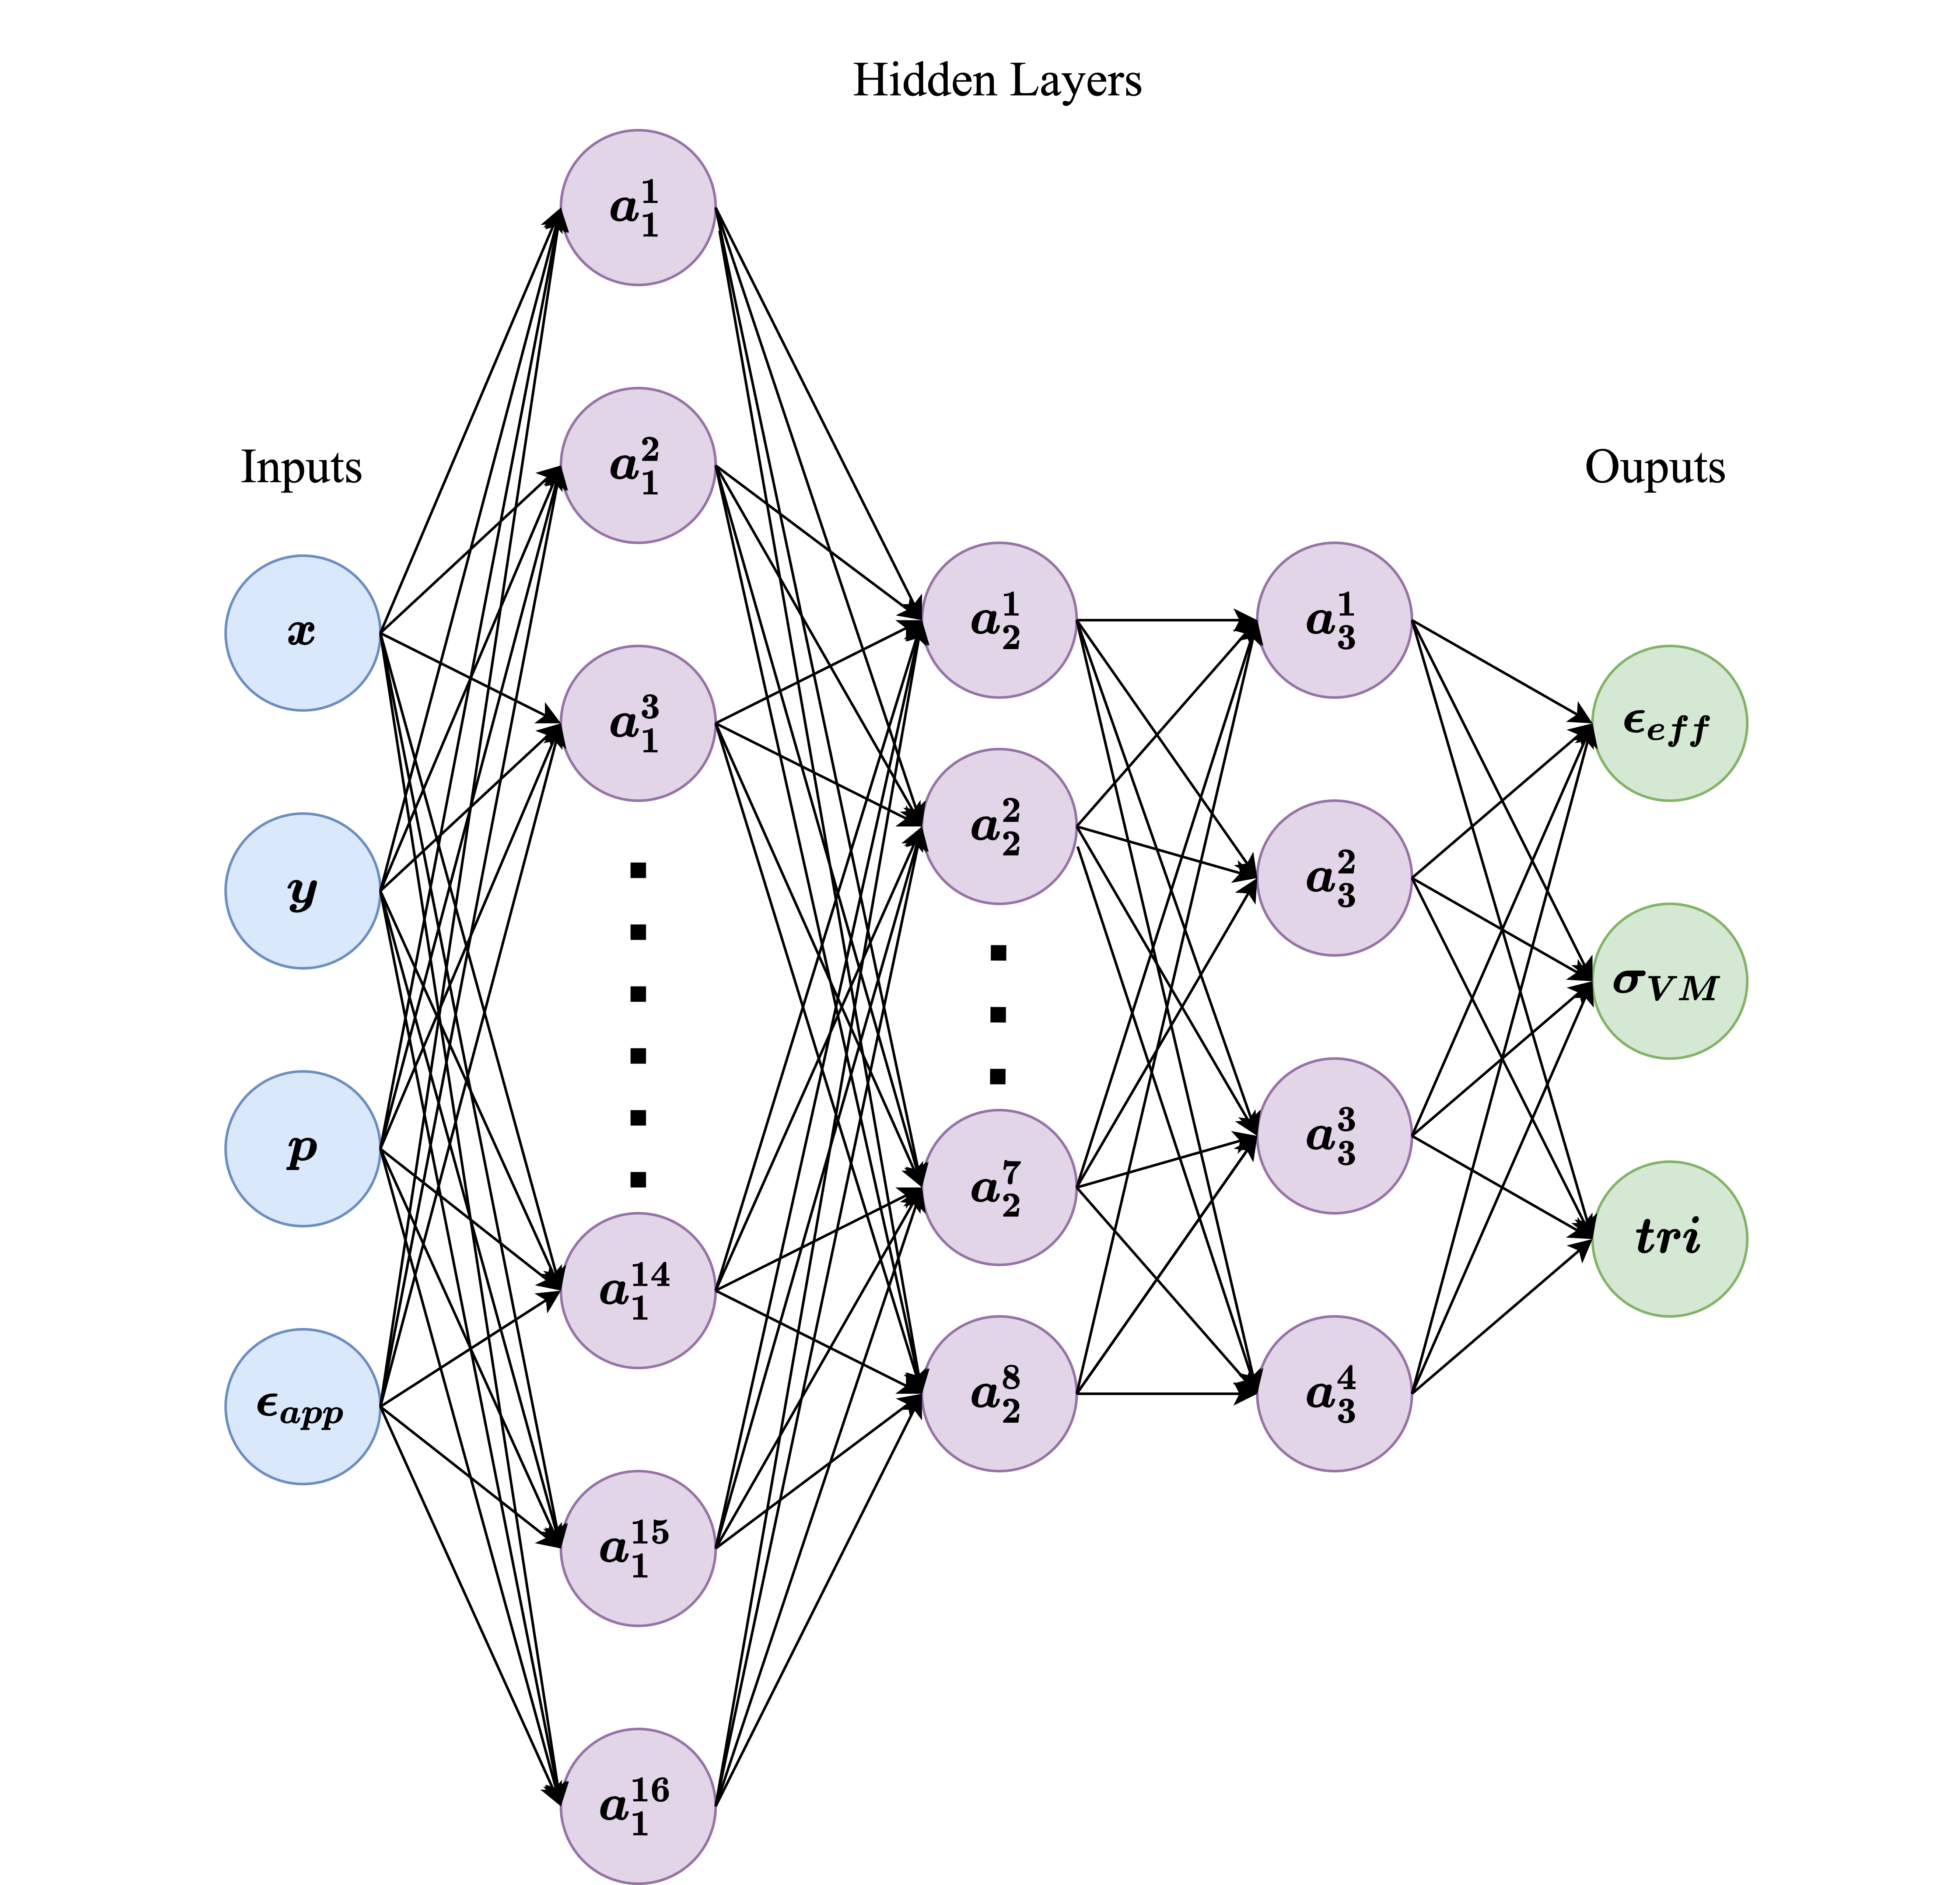
\includegraphics[width=0.9\textwidth]{Pictures/my-ann.png}
	\hspace{1mm}
	\caption{Schematic of proposed ANN architecture} 
	\label{fig:my-ann}
\end{figure}
\begin{figure}[!h]
	\centering
	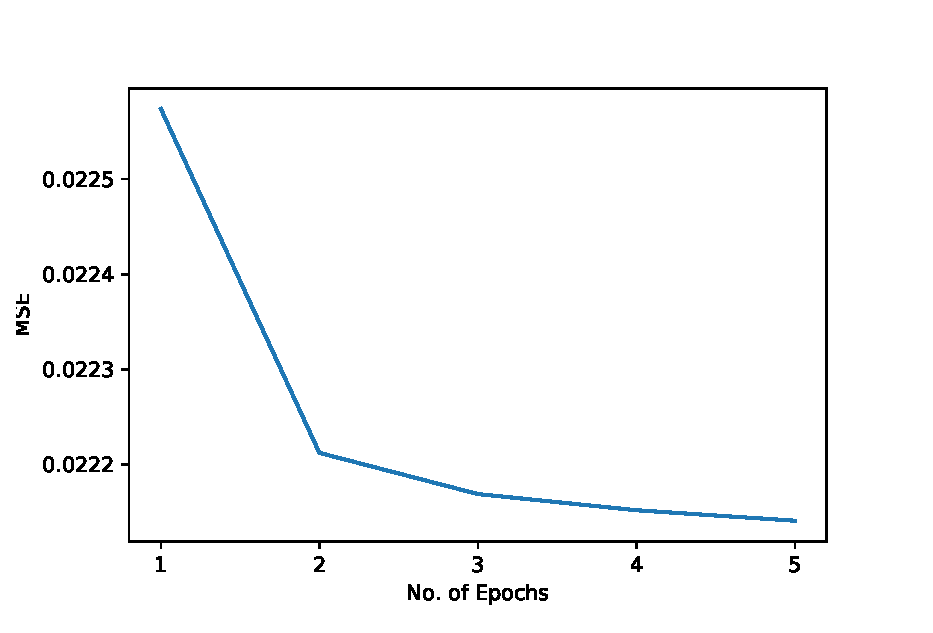
\includegraphics[width=0.8\textwidth]{Pictures/training_process.eps}
	\hspace{1mm}
	\caption{Learning curve showing the evolution of MSE loss over training data-set} 
	\label{fig:ann-training}
\end{figure}

\subsection{LSTM Model}
LSTMs have shown great accuracy in predicting sequence and time series data. The evolution of local strain distribution can be formulated as a sequence modeling problem. As with ANN, we are focusing on three output variables in our model, namely, effective strain, ${\bar{\epsilon}}$, von Mises effective stress,  $\bar{\sigma}$, and stress triaxiality ratio. For every element, the values of these variables are recorded for every $0.01$ nominal strain interval. As mentioned previously, the simulation is run till $0.15$ nominal strain and hence our data contains $15$ strain steps. Each element is associated with 3 sequences of length 15, and as there are $400\times400$ elements the total number of series or model predicts is $400\times400\times3$. For a given strain step $t$, $400\times400\times3$ length vector $\boldsymbol{X_t}$ is input to the LSTM model and used to predict the output vector, $\boldsymbol{Y_t}$ which consists of values at the next strain step in the series $X_{t+1}$. The structure of the data can be understood better through the Table \ref{tab:lstm-data-table}. All data was normalized within the range of $[0,1]$. The data was split into training ($70\%$) and test ($30\%$) datasets, meaning the training dataset consisted of only the first $10$ strain steps. The model was trained using the training dataset run over 300 epochs. The last $5$ strain steps were used to check how well the model performs on data it has not seen before. The model consists of $8$ LSTM layers with $200$ neurons in each layer. The activation function employed in this case is ReLU. The choice of activation function is driven by the reduction in MSE over the epochs. Figure \ref{fig:diff-activation-lstm} shows the performance of different activation functions while training the same dataset. The number of layers and neuron are the same for these model, only the variation with activation function is checked for. It can be observed that ReLU performs better than the other two activation functions by at least two orders of magnitude of MSE.

\begin{table}
\begin{center}
\begin{tabular}{|c|c|}
\hline
Input (\begin{math}\boldsymbol{X}\end{math})&Output (\begin{math}\boldsymbol{Y}\end{math}) \\
\hline
\begin{math}\boldsymbol{X_1}\end{math}& \begin{math}\boldsymbol{X_2}\end{math} \\
\begin{math}\boldsymbol{X_2}\end{math}& \begin{math}\boldsymbol{X_3}\end{math}  \\
\begin{math}\boldsymbol{X_3}\end{math}& \begin{math}\boldsymbol{X_4}\end{math} \\
. & . \\
. & . \\
. & . \\
. & . \\
\begin{math}\boldsymbol{X_{10}}\end{math}& \begin{math}\boldsymbol{X_{11}}\end{math} \\
\hline
\end{tabular}
\end{center}
\caption{\label{tab:lstm-data-table}Training data format for LSTM.}
\end{table}

\begin{figure}[!h]
	\centering
	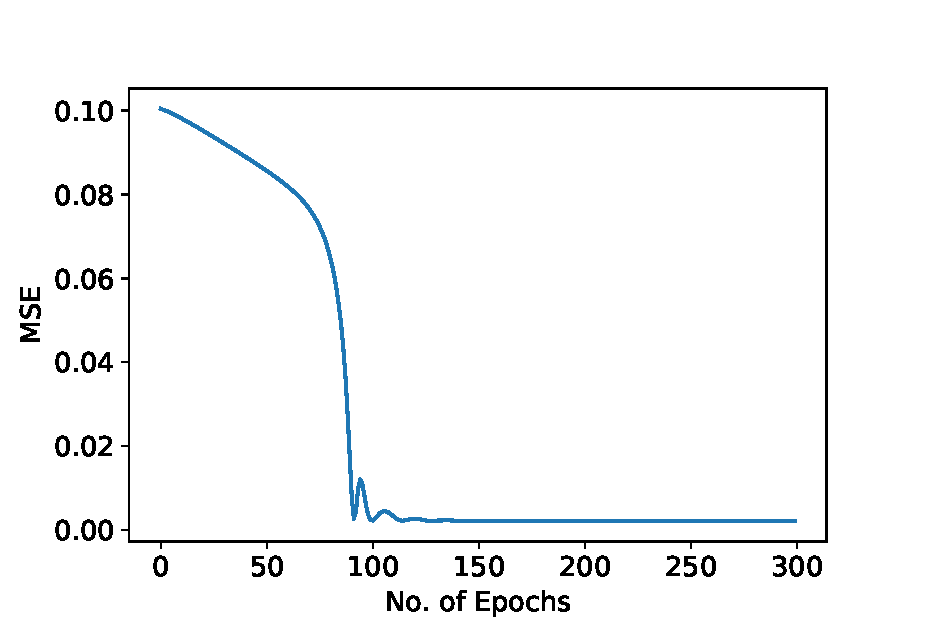
\includegraphics[width=0.7\textwidth]{Pictures/lstm-res/lstm-tanh_loss.eps}
	\hspace{1mm}
	\caption{Learning curve showing the evolution of MSE loss over training data-set.} 
	\label{fig:ann-training}
\end{figure}

\begin{figure}[!h]
	\centering
	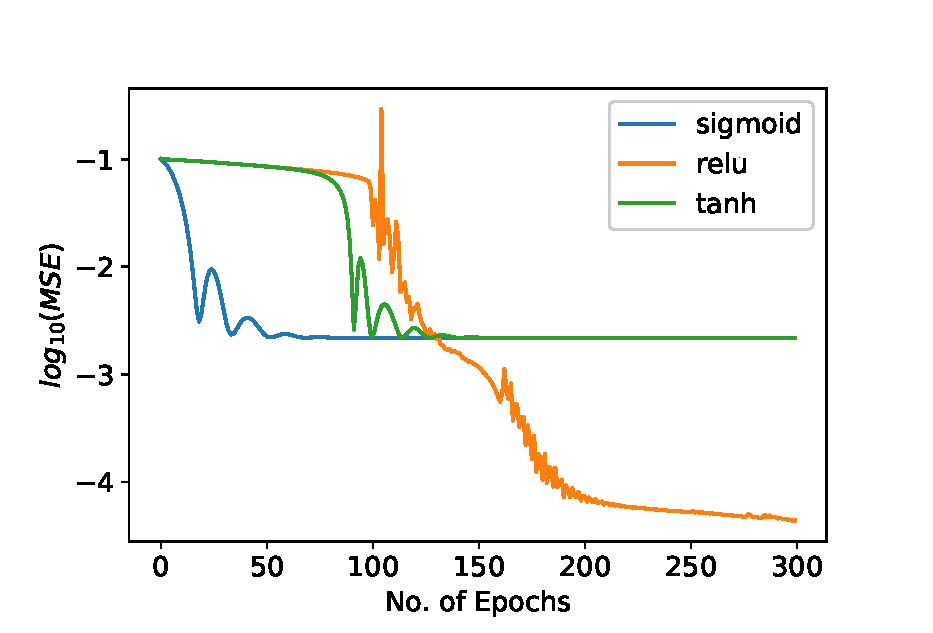
\includegraphics[width=0.7\textwidth]{Pictures/lstm-res/lstm-sctivations_log.eps}
	\hspace{1mm}
	\caption{Comparative study of MSE obtained in training models with different activation functions} 
	\label{fig:diff-activation-lstm}
\end{figure}
\begin{sidewaysfigure}[ht]
	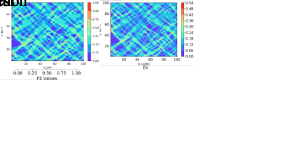
\includegraphics[width=0.95\textwidth]{Pictures/lstm-res/flow-purple.png}
	\hspace{1mm}
	\caption{Schematic representation of the proposed ML framework} 
	\label{fig:flow-chart}
\end{sidewaysfigure}
\iffalse
Along with a vanilla LSTM, two modification of LSTMs were also trained:
\begin{enumerate}
\item \textbf{Auto-regressive}: The training of procedure of this LSTM is similar to that of a vanilla LSTM, however the difference arises in the way predictions are made. For a regular LSTM, to predict the value of a sequence at time $t$ one would need to know all the true values till time $t-1$ and so on for $t+1$. In an auto-regressive methodology once an initial prediction is made using the available sequence data, all further predictions are made using this initial prediction. Say for example, a prediction is made for time $t$. To predict $t+1$ time-step, instead of using the input sequence data we use this predicted value at time $t$. This enables our LSTM to predict sequence values further into the future without requiring input data up to the penultimate step.
\item \textbf{LSTM-FC}: This kind of model consists two major components: (1) A long-short term memory based temporal simulator to model the local strain developments and (2) A neural network to capture the spatial dependencies of strain between a central element and it's neighbours. The LSTM capable of handling long term dependencies handles only the temporal information in the data, and the spatial information is incorporated using a fully connected neural network. The neural network is trained such that given 8 neighbouring elements' property values it can make predictions  for the central element. 
\end{enumerate}
\fi
%% Chapter Template

\chapter{Results and Discussion} % Main chapter title

\label{Chapter4} % Change X to a consecutive number; for referencing this chapter elsewhere, use \ref{ChapterX}

\lhead{Chapter 4. \emph{Results and Discussion}} % Change X to a consecutive number; this is for the header on each page - perhaps a shortened title

%----------------------------------------------------------------------------------------
%	SECTION 1
%----------------------------------------------------------------------------------------

\section{Artificial Neural Network (ANN) Results}
The relationship between the microstructure and mechanical behaviour of DP steels is extremely complex. Successful implementation of an ANN model would have helped understand these complex relations and helped in predicting experimental behavior of other heterogeneous systems. For assessing our model's predictive capabilities over three different variables simultaneously, a metric is used to estimate how well the model performs for each of these variables. For this purpose, we calculate the coefficient of determination, $R^2$. $R^2$ represents the proportion of variance that has been explained by the independent variables in the model. It provides an indication of goodness of fit and therefore a measure of how well unseen samples are likely to be predicted by the model, through the proportion of explained variance. Best possible score is 1.0 and it can be negative (because the model can be arbitrarily worse). This metric is given by the following equation:
\begin{equation}
    R^2(y, \hat{y}) = 1 - \frac{\sum_{i=1}^{n} (y_i - \hat{y}_i)^2}{\sum_{i=1}^{n} (y_i - \bar{y})^2}
\end{equation}
where $y$ is the actual output (true value) and $\hat{y}$ is the prediction made by the ANN model. For a model with $100\%$ accuracy then $y_i = \hat{y}_i)$ for all $i's$ making $R^2 = 1$, which indeed is the best case scenario. 

A number of neural network architectures were trained and their $R^2$ and mean squared error values were recorded for a comparative parametric study. The following table shows the results that were obtained along with the time taken to train each model. 

\begin{table}
\begin{center}
\begin{tabular}{|c|c|c|c|c|c|c|}
\hline
Layers & Architecture & MSE & Time & \multicolumn{3}{c|}{$R^2$} \\
\hline
&(Neurons in every layer) & & (hrs)& ${\bar{\epsilon}}$ & $\bar{\sigma}$ & tri \\
\hline
2 & 8,4 & 0.0221 & 1.44 & 0.55 & 0.16 & 0.7 \\
3 & 16,8,4, & 0.0221 & 1.76 & 0.55 & 0.16 & 0.07 \\
4 & 32,16,8,4 & 0.0221 & 1.78 & 0.55 & 0.17 & 0.06 \\
5 & 64,32,16,8,4 & 0.0222 & 1.82 & 0.55 & 0.15 & 0.05 \\
6 & 128, 64,32,16,8,4 & 0.0266 & 1.87 & 0.16 & 0.13 & 0.02 \\
7 & 256,128,64,32,16,8,4 & 0.0290 & 3.47 & $<0$ & $<0$ & $<0$ \\
8 & 512,256,128,64,32,16,8,4 & 0.0290 & 4.59 & $<0$ & $<0$ & $<0$ \\
9 & 1024,512,256,128,64,32,16,8,4 & 0.0289 & 7.32 & $<0$ & $<0$ & $<0$ \\
11 & 1024,1024,512,512,256,128,64,32,16,8,4 & 0.0290 & 20.24 & $<0$ & $<0$ & $<0$ \\
\hline
\end{tabular}
\end{center}
\caption{\label{tab:diff-ann-table}Study of accuracy of models with different depths and neurons.}
\end{table}

As can be clearly seen from the table, the model is unable to make the predictions successfully. The MSE is very high and the $R^2$ values too low. For the model to be acceptable, the MSE values should have been in the range of $10^{-4} - 10^{-5}$ and $R^2$ values should be above $0.80$. All the above simulations have run for 5 epochs. Increasing the epochs is usually accompanied by a decrease in error. However, even after increasing to 20 epochs, the $R^2$ values did not improve. The first architecture in Table \ref{tab:diff-ann-table} was trained for 20 epochs. The MSE reduced to 0.0216, but $R^2$ values remained approximately the same. Increasing the epochs increased the training time to 8.5 hours without yielding any significant results.  Increasing the dept and complexity of the network is another way to increase the accuracy. However, as can be seen from the table, the MSE and $R^2$ values actually worsen as the number of hidden layers are increased beyond 4. Another major drawback in the ANN model is the limited dataset we are using to train it. The data consists of only discrete data at $0.01$ strain intervals. If instead, we trained our data to smaller strain intervals of the FE simulations, the results would be perhaps better, albeit at the cost of significant training times.

ANN predicted values are plotted in Figure \ref{fig:exp_pred_ann} against the ground truth values to better visualize the performance of our model. Note that all results are plotted on the normalized scales. For an ideal case, all the data points would lie as close to the $y=x$ line.
\begin{figure}[!h]
	\centering
	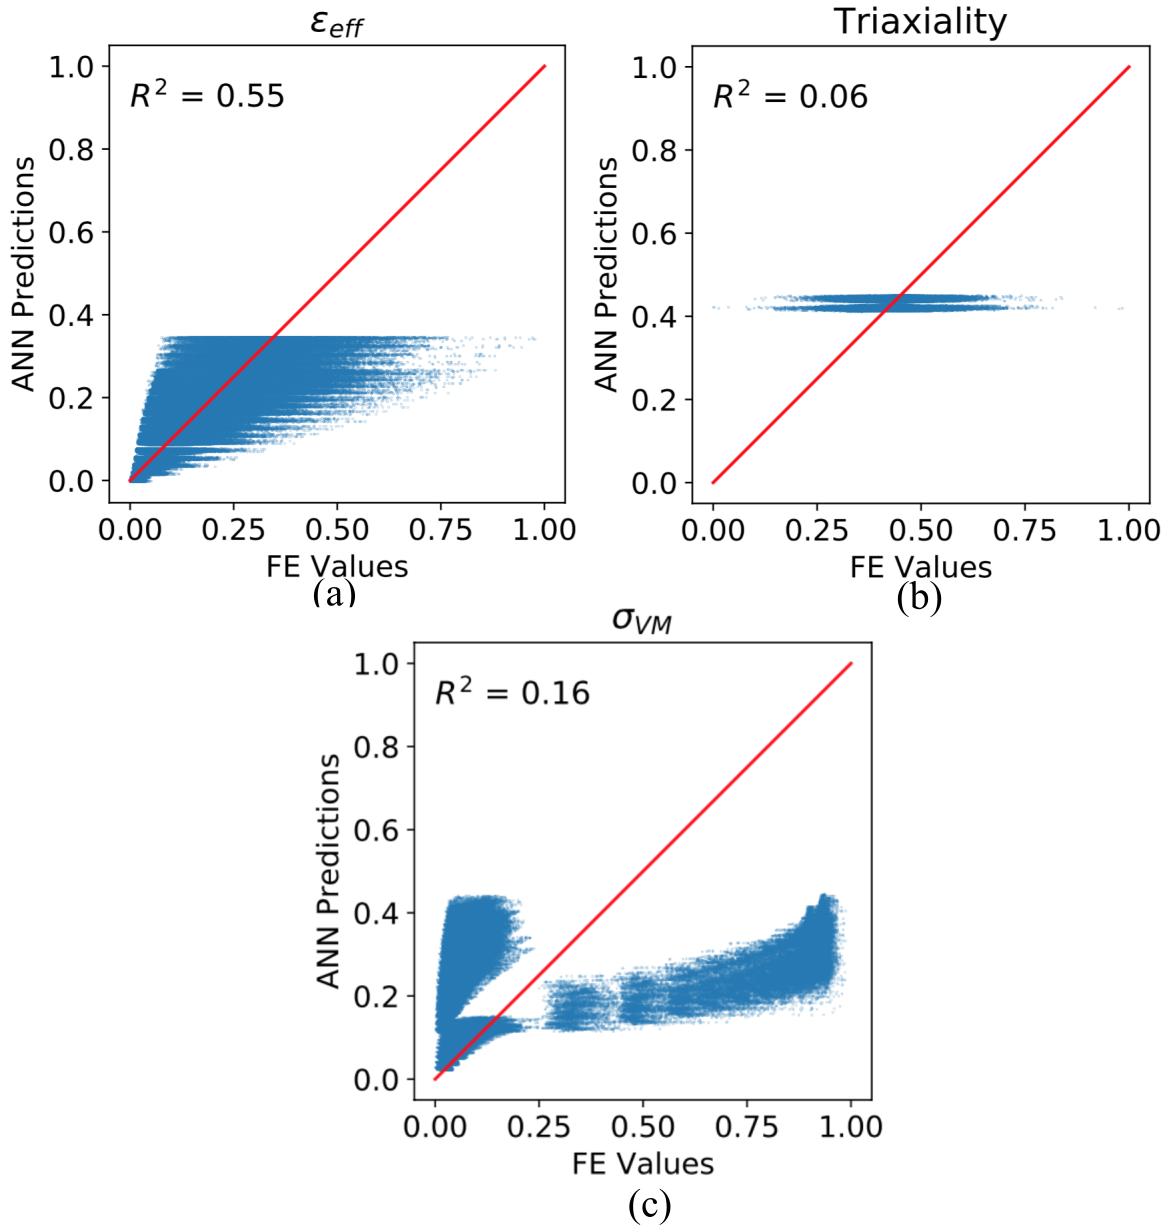
\includegraphics[width=0.9\textwidth]{Pictures/ann-res/final-ann-bitmap.png}
	\hspace{1mm}
	\caption{Plot of ANN predicted values vs FE values for (a) effective strain, (b) stress triaxiality ratio, and (c) von Mises effective stress. Note that all the variables are normalized.} 
	\label{fig:exp_pred_ann}
\end{figure}
A separate model was also trained to predict only one variable, effective strain. The architecture was kept the same, and the results showed an improvement in the $R^2$ value. We can conclude that predicting multiple variables using a single ANN leads to inaccuracy. Figure-\ref{fig:r2-ann} shows the $R^2$ values and figure-\ref{fig:ann-contours} shows the contour plots of ANN predicted value as compared to the true values. The numerical value of the predictions is quite inaccurate however, the ANN model has been able to locate some hotspots. 
\begin{figure}[!h]
	\centering
	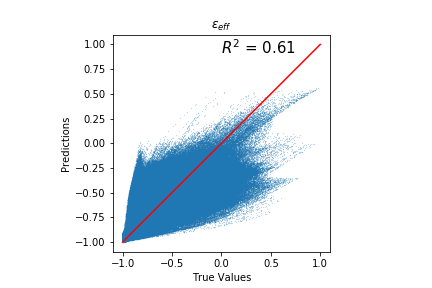
\includegraphics[width=0.9\textwidth]{Pictures/strain_eff_pred_exp.png}
	\hspace{1mm}
	\caption{Plot of ANN predicted values vs FE values for effective strain trained alone} 
	\label{fig:r2-ann}
\end{figure}

\begin{figure}[!h]
	\centering
	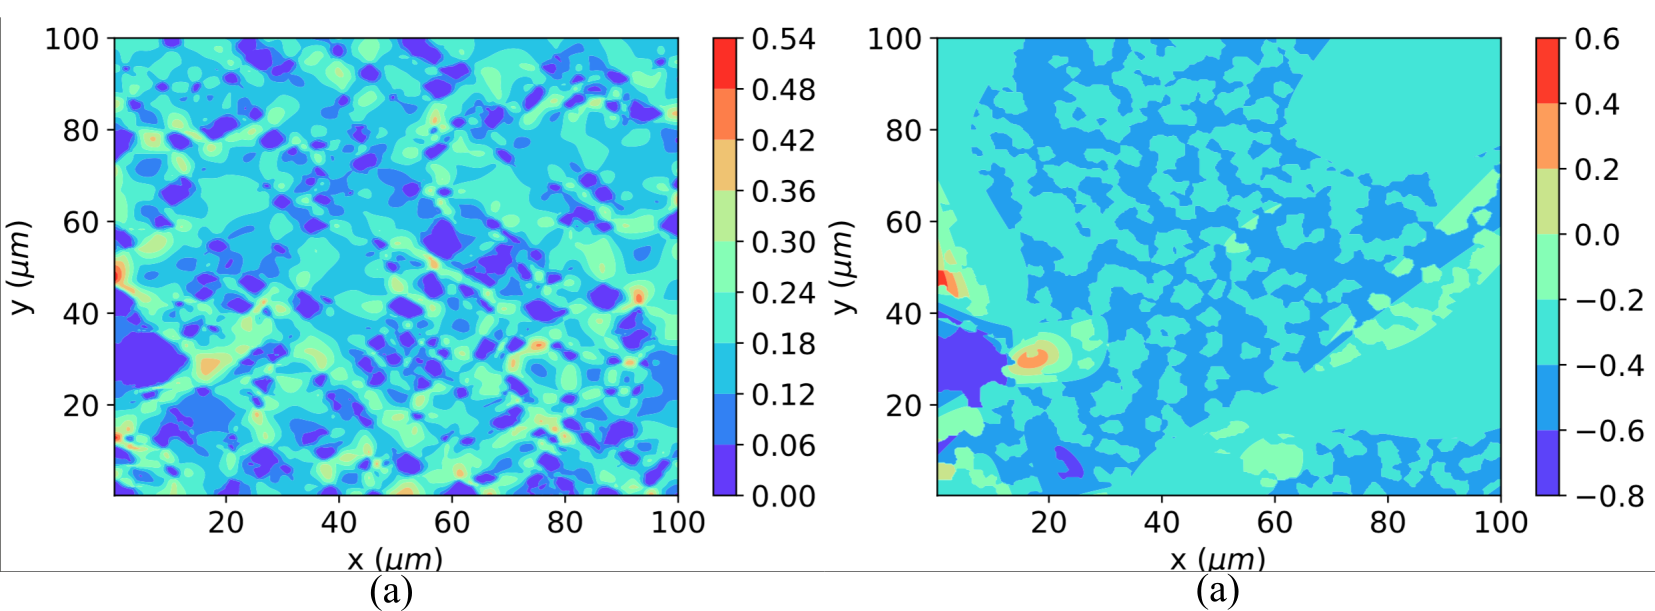
\includegraphics[width=0.95\textwidth]{Pictures/ann-res/ann-contours.png}
	\hspace{1mm}
	\caption{Effective Strain contour plots for (a) FE and (b) ANN predicted values.} 
	\label{fig:ann-contours}
\end{figure}
\newpage
\section{LSTM Model Results}
The LSTM Model shows significantly better performance than the ANN model. Plastic deformation being a history-dependent process, the output variable prediction is better modeled using LSTMs as they treat data as a time series. LSTMs maintain a context over time making them efficient in time series predictive modeling problems. Our model was able to achieve very high $R^2$ values for all the three output variables here, namely, effective strain (${\bar{\epsilon}}$), von Mises effective stress ($\bar{\sigma}$) and stress triaxiality ratio. The high accuracy of the model can be observed from the plots in
Figure \ref{fig:exp_pred_lstm}. Table \ref{tab:diff-lstm-table} shows results from LSTM models trained with different number of layers. Each layer contains 200 neurons and all the models take under 15 minutes to train. The training time here is 7 times less than our best ANN model. 

\begin{table}
\begin{center}
\begin{tabular}{|c|c|c|c|c|c|}
\hline
Layers & MSE & \multicolumn{3}{c|}{$R^2$} \\
\hline
 & & ${\bar{\epsilon}}$ & $\bar{\sigma}$ & tri \\
\hline
2 & $2.93 \times 10^{-6}$ & 0.89 & 0.99 & 0.51\\
4 & $2.78 \times 10^{-5}$ & 0.89 & 0.89 & 0.92\\
8 & $4.74 \times 10^{-5}$ & 0.90 & 0.96 & 0.97\\
16 & $0.02$ & -1.20 & 0.93 & 0.96\\
\hline
\end{tabular}
\end{center}
\caption{Study of accuracy of models with different depths. All layers have 200 neurons.}
\label{tab:diff-lstm-table}
\end{table}
\begin{figure}[!h]
	\centering
	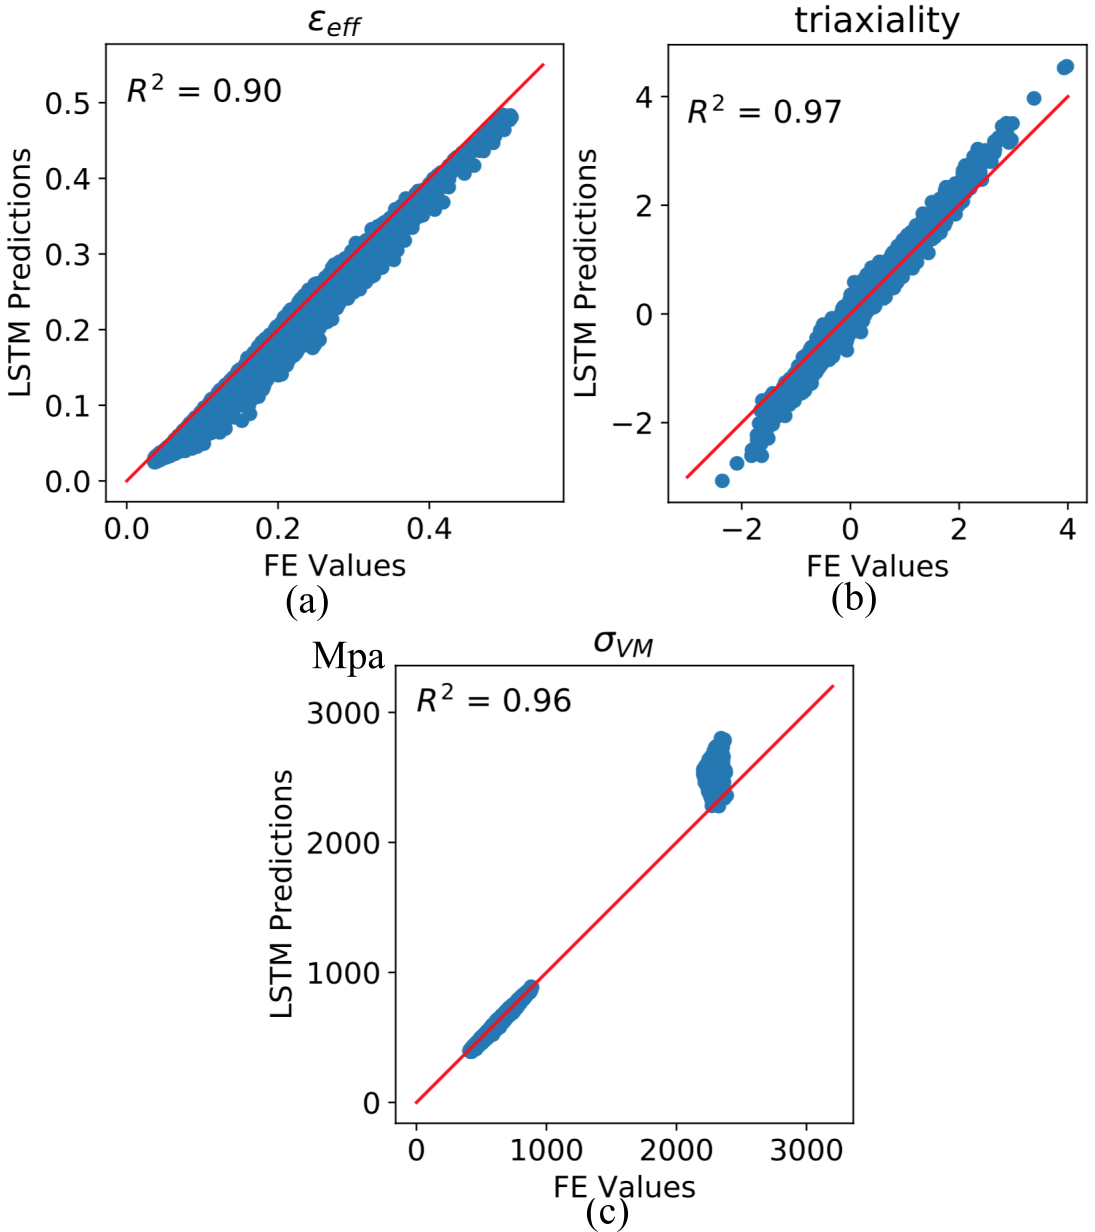
\includegraphics[width=0.8\textwidth]{Pictures/lstm-res/final-lstm-bitmap.png}
	\hspace{1mm}
	\caption{Plot of LSTM predicted values vs FE values for (a) effective strain, (b) triaxiality, (c) von Mises effective stress. Note that all the variables are normalized.} 
	\label{fig:exp_pred_lstm}
\end{figure}

Finally, figures \ref{fig:eff_strain_bitmap}, \ref{fig:tri_bitmap} and \ref{fig:vonmises_bitmap} show the contour plots for the different predicted variable at the last strain step. The contour plots depict how the model has successfully captured local behaviour of the microstructure. In figure-\ref{fig:vonmises_bitmap}, the predicted stress values higher than the FE values but the regions with high stress have been captured with good accuracy.
% \begin{figure}[hbtp]
% \begin{center}
% 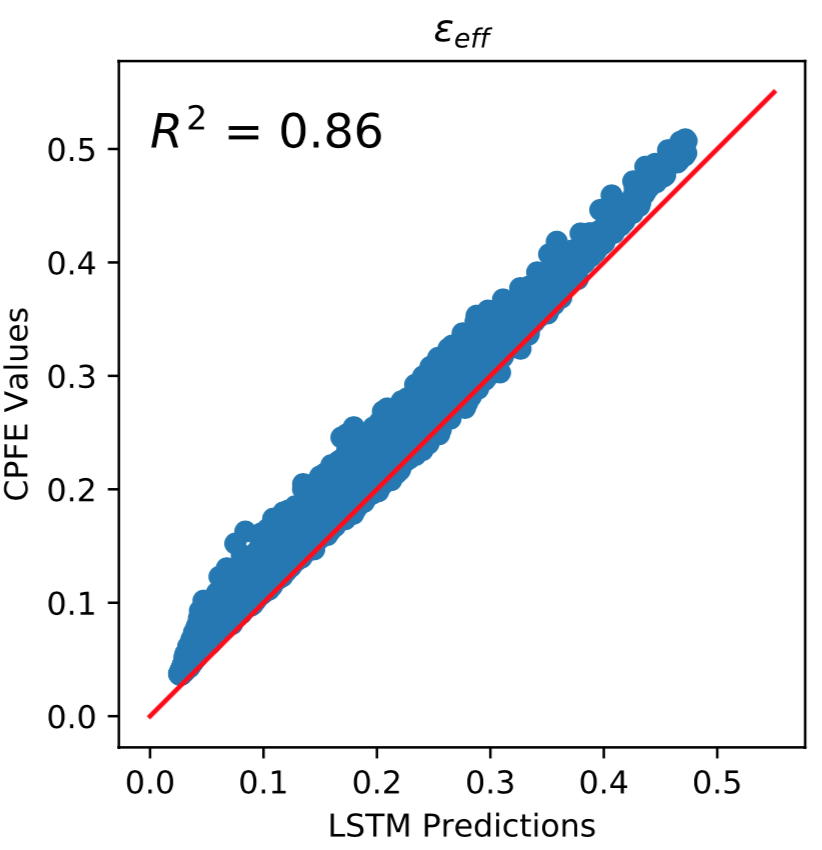
\includegraphics[scale=0.4]{Pictures/lstm-res/strain_eff.png}
% 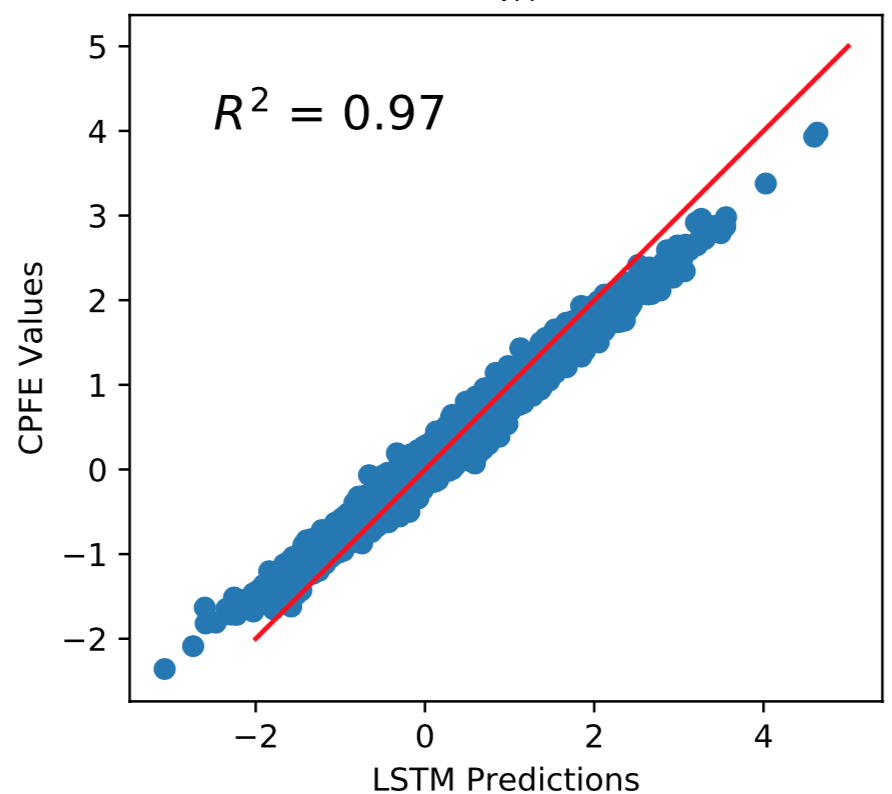
\includegraphics[scale=0.4]{Pictures/lstm-res/tri.png}
% \end{center}
% \begin{center}
% 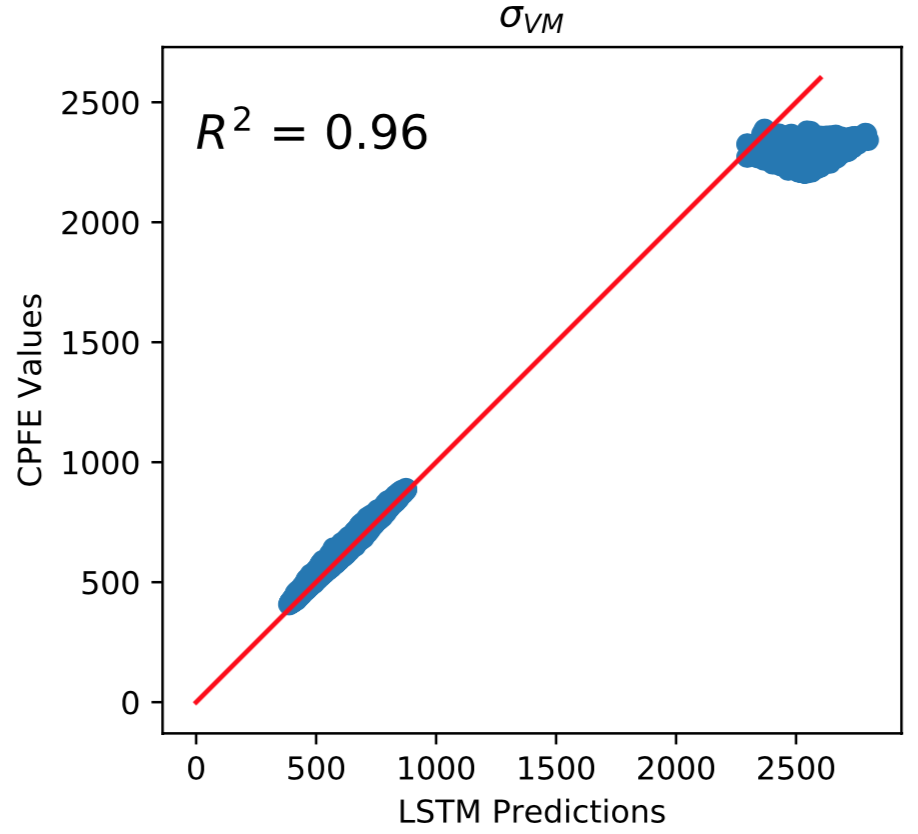
\includegraphics[scale=0.4]{Pictures/lstm-res/vonmises.png}
% \end{center}
% \caption{Plots of ANN Predictions vs CPFE Values for all the output variables}
% \label{fig:exp_pred_lstm}
% \end{figure}

\begin{figure}[!h]
	\centering
	\includegraphics[width=0.95\textwidth]{Pictures/lstm-res/eff_strain_bitmap.png}
	\hspace{1mm}
	\caption{Effective Strain contour plots for (a) FE and (b) LSTM predicted values.} 
	\label{fig:eff_strain_bitmap}
\end{figure}

\begin{figure}[!h]
	\centering
	\includegraphics[width=0.95\textwidth]{Pictures/lstm-res/tri_bitmap.png}
	\hspace{1mm}
	\caption{Triaxiality contour plots for (a) FE and (b) LSTM predicted values.} 
	\label{fig:tri_bitmap}
\end{figure}

\begin{figure}[!h]
    \centering
	\includegraphics[width=0.95\textwidth]{Pictures/lstm-res/vonmises_bitmap-units.png}
	\hspace{1mm}
	\caption{Vonmises contour plots for (a) FE and (b) LSTM predicted values.} 
	\label{fig:vonmises_bitmap}
\end{figure} 
%% Chapter Template

\chapter{Conclusion} % Main chapter title

\label{Chapter5} % Change X to a consecutive number; for referencing this chapter elsewhere, use \ref{ChapterX}

\lhead{Chapter 5. \emph{Conclusion}} % Change X to a consecutive number; this is for the header on each page - perhaps a shortened title

%----------------------------------------------------------------------------------------
%	SECTION 1
%----------------------------------------------------------------------------------------

\section{Summary}

We have applied two machine learning models, namely, artificial neural networks (ANNs) and long short term memory (LSTM), a type of recurrent neural network (RNN) to predict the deformation of DP steel microstructures. J2 plasticity simulations are run for the 2D dual-phase ferrite-martensite microstructures. The results of these simulations are used as the ground truth for the machine learning model training. We start with employing an ANN to make predictions for effective strain, von Mises effective stress and triaxiality. After a systematic parametric study for the hyper parameters of the model, the accuracy of the ANN models was found to be very low. ANNs do not deal with temporal or spatial information. The higher errors may also be a result of discretizing our dataset into $0.01$ strain steps. 

As plasticity is a history-dependent process, RNNs are presumably a better option. LSTMs were applied to deal with the temporal nature of our data. The results obtained from LSTM model have an error value 3 order less than that of the ANN. The model makes predictions at $0.01$ strain intervals. Our method does not need to perform numerical iterations per strain step, otherwise needed by the conventional methods. The main strength of the LSTM model over ANN, is the reduction in computational time. The training time is 7 to 8 times less than that for ANN and predictions only take a few seconds. This ML-surrogate model trained and tested on simulated data is highly accurate and orders of magnitude faster than conventional micromechanical models. 

\section{Future Work}
The models developed has been trained and tested for microstructure with defined phase fractions and fixed boundary conditions. The framework can be extended to predict the evolution of series of other mircomechanical properties. Furthermore, more microstructures can be generated with various macroscopic conditions and microstructure evolution for a more general case can be predicted.  
%\input{Chapters/Chapter6} 
%\input{Chapters/Chapter7} 

%----------------------------------------------------------------------------------------
%	THESIS CONTENT - APPENDICES
%----------------------------------------------------------------------------------------

\addtocontents{toc}{\vspace{2em}} % Add a gap in the Contents, for aesthetics

\appendix % Cue to tell LaTeX that the following 'chapters' are Appendices

% Include the appendices of the thesis as separate files from the Appendices folder
% Uncomment the lines as you write the Appendices

% % Appendix Template

\chapter{Appendix A} % Main appendix title

\label{AppendixX} % Change X to a consecutive letter; for referencing this appendix elsewhere, use \ref{AppendixX}

\lhead{Appendix X. \emph{Appendix Title Here}} % Change X to a consecutive letter; this is for the header on each page - perhaps a shortened title

Write your Appendix content here.

% %\input{Appendices/AppendixB}
% %\input{Appendices/AppendixC}

% \addtocontents{toc}{\vspace{2em}} % Add a gap in the Contents, for aesthetics

% \backmatter

%----------------------------------------------------------------------------------------
%	BIBLIOGRAPHY
%----------------------------------------------------------------------------------------
\nocite{*}
\label{Bibliography}

\lhead{\emph{Bibliography}} % Change the page header to say "Bibliography"

\bibliographystyle{ieeetr} % Use the "custom" BibTeX style for formatting the Bibliography

\bibliography{Bibliography} % The references (bibliography) information are stored in the file named "Bibliography.bib"

\end{document}  
